%%%%%%%%%%%%%%%%%%%%%%%%%%%%%%%%%%%%%%%%%%%%%%%%%%%%%%%%%%%%%%%%%%%%%%%%%%%%%%%%
%% Plantilla de memoria en LaTeX para la EIF - Universidad Rey Juan Carlos
%%
%% Por Gregorio Robles <grex arroba gsyc.urjc.es>
%%     Grupo de Sistemas y Comunicaciones
%%     Escuela de Ingeniería de Fuenlabrada
%%     Universidad Rey Juan Carlos
%% (muchas ideas tomadas de Internet, colegas del GSyC, antiguos alumnos...
%%  etc. Muchas gracias a todos)
%%
%% La última versión de esta plantilla está siempre disponible en:
%%     https://github.com/gregoriorobles/plantilla-memoria
%%
%% Para obtener PDF, ejecuta en la shell:
%%   make
%% (las imágenes deben ir en PNG o JPG)

%%%%%%%%%%%%%%%%%%%%%%%%%%%%%%%%%%%%%%%%%%%%%%%%%%%%%%%%%%%%%%%%%%%%%%%%%%%%%%%%

\documentclass[a4paper, 12pt]{book}
%\usepackage[T1]{fontenc}

\usepackage{textcomp}
\usepackage[hidelinks]{hyperref}
\usepackage{xcolor}
\usepackage[a4paper, left=2.5cm, right=2.5cm, top=3cm, bottom=3cm]{geometry}
\usepackage{times}
\usepackage[utf8]{inputenc}
\usepackage[spanish]{babel} % Comenta esta línea si tu memoria es en inglés
\usepackage{url}
\usepackage{listings}
%\usepackage[dvipdfm]{graphicx}
\usepackage{graphicx}
\usepackage{caption}
\usepackage{float}  %% H para posicionar figuras
\usepackage[nottoc, notlot, notlof, notindex]{tocbibind} %% Opciones de índice
\usepackage{latexsym}  %% Logo LaTeX
\usepackage{pgfgantt}
\usepackage{pdflscape}

\definecolor{codegray}{RGB}{100,100,100} % Puedes ajustar el gris aquí

\lstset{
  basicstyle=\ttfamily\scriptsize\color{codegray},
  showstringspaces=false,
  breaklines=true,
  numbers=none,
  language={},        
  keywordstyle=,
  commentstyle=,
  stringstyle=,
  identifierstyle=,
}

% Escribe el título y el nombre del autor / autora para que se use bien
% en otras partes de la plantilla
% Dependiendo de las partes de la plantilla, a veces aparecerán tal
% cual los escribas, a veces totalmente en mayúsculas, a veces de otras
% formas
\title{SISTEMA DE SEGUIMIENTO DE MANOS PARA ESCENAS EN REALIDAD EXTENDIDA (XR)}
\author{Juan José Arias Rojas}

% Guarda el título, el autor y la fecha en variables
\makeatletter
\let\thetitle\@title
\let\theauthor\@author
\let\thedate\@date
\makeatother

\renewcommand{\baselinestretch}{1.5}  %% Interlineado

\begin{document}

\renewcommand{\refname}{Bibliografía}  %% Renombrando
\renewcommand{\appendixname}{Apéndice}


%%%%%%%%%%%%%%%%%%%%%%%%%%%%%%%%%%%%%%%%%%%%%%%%%%%%%%%%%%%%%%%%%%%%%%%%%%%%%%%%
% PORTADA

\begin{titlepage}
	\begin{center}
		\includegraphics[scale=0.6]{img/URJ_logo_Color_POS.png}

		\vspace{1.75cm}

		\LARGE
		ESCUELA DE INGENIERÍA DE FUENLABRADA
		\vspace{1cm}

		\LARGE
		GRADO EN INGENÍERIA EN SISTEMAS AUDIOVISUALES Y MULTIMEDIA

		\vspace{1cm}
		\LARGE
		\textbf{TRABAJO FIN DE GRADO}

		\vspace{2cm}

		\Large
		\MakeUppercase{\thetitle}

		\vspace{2cm}

		\large
		Autor : \theauthor \\
		Tutor : Dr. Jesús María González Barahona\\
		\vspace{1cm}

		\large
		Curso académico 2024/2025

	\end{center}
\end{titlepage}

\newpage
\mbox{}
\thispagestyle{empty} % para que no se numere esta pagina



%%%%%%%%%%%%%%%%%%%%%%%%%%%%%%%%%%%%%%%%%%%%%%%%%%%%%%%%%%%%%%%%%%%%%%%%%%%%%%%%
%%%% Licencia
\clearpage
\pagenumbering{gobble}
\chapter*{}

\vspace{12cm}


\begin{flushright}
	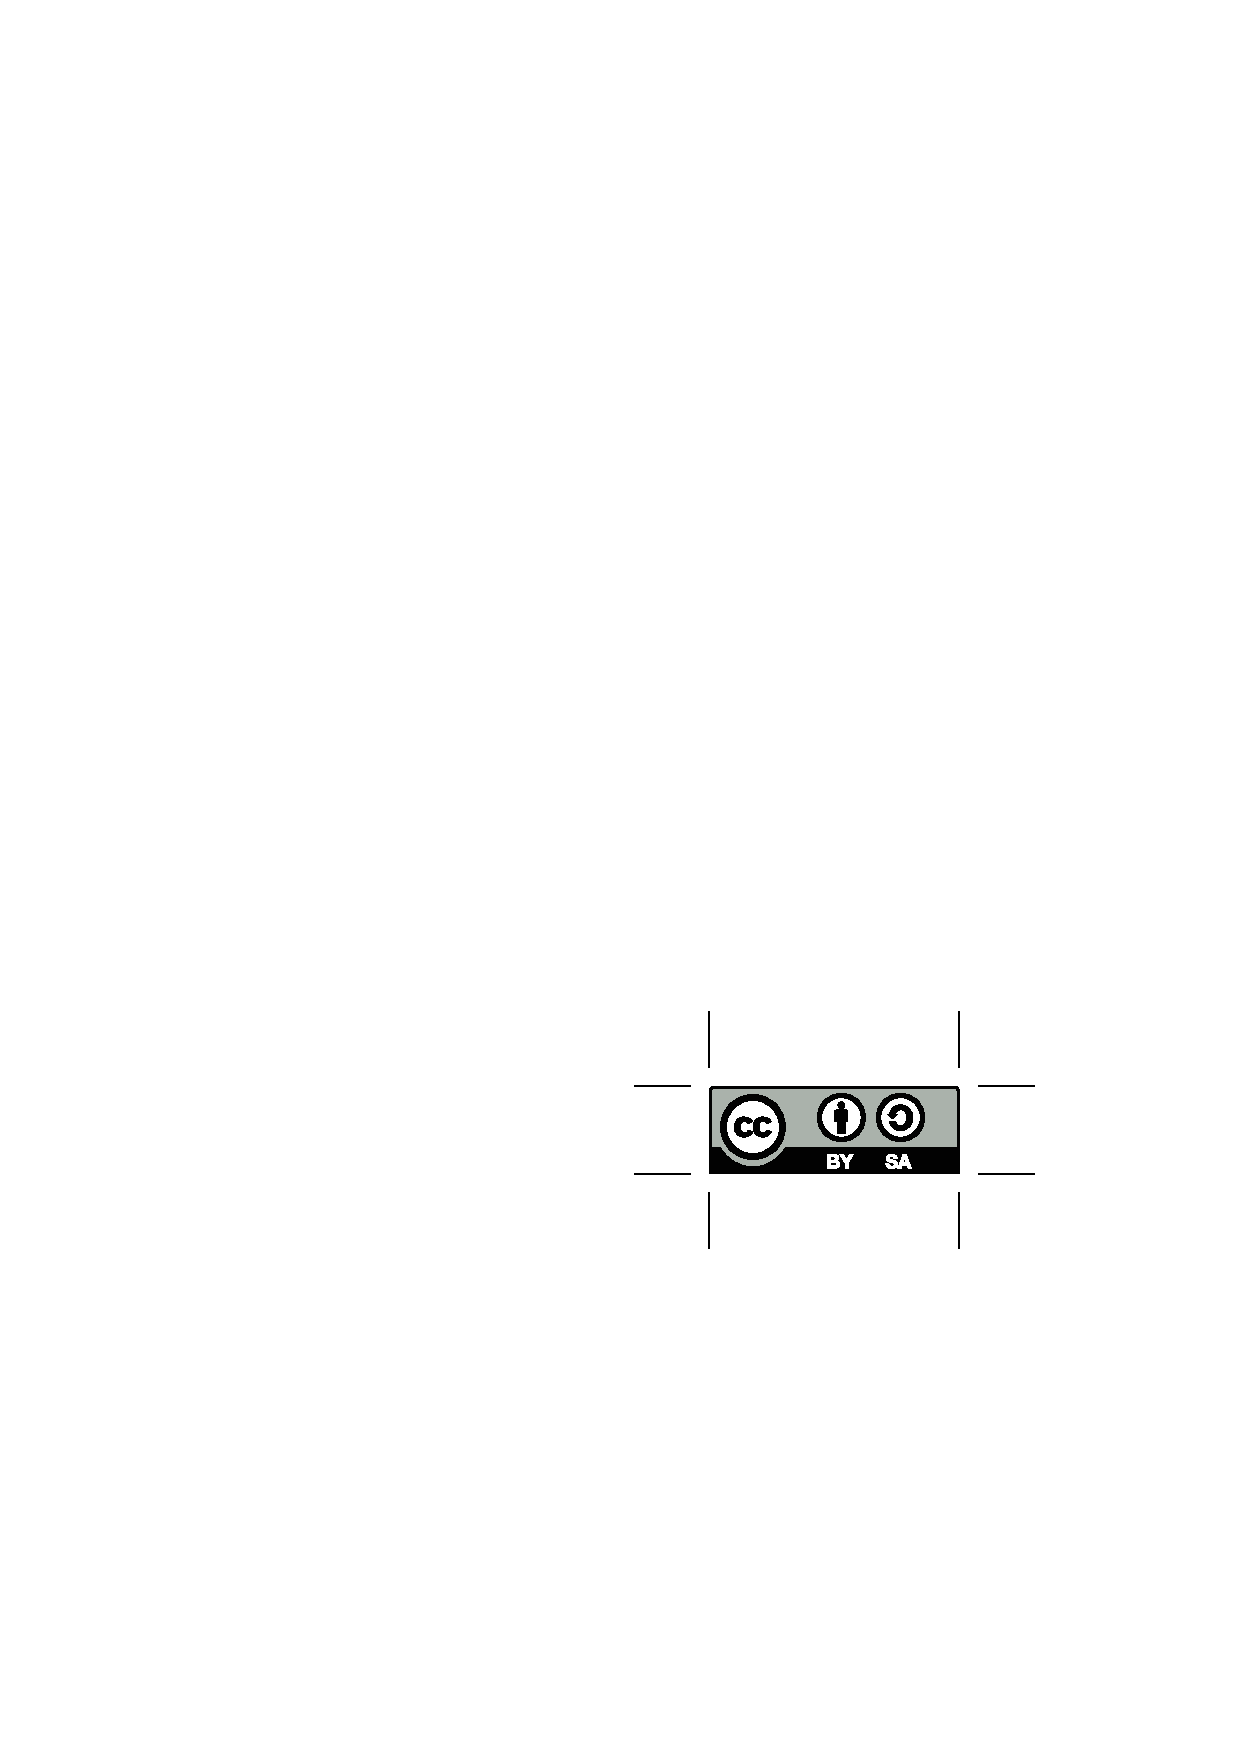
\includegraphics[scale=0.6]{img/by-sa}
	%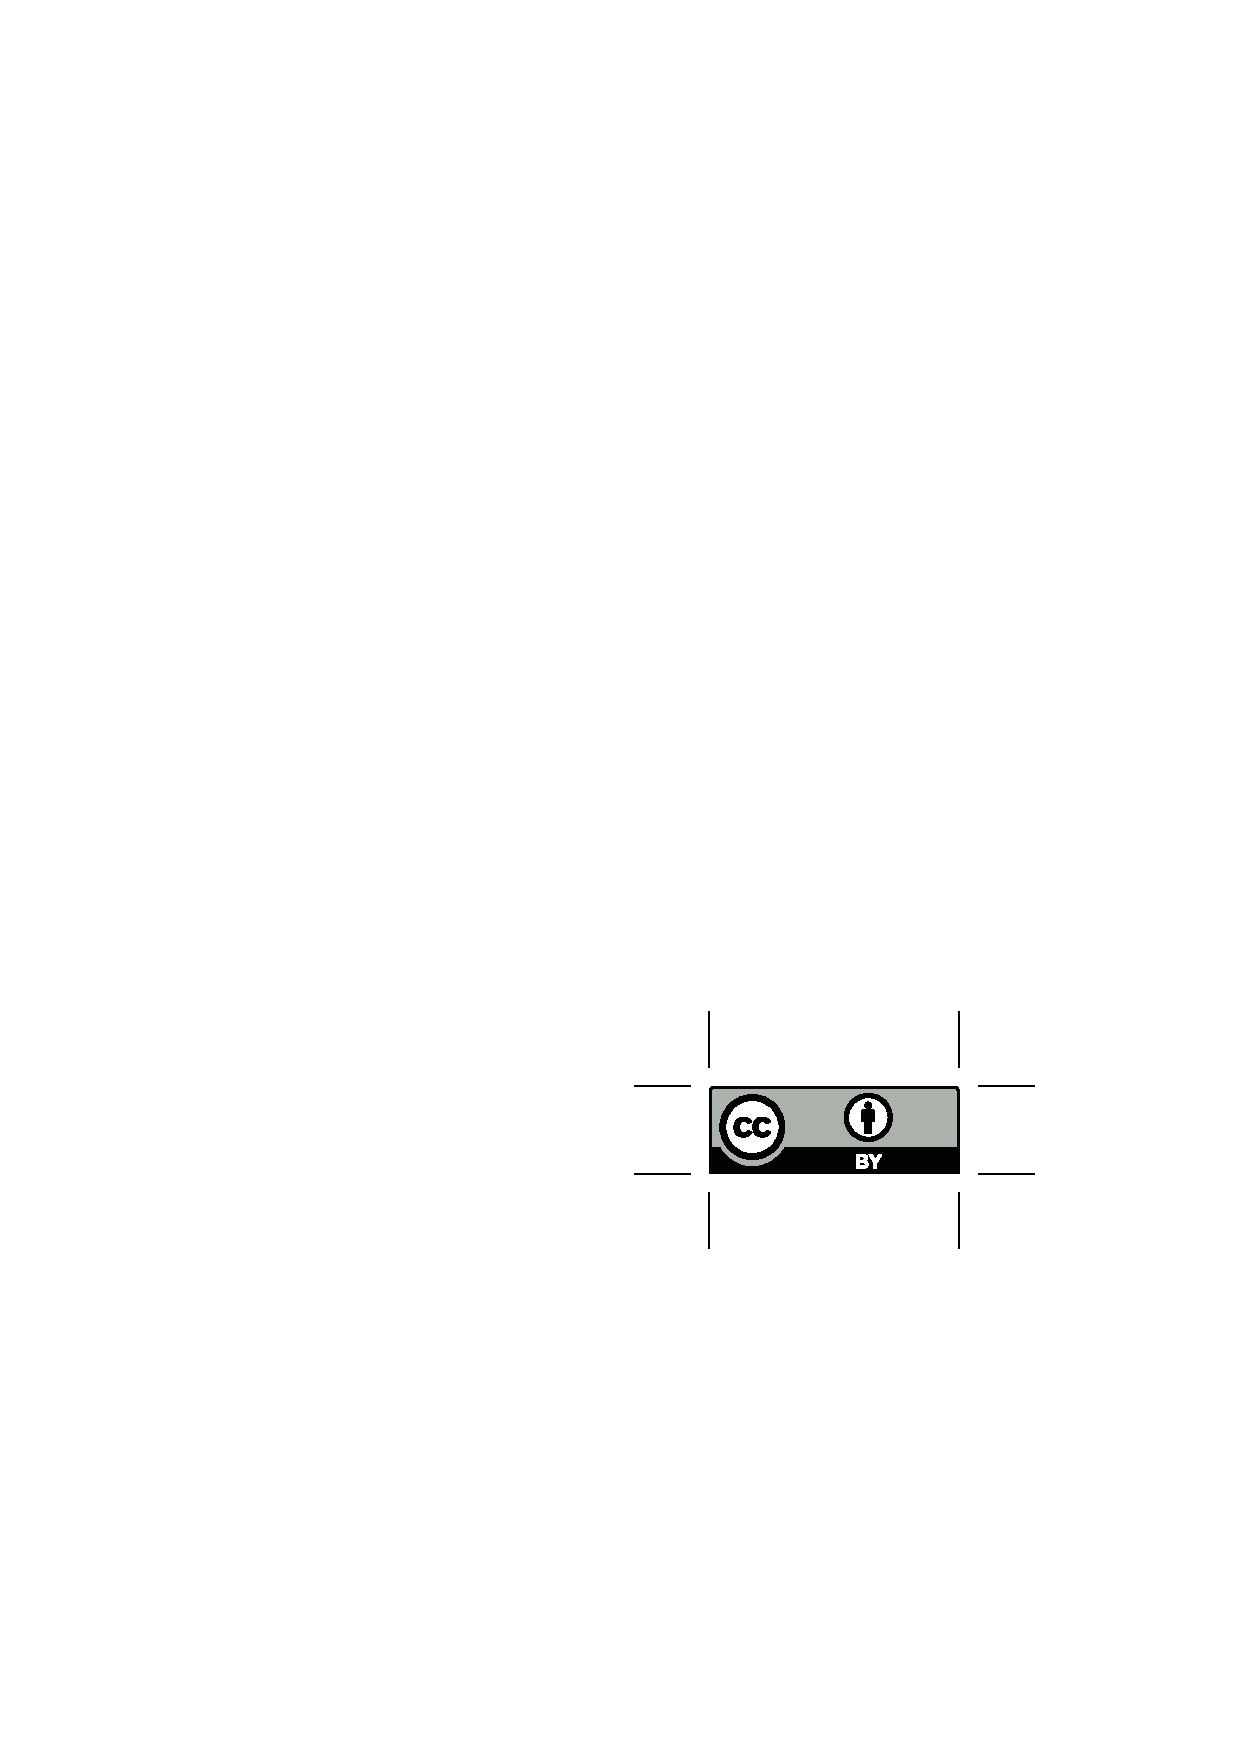
\includegraphics[scale=0.6]{img/by}

	%% Poner el año adecuado
	\noindent©2025 \theauthor  \\
	Algunos derechos reservados  \\
	Este documento se distribuye bajo la licencia \\
	``Atribución-CompartirIgual 4.0 Internacional'' de Creative Commons, \\
	disponible en \\
	\url{https://creativecommons.org/licenses/by-sa/4.0/deed.es}
\end{flushright}

%%%%%%%%%%%%%%%%%%%%%%%%%%%%%%%%%%%%%%%%%%%%%%%%%%%%%%%%%%%%%%%%%%%%%%%%%%%%%%%%
%%%% Dedicatoria

\chapter*{}
\pagenumbering{Roman} % para comenzar la numeracion de paginas en numeros romanos
\begin{flushright}
	\textit{Dedicado a \\
		todos aquellos que me animaron y apoyaron \\
		incluso en mis momentos de debilidad}
\end{flushright}

%%%%%%%%%%%%%%%%%%%%%%%%%%%%%%%%%%%%%%%%%%%%%%%%%%%%%%%%%%%%%%%%%%%%%%%%%%%%%%%%
%%%% Agradecimientos

\chapter*{Agradecimientos}
%\addcontentsline{toc}{chapter}{Agradecimientos} % si queremos que aparezca en el índice
\markboth{AGRADECIMIENTOS}{AGRADECIMIENTOS} % encabezado 
Ha sido un camino de 5 años, pero al fin llega a su fin. Quiero agradecerle a mi familia por estar siempre a mi lado, apoyándome cuando lo necesitaba, por los sacrificios que han hecho con el fin de que yo llegue hasta aquí, por conseguirme el coche que me permitía ir todos los días a la universidad y ayudarme con la gasolina. 

También quiero agradecerle a mi pareja, que pese a que nuestros caminos se cruzaron a mitad de este viaje, desde el momento en el que te conocí, tú siempre has estado a mi lado, siempre me has apoyado y siempre me has animado. Tú más que nadie me has dado la fuerza necesaria para poder seguir adelante hasta cumplir mi meta y espero poder ayudarte tanto como tú me has ayudado a mí. 

%%%%%%%%%%%%%%%%%%%%%%%%%%%%%%%%%%%%%%%%%%%%%%%%%%%%%%%%%%%%%%%%%%%%%%%%%%%%%%%%
%%%% Resumen

\chapter*{Resumen}
%\addcontentsline{toc}{chapter}{Resumen} % si queremos que aparezca en el índice
\markboth{RESUMEN}{RESUMEN} % encabezado
El seguimiento de manos es una tecnología de Realidad Extendida (XR) que cada vez se usa más, pero hoy en día todavía afronta muchos obstáculos, ya sea porque no está muy desarrollada o tiene un uso muy limitado. Estos obstáculos hacen que los usuarios tiendan a usar más los controladores de los dispositivos VR, lo cual dificulta en cierta medida la sensación de inmersión dentro de escenas virtuales. 

Este Trabajo de Fin de Grado se centra en dar un paso más en la evolucionando del sistema de seguimiento de manos para entornos virtuales, consiste en el desarrollo de un sistema de detección y renderización de manos que permita a los usuarios 
poder interactuar con los distintos elementos de la escena de forma natural y fluida.

El proyecto se ha creado utilizado A-Frame, un framework el cual permite la creación y configuración de escenas tanto AR como VR dentro de un navegador compatible con WebGL, al utilizar el navegador para el seguimiento de manos se utilizó WebXR, un framework diseñado para crear experiencias inmersivas en el navegador mediante la realidad extendida. El sistema resultante permite a los usuarios visualizar sus manos dentro del entorno virtual, mientras que son capaces de realizar distintas acciones con estas, permitiendo así una mayor inmersión en la escena.

%%%%%%%%%%%%%%%%%%%%%%%%%%%%%%%%%%%%%%%%%%%%%%%%%%%%%%%%%%%%%%%%%%%%%%%%%%%%%%%%
%%%% Resumen en inglés

\chapter*{Summary}
%\addcontentsline{toc}{chapter}{Summary} % si queremos que aparezca en el índice
\markboth{SUMMARY}{SUMMARY} % encabezado
Hand detection is an increasingly utilized Extended Reality (XR) technology, yet it still faces many obstacles today, either due to its underdeveloped state or its limited application. These challenges often lead users to favor VR device controllers, which somewhat hinders the sense of immersion within virtual scenes.

This Bachelor's Thesis focuses on advancing the evolution of hand detection systems for virtual environments. It involves the development of a hand detection and rendering system that allows users to naturally and fluidly interact with various elements within a scene.

The project was created using A-Frame, a framework that allows for the creation and configuration of both AR and VR scenes within a WebGL-compatible browser. For hand tracking within the browser, WebXR was utilized, a framework designed for creating immersive experiences in the browser through extended reality. The resulting system allows users to visualize their hands within the virtual environment while being able to perform various actions with them, thereby enabling greater immersion in the scene.
%%%%%%%%%%%%%%%%%%%%%%%%%%%%%%%%%%%%%%%%%%%%%%%%%%%%%%%%%%%%%%%%%%%%%%%%%%%%%%%%
%%%%%%%%%%%%%%%%%%%%%%%%%%%%%%%%%%%%%%%%%%%%%%%%%%%%%%%%%%%%%%%%%%%%%%%%%%%%%%%%
% ÍNDICES %
%%%%%%%%%%%%%%%%%%%%%%%%%%%%%%%%%%%%%%%%%%%%%%%%%%%%%%%%%%%%%%%%%%%%%%%%%%%%%%%%

% Las buenas noticias es que los índices se generan automáticamente.
% Lo único que tienes que hacer es elegir cuáles quieren que se generen,
% y comentar/descomentar esa instrucción de LaTeX.

%%%% Índice de contenidos
\tableofcontents
%%%% Índice de figuras
\cleardoublepage
%\addcontentsline{toc}{chapter}{Lista de figuras} % para que aparezca en el indice de contenidos
\listoffigures % indice de figuras
%%%% Índice de tablas
%\cleardoublepage
%\addcontentsline{toc}{chapter}{Lista de tablas} % para que aparezca en el indice de contenidos
%\listoftables % indice de tablas


%%%%%%%%%%%%%%%%%%%%%%%%%%%%%%%%%%%%%%%%%%%%%%%%%%%%%%%%%%%%%%%%%%%%%%%%%%%%%%%%
%%%%%%%%%%%%%%%%%%%%%%%%%%%%%%%%%%%%%%%%%%%%%%%%%%%%%%%%%%%%%%%%%%%%%%%%%%%%%%%%
% INTRODUCCIÓN cpitulo 1%
%%%%%%%%%%%%%%%%%%%%%%%%%%%%%%%%%%%%%%%%%%%%%%%%%%%%%%%%%%%%%%%%%%%%%%%%%%%%%%%%

\cleardoublepage
\chapter{Introducción}
\label{sec:intro} % etiqueta para poder referenciar luego en el texto con ~\ref{sec:intro}
\pagenumbering{arabic} % para empezar la numeración de página con números
La realidad virtual es un campo que cada vez toma mayor peso, e introducir al usuario cada vez más dentro del entorno virtual ha sido uno de los principales objetivos desde el comienzo. Al principio y hoy en día, la principal 
solución para mejorar las interfaces de usuario en Realidad Extendida (XR), era el uso de los controladores de los distintos dispositivos VR. Pero el uso de los controladores no era natural en comparación al empleo de las manos, así que se inició el desarrollo del seguimiento de manos. Hoy en 
día, el seguimiento de manos está muy extendido, sin embargo, la utilización de los controladores sigue predominando, puesto que las tecnologías de seguimiento de manos no están tan desarrolladas. El empleo de estos controladores supone una limitación, produciendo una sensación de inmersión en la escena virtual no tan profunda como se podría desear, ya que 
el control de las distintas entidades que pueda haber no resulta tan natural para el usuario.  

Aunque al principio con los dispositivos VR únicamente se podían ver videos sin posibilidad de interactuar con ellos, la necesidad de ser capaces de interactuar con esas escenas con el tiempo se volvió una necesidad, sobre todo cuando se empezaron a desarrollar las primeras aplicaciones o servicios para los dispositivos. 
Esta necesidad ha tenido bastantes formas de cubrirla, la principal y más usada incluso hoy en día, es el uso de controladores, aunque también se han llegado a desarrollar trajes o guantes especiales que permiten al usuario tener una mayor sensación de inmersión, aunque estas últimas opciones eran muy caras y poco asequibles para la mayoría de personas. Por eso,
el desarrollo de sistemas capaces de detectar y seguir las manos tomaron importancia.

Como se menciono antes, el seguimiento de manos es una tecnología que surgió a raíz de la necesidad de poder interactuar con la escena de forma más natural y fluida, cosa que no se conseguía con el uso de controladores. Al principio, para lograr esto se hacía uso de unos guantes especiales, los cuales tenían una serie de sensores que detectaba el dispositivo VR y representaba en la escena, siendo así una tecnología similar a la que se usa en la industria del cine.
Pero estos guantes eran demasiado caros y poco accesibles para la mayoría de personas, hoy en día aún existen modelos de estos guantes, pero siguen teniendo el mismo problema de precio y accesibilidad. Para solucionar esto, se empezó el desarrollo de sistemas de detección y seguimiento de manos que no requerían el uso de hardware adicional, únicamente con el empleo de las gafas VR era suficiente. 

Este proyecto se centra en dar un paso más en la evolución del seguimiento de manos, permitiendo que los usuarios puedan utilizar sus manos dentro de los distintos entornos virtuales que estos creen en sus navegadores a través de A-Frame. 
Esto permite a los usuarios interactuar con los elementos de la escena de una forma más natural. Hoy en día ya existen componentes nativos en A-Frame que permiten el seguimiento de manos, pero su funcionamiento es muy limitado, permitiendo únicamente agarrar elementos de la escena.
Mi proyecto va un paso más allá de eso, permitiendo la detección de varios gestos de la mano y la ejecución de diferentes acciones al realizar dichos gestos, lo cual contrasta bastante con la tecnología actual, en la cual únicamente están implementados un gesto y una acción.
Además de las acciones y gestos implementados en este proyecto, la forma de su diseño la convierte en una tecnología escalable y adaptable para la creación de distintas escenas o aplicaciones VR. 

Siguiendo el siguiente \textit{enlace}\footnote{\url{https://jujoarias.github.io/TFG/}} se accede a la página web creada para este proyecto, donde se encuentra un enlace al repositorio GitHub, un enlace a la presentación, otro a esta memoria y a una segunda página donde se encuentran todas las demos que se mencionan en este proyecto, además de unos videos que muestran algunas de las escenas creadas.

\section{Contexto}
\label{sec:contexto}
La realidad virtual (VR) tiene sus orígenes en 1963, cuando el escritor Hugo Gernsback, presento su prototipo de gafas inmersivas \texttt{The Teleyeglasses}. La idea de este prototipo era la de permitir a los usuarios sentirse como si estuvieran dentro del mundo de la televisión, al sujetar una televisión en miniatura a la cabeza como si fuesen unas gafas. Años más tarde, en 1968, el científico de la computación Ivan Sutherland del MIT,
desarrolló \texttt{The Sword of Damocles}, dicho sistema hoy en día se considera como el padre de las gafas de realidad virtual modernas. Este sistema incluía un casco sostenido por un brazo mecánico desde el techo, y utilizaba pantallas CRT para proyectar gráficos básicos que respondían al movimiento de la cabeza del usuario.
Estos dispositivos sentaron las bases para la evolución de la realidad virtual. 

Más tarde, cuando Palmer Luckey inicio su campaña para la creación de las Oculus Rift, llamo la atención de Facebook, la cual compro la empresa de Palmer en 2014. Desde entonces, la industria de la realidad virtual ha ido creciendo a pasos agigantados con la llegada de diversos dispositivos. Gracias a su versatilidad, la realidad virtual ha conseguido implantarse en áreas como el entretenimiento, la medicina o la educación. Hoy en día grandes empresas como Apple o Meta 
realizan grandes inversiones para seguir desarrollando estas tecnologías con el objetivo de potenciar la realidad virtual y hacerla más accesible.  

Gracias a que grandes empresas invierten muchos recursos, la realidad virtual ha avanzado mucho, pero aún le queda mucho por mejorar. Desde hace años, las tecnologías de Realidad Extendida (XR) han sido uno de los principales pilares de la realidad virtual, en especial el seguimiento de manos. Aunque el seguimiento de manos es una tecnología que se usa desde hace años, no está tan desarrollada como otros campos. Esto se debe a que en la mayoría de ocasiones es necesario 
utilizar los controladores de los distintos dispositivos VR, puesto que el uso del handtracking está muy limitado o es poco fluido. 
Mi trabajo de fin de grado se centra en el desarrollo de una tecnología de seguimiento de manos que permita a los usuarios interactuar, de forma más natural y fluida, con distintos elementos de la escena mediante escenas que estén dentro de un navegador. 

\section{Objetivos}
\label{sec:objetivos}

\subsection{Objetivo general}
\label{subsec:objetivo-general}
Este consiste en el desarrollo de un sistema de seguimiento de manos que permita la interacción fluida y natural con elementos de la escena y que funcione dentro de un navegador, mediante gestos que realice el usuario. Este sistema se plantea como una caja de herramientas que posteriormente 
pueden ser utilizadas para la creación de distintas escenas/aplicaciones inmersivas para el navegador.
\subsection{Objetivos específicos}
\label{subsec:objetivos-especificos}
A continuación se describen los diversos objetivos secundarios que fueron necesarios para realizar el objetivo principal.
\begin{itemize}
  \item \textbf{Estudio de opciones actuales de seguimiento de manos en A-Frame:} Estudio de los distintos componentes ya existentes de A-Frame dedicados al seguimiento de manos.
  \item \textbf{Estudio del seguimiento de manos:} Estudio e implementación de WebXR dentro de A-Frame para obtener los datos necesarios de las manos para posteriormente su renderización.
  \item \textbf{Implementar una herramienta de renderización de manos en A-Frame:} Construir un componente capaz renderizar las manos dentro del entorno virtual de la escena que reaccione de forma fluida a los movimientos del usuario, mientras mantiene una estructura realista que asemeje las manos reales. 
  \item \textbf{Implementar detección de gestos:} Desarrollar un sistema capaz de detectar y distinguir los distintos gestos que puede realizar el usuario con sus manos.
  \item \textbf{Implementación de acciones:} Creación de una serie de componentes capaces de reaccionar a los distintos gestos del usuario para que estos realicen distintas acciones dependiendo del gesto y la intención del usuario. 
  \item \textbf{Compatibilidad con el dispositivo Quest3:} Asegurar que el sistema resultante sea compatible con las Quest3.
  \item \textbf{Integración con otros componentes nativos de A-Frame:} Implementar el sistema de forma que sea posibilidad de poder integrar otros componentes nativos de A-Frame a la escena y que sean compatibles.
\end{itemize}

\section{Estructura de la memoria}
\label{subsec:estructura}
En esta sección se presenta la estructura de esta memoria, organizada en capítulos:

\begin{itemize}
  \item \hyperref[chap:tecnologias]{\textbf{Tecnologías utilizadas:}} Este capítulo enumera y describe las distintas tecnologías que han sido utilizadas a lo largo de todo el proyecto. Dichas tecnologías están divididas en principales y auxiliares y en cada una, además de su funcionalidad, se describe su importancia en el desarrollo del proyecto.
  \item \hyperref[chap:resultados]{\textbf{Descripción de los resultados obtenidos:}} Aquí se presenta el resultado final del proyecto. Se describe de forma detallada la arquitectura de los distintos componentes que se han creado, al igual que se da una explicación de cara al usuario para que sea capaz de manejarse dentro de la escena y pueda interactuar con los elementos en ella. 
  \item \hyperref[chap:Desarrollo del proyecto]{\textbf{Desarrollo del proyecto:}} Este capítulo describe el proceso que ha sido necesario para llegar a los resultados obtenidos. Se describe siguiendo la metodología \texttt{Agile}, dividiendo el proceso en distintos sprints donde cada uno tiene sus propios objetivos y resultados.
  \item \hyperref[chap:pruebas-experimentos]{\textbf{Pruebas y experimentos:}} En este capítulo se describen las opiniones y sensaciones que han tenido algunas personas que han ayudado a probar la escena final. 
  \item \hyperref[chap:conclusiones]{\textbf{Conclusiones:}} En este último capítulo se exploran las distintas lecciones aprendidas a lo largo del desarrollo de este proyecto, al igual que la aplicación de los distintos conocimientos que se han adquirido a lo largo de la carrera. Además, se contemplan las distintas aplicaciones a futuro que podría tener este proyecto o las posibles optimizaciones que se le podrían hacer.
\end{itemize}

%%%%%%%%%%%%%%%%%%%%%%%%%%%%%%%%%%%%%%%%%%%%%%%%%%%%%%%%%%%%%%%%%%%%%%%%%%%%%%%%
%%%%%%%%%%%%%%%%%%%%%%%%%%%%%%%%%%%%%%%%%%%%%%%%%%%%%%%%%%%%%%%%%%%%%%%%%%%%%%%%
% Tecnologias usadas capitulo 2 %
%%%%%%%%%%%%%%%%%%%%%%%%%%%%%%%%%%%%%%%%%%%%%%%%%%%%%%%%%%%%%%%%%%%%%%%%%%%%%%%%

\cleardoublepage % empezamos en página impar
\chapter{Tecnologías utilizadas} 
\label{chap:tecnologias} % identificador del capítulo (no se muestra, es para poder referenciarlo)
En este capítulo se mostrarán las distintas tecnologías que han sido necesarias para el desarrollo de este proyecto, tanto de forma directa como indirecta. Del mismo modo, se explicará su funcionalidad
y la manera en la que contribuyeron al proyecto. Las tecnologías se dividirán en 2 categorías, las principales y las auxiliares. Las principales son aquellas que han tenido un papel directo en el desarrollo 
del proyecto sin las cuales no se podría haber realizado, mientras que las auxiliares son aquellas que han ayudado al desarrollo de forma más indirecta.  

\section{Tecnologías principales} 
\label{sec:tecnologias-principales} % identificador de sección (no se muestra, es para poder referenciarla)

Aquí se nombran y explican aquellas tecnologías que han tenido una implicación directa con el proyecto y que han tenido un papel crucial e imprescindible con las cuales, sin ellas, no se habría podido llegar a los resultados obtenidos. 
Algunas de las principales tecnologías utilizadas han sido HTML5, JavaScript y A-Frame, estas tres tecnologías han sido el núcleo principal del proyecto. El resto de las tecnologías principales 
son aquellas en las que se apoyan esas tres, permitiendo que funcionen como lo hacen. 

\subsection{A-Frame}
\label{subsec: A-Frame}

\textit{A-Frame}\footnote{\url{https://aframe.io/}} \cite{aframe_docs} es un web framework diseñado para construir experiencias de realidad virtual. A-Frame está basado en HTML y en JavaScript, permitiendo realizar cualquier escena que uno pueda imaginar sin necesidad de conocimientos avanzados en gráficos 3D. 
Al estar basado en HTML, es posible realizar escenas simples directamente desde un archivo HTML simplemente importando la librería de A-Frame y añadiendo dentro de la etiqueta \texttt{<a-scene>} cualquier elemento que desee el usuario.  

Uno de los ejemplos más simples que se puede llegar a realizar utilizando A-Frame es el siguiente:

\begin{lstlisting}[language=HTML, caption=Escena A-Frame básica, captionpos=b]
  <html>
    <head>
      <script src="https://aframe.io/releases/1.6.0/aframe.min.js"></script>
    </head>
    <body>
      <a-scene>
        <a-box position="-1 0.5 -3" rotation="0 45 0" color="#4CC3D9"></a-box>
        <a-sphere position="0 1.25 -5" radius="1.25" color="#EF2D5E"></a-sphere>
        <a-cylinder position="1 0.75 -3" radius="0.5" height="1.5" color="#FFC65D"></a-cylinder>
        <a-plane position="0 0 -4" rotation="-90 0 0" width="4" height="4" color="#7BC8A4"></a-plane>
        <a-sky color="#ECECEC"></a-sky>
      </a-scene>
    </body>
  </html>
\end{lstlisting}

Este código de HTML genera una de las escenas más básicas que se pueden hacer en A-Frame. La cual consiste en un plano y, encima, una serie de figuras geométricas, como se aprecia en la figura \ref{fig:aframe-basic}.

\begin{figure}[H]  
  \centering
  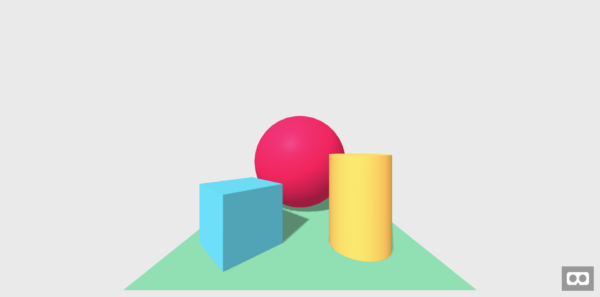
\includegraphics[width=0.7\textwidth]{img/aframe_hello_world.png}
  \caption{Escena básica de A-Frame}
  \label{fig:aframe-basic}
\end{figure}

Una de las principales características de esta tecnología es su arquitectura basada en un modelo de entidad-componente (\textit{Entity Component System}), donde cada objeto dentro de la escena es una entidad que luego es integrada con Three.js para crear la escena.
Una entidad en A-Frame es un objeto HTML que se crea añadiendo la etiqueta \texttt{<a-entity>} y el componente es la apariencia, comportamiento y funcionalidad que se le asigna mediante JavaScript. 

Para hacer uso de un componente se requiere de una serie de pasos previos. Si el componente es externo, es necesario importarlo en la cabecera del HTML, del mismo modo que se importa A-Frame y posteriormente añadirlo a la entidad en la que uno desee usarlo.
Por otra parte, si el componente es de nuestra creación, primero hay que registrar y definir el componente. Esto se hace en un archivo externo de JavaScript mediante el método de \texttt{A-Frame.registerComponente}. A este método, del mimo modo que una función primero se le asigna un nombre, 
este será el nombre del componente. Luego, este método consta de varias funciones internas, las cuales se encargan de definir la apariencia y lógica de dicho componente. Alguna de estas funciones son la función \texttt{schema}, \texttt{init} o \texttt{tick}.
La función \texttt{schema}, define las propiedades principales del componente, estas se pueden modificar dependiendo de la lógica del componente desde el HTML a la hora de llamarlo. La función \texttt{init} se ejecuta una única vez al inicio cuando se inicializa el componente y la función \texttt{tick} se ejecuta a cada frame de la escena.
Una vez el componente está registrado y programado, importamos el archivo que contiene el componente al HTML y lo insertamos a la escena en la entidad u objeto que deseemos. 

Un ejemplo de la llamada de un componente dentro de un archivo de HTML se puede apreciar en \ref{lst:aframe-entity}
\begin{lstlisting}[caption=Ejemplo de llamada de entidad, captionpos=b, label=lst:aframe-entity]
  <html>
    <head>
      <script src="https://aframe.io/releases/1.6.0/aframe.min.js"></script>
      <script src = "componente1.js"></script>
      <script src = "componente2.js"></script>
    </head>
    <body>
      <a-scene>
        <a-entity componente1></a-entity>
        <a-box componente2></a-box>
      </a-scene>
    </body>
  </html>
\end{lstlisting}

En este ejemplo primero se muestra como a una entidad vacía se le añade un componente llamado \texttt{componente 1} y también se muestra como a una entidad de cubo se le añade el componente \texttt{componente 2}.
Del mismo modo, para la creación de un componente, en el archivo \texttt{.js} que posteriormente importaremos en la escena, únicamente es necesario registrar el componente y definir sus características como en el siguiente ejemplo:

\begin{lstlisting}[caption=Ejemplo de creación de entidad, captionpos=b, label=lst:aframe-entity-creation]
  AFRAME.registerComponent('componente1', {
  init() {
    const box = document.createElement('a-box');
    box.setAttribute('position', '-1 0.5 -3');
    box.setAttribute('rotation', '0 45 0');
    box.setAttribute('color', '#4CC3D9');

    const sphere = document.createElement('a-sphere');
    sphere.setAttribute('position', '0 1.25 -5');
    sphere.setAttribute('radius', '1.25');
    sphere.setAttribute('color', '#EF2D5E');

    this.el.appendChild(box);
    this.el.appendChild(sphere);
  }
});
\end{lstlisting}

Este fragmento de código registra el componente \texttt{componente 1} el cual crea un cubo y un cilindro con unos colores, posición y rotación específicos y los añade a la escena.

Para este proyecto, A-Frame ha sido la tecnología principal, permitiendo elementos fundamentales como la creación y gestión de entornos de realidad virtual. 
También, permitió la integración de componentes diseñados mediante JavaScript y permitió el manejo de interacciones más complejas a la vez que optimizaba el rendimiento de la escena 3D.

\subsection{HTML5}
\label{subsec:HTML5}

HTML5 \cite{freeman2018head} es la quinta iteración del lenguaje de HTML (\textit{marcado de hipertexto}), el cual es la estructura básica y principal de toda página web.
Desarrollado conjuntamente por W3C \cite{w3c_mission} (\textit{World Wide Web Consortium}) y WHATWG \cite{whatwg} (\textit{Web Hypertext Application Technology Working Group}).
HTML5 introduce mejoras sustanciales respecto a sus anteriores versiones, incluyendo nuevas etiquetas semánticas, soporte multimedia mejorado y compatibilidad
ampliada con diversos navegadores y dispositivos, dándole mayor flexibilidad y dinamismo a la creación de páginas web.

Una de sus nuevas introducciones clave es la introducción de etiquetas semánticas como: \texttt{<header>}, \texttt{<article>}, \texttt{<section>} y \texttt{<footer>},
que facilitan una estructuración clara y accesible del contenido web. Estas etiquetas no solo ayudan a mejorar la organización de la información, sino que también facilitan la búsqueda
de información por parte de los motores de búsqueda y facilitan la interpretación por parte de los desarrolladores.
Además, HTML5 incorpora nuevas interfaces de programación de aplicaciones (\textit{API}), destacándose las funcionalidades de almacenamiento local mediante
\texttt{localStorage} y \texttt{sessionStorage}, que permiten la gestión eficiente de datos directamente en el navegador, eliminando la necesidad de bases de datos externas.

HTML5 también introduce mejoras significativas en la gestión de contenido multimedia, eliminando la necesidad de complementos externos. Para esto se implementaron
las etiquetas \texttt{<audio>} y \texttt{<video>} las cuales permiten la incorporación directa de archivos de sonido y video en las páginas web, permitiendo mayor dinamismo en el desarrollo.
Otro elemento que se añadió fue el elemento \texttt{<canvas>} el cual habilita la generación de gráficos y animaciones en tiempo real a través de JavaScript, permitiendo el desarrollo de aplicaciones interactivas y videojuegos en línea.

HTML5 se ha establecido firmemente como un estándar en el desarrollo de aplicaciones web progresivas (\textit{PWA}) y en entornos multiplataforma. Su integración con tecnologías como CSS3 y JavaScript
permite la creación de interfaces dinámicas y adaptativas, compatibles con una amplia gama de dispositivos, desde ordenadores hasta tabletas y teléfonos.

Gracias a que HTML es una tecnología extensible, tecnologías como A-Frame o WebXR han sido posibles de utilizar, ya que son extensiones de HTML. WebXR permitió poder trabajar con entornos VR desde el navegador, mientras que A-Frame fue el eje central 
del proyecto, donde se estructuró la escena. HTML fue una de las tecnologías más importantes, puesto que ofrece una estructura esencial para el desarrollo del proyecto, haciendo uso de sus extensiones de A-Frame y WebXR para poder mostrar los elementos de la escena en la realidad virtual.

\subsection{JavaScript}
\label{subsec:JavaScript}
JavaScript \cite{mdn2024} es un lenguaje de programación ligero y multiplataforma utilizado principalmente para la creación de contenido dinámico e interactivo para páginas web.
Su flexibilidad permite desarrollar elementos para mejorar la interacción del usuario en páginas web tanto del lado del servidor como del lado del cliente. En 1997, JavaScript fue estandarizado
por \textit{ECMA} como ECMAScript y poco después como un estándar \textit{ISO}.

JavaScript, creado por Brendan Eich de Netscape en 1995 bajo el nombre de \textit{Mocha}, posteriormente se renombró a LiveScript y finalmente a JavaScript.
En el año 2000, JavaScript se extendió al lado de los servidores con la introducción de tecnologías como \textit{Node.js}, y posteriormente su popularidad creció con la llegada de \textit{AJAX}. Y Con la llegada de ECMAScript 6 en 2015, se introdujeron características más avanzadas y
actualizaciones anuales, haciendo que hoy en día sea uno de los lenguajes más importantes en el desarrollo web.

JavaScript es un lenguaje de programación de alto nivel, lo que significa que su lenguaje está diseñado para ser lo más 'humano' posible, permitiendo una rápida comprensión del código sin necesidad de un nivel alto de conocimientos.
Es un lenguaje basado en eventos, ya sean entradas de ratón o entradas de teclado, permitiendo la creación de interfaces de usuario interactivas. JavaScript puede integrarse en un HTML dentro de la etiqueta \texttt{<script>} de forma directa, escribiendo el código.
También, se puede introducir códigos de JavaScript, los cuales estén en archivos distintos con la extensión correspondiente al lenguaje (.js), esto es posible vinculando dicho archivo en la cabecera del HTML.

Para este proyecto formo un papel crucial, ya que fue con JavaScript que se desarrollaron los distintos componentes de A-Frame que se usaron para el funcionamiento del proyecto. Permitió diseñar e implementar la lógica que hay tras cada componente, permitiendo alcanzar los resultados obtenidos.

\subsection{Three.js}
\label{subsec:Threejs}

Three.js \cite{dirksen2015} es una biblioteca de código abierto de JavaScript utilizada para la creación de gráficos 3D en los navegadores web. Three.js funciona sobre WebGL, la cual permite generar y visualizar animaciones y escenas 3D en el navegador sin necesidad de complementos. La tecnología de WebGL también puede usarse junto con el elemento \texttt{<canvas>} de HTML.

Esta biblioteca proporciona una API de alto nivel la cual permite al usuario la creación y manipulación de geometrías 3D como cubos, esfera o planos, así como la aplicación de texturas o la aplicación de tanto cámaras como de efectos de iluminación en las escenas, permitiendo que el desarrollo de dichas escenas sea mucho más simplificado. 
También, Three.js permite la posibilidad de importar modelos 3D desde archivos distintos creados desde aplicaciones distintas.

La biblioteca de Three.js ofrece una alta variedad de herramientas que permiten la gestión y control de usuario, facilitando así tanto la navegación como la interacción dentro de las escenas 3D. También, Three.js soporta animaciones suaves y dinámicas tanto para objetos en la escena como para cámaras, lo cual permite la creación de efectos visuales más dinámicos e impresionantes, al igual que juegos interactivos. 

Gracias a la amplia variedad de posibilidades que permite la biblioteca de Three.js, las opciones de los elementos o escenas que se pueden llegar a crear son básicamente ilimitadas. Siendo capaz de generar escenas complejas como la de la figura \ref{fig:three}
\begin{figure}[H] 
  \centering
  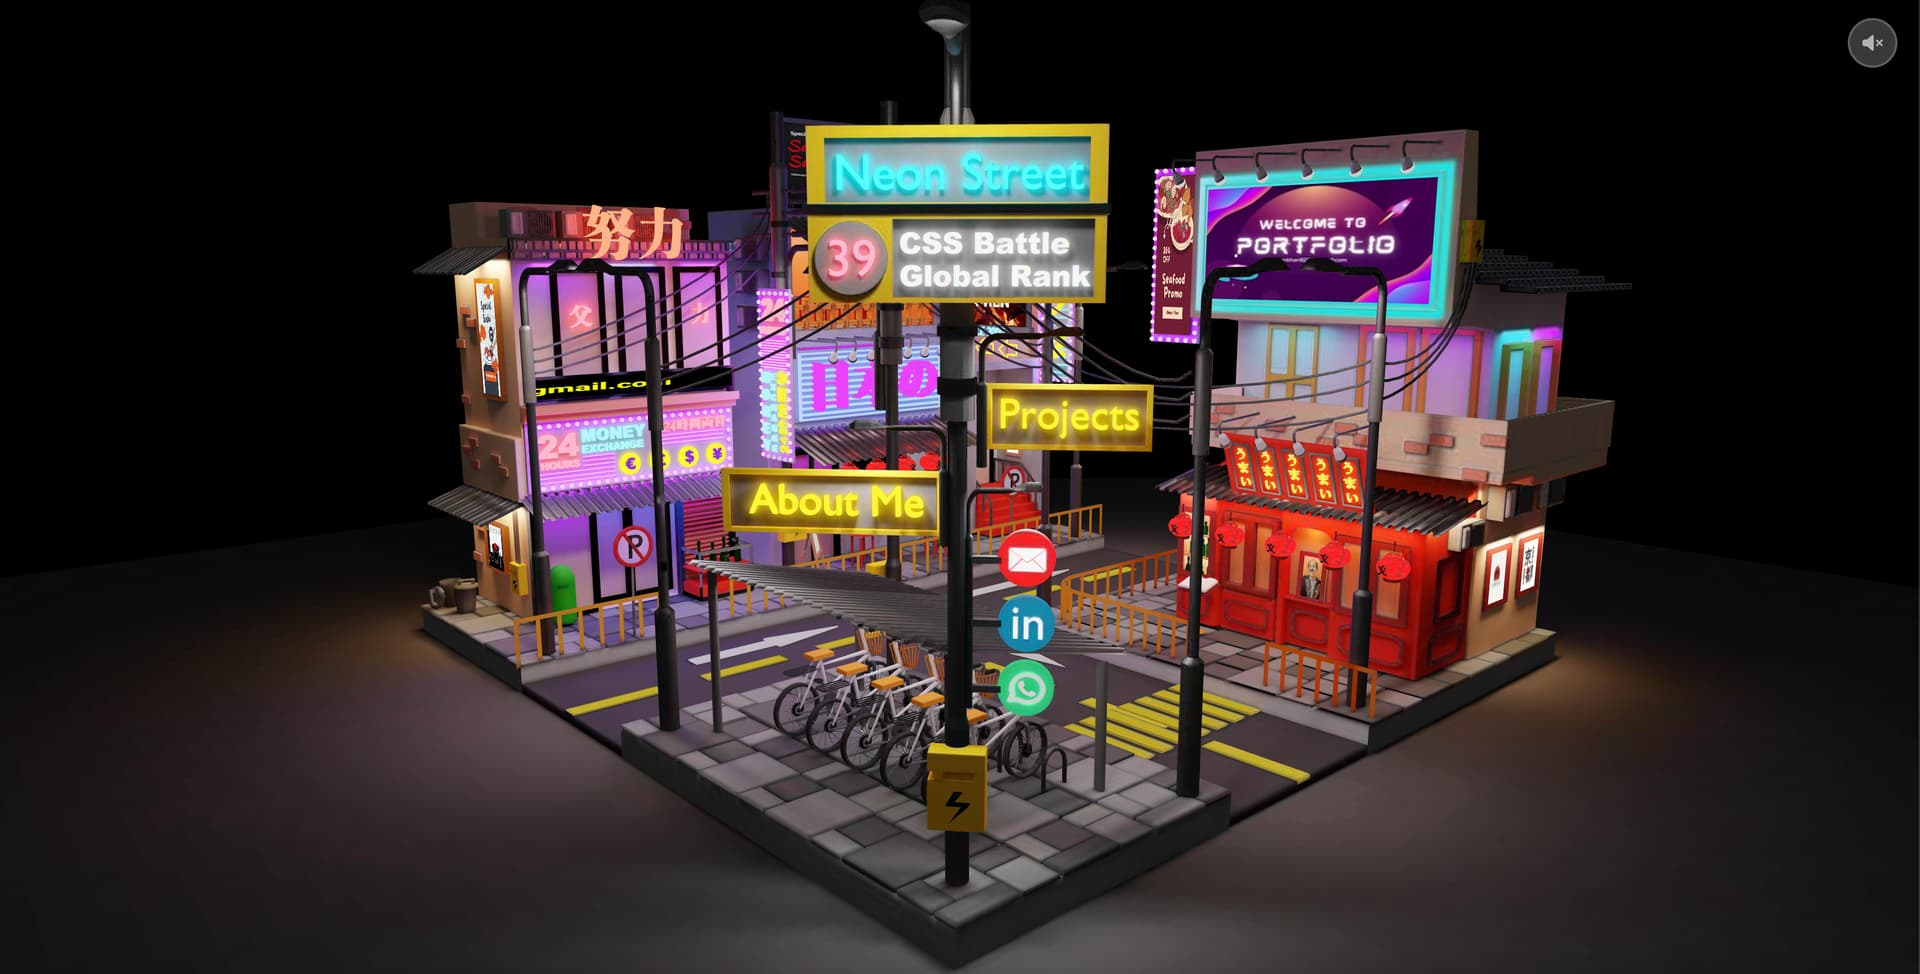
\includegraphics[width=0.7\textwidth]{img/three.jpeg}
  \caption{Escena creada con Three.js}
  \label{fig:three}
\end{figure}

Three.js permitió añadir una capa más simplificada a WebGL, simplificando así el proceso de creación y manipulación de los elementos 3D. Permitió generar un entorno 3D con mayor dinamismo y control para el proyecto.

\subsection{WebXR}
\label{subsec:WebXR}

WebXR \cite{onirix2024} es una tecnología desarrollada por W3C (\textit{World Wide Web Consortium}) que permite crear experiencias inmersivas desde el navegador. Esta tecnología combina la Realidad Aumentada (\textit{AR}) y la Realidad Virtual (\textit{VR}) con la accesibilidad de un navegador web.
Lo cual permite a los usuarios experimentar e interactuar con entornos tridimensionales a través de cualquier dispositivo con acceso a un navegador compatible.

A medida que la tecnología de WebXR ha ido evolucionando, se han desarrollado distintos tipos de experiencias para poder adaptarse a distintos contextos y necesidades. Hoy en día, se podría clasificar los distintos tipos en 3 categorías:
\begin{itemize}
  \item \textbf{WebXR AR:} Este tipo de WebXR combina el mundo virtual y el mundo real, permitiendo que distintos elementos del mundo virtual puedan superponerse en el entorno físico a través
        de la cámara de un dispositivo compatible, pero sin que llegue a influir el mundo real en los elementos virtuales.
  \item \textbf{WebXR VR:} Este modo permite a los usuarios sumergirse en el entorno virtual creado, y con la ayuda de dispositivos suplementarios como auriculares, la experiencia es aún mayor. Esta tecnología permite a los usuarios
        interactuar y experimentar en primera persona distintos entornos virtuales, desde juegos y entretenimiento, hasta simulaciones virtuales y visualizaciones en 3D.
  \item \textbf{WebXR MR(Mixed Reality):} Esta tecnología combina el mundo real y el virtual de forma más profunda que la tecnología AR. Permite a los usuarios poder interactuar con elementos tantos virtuales como físicos y que estos puedan interactuar entre sí. Este tipo de combinación proporciona un nivel mayor de interacción entre el usuario y
        y su entorno, dando mayor número de posibilidades para la creación de contenido.
\end{itemize}

Estos distintos tipos de WebXR ofrecen distintos tipos de experiencias dependiendo del entorno virtual que se quiera diseñar.

Fue gracias a WebXR, que en este proyecto se pudieron realizar las distintas escenas inmersivas que permitieron ir comprobando el avance del proyecto con cada una de las demos que se creaban y que posteriormente se explicaran, el uso de su API \cite{w3c2024} fue parte fundamental, en especial la parte relacionada con el seguimiento de manos \cite{w3cHandInput2024}. Además de eso, fue gracias a WebXR que se pudo realizar la detección de las manos, ya que ya posee una función integrada que permite el handtracking y al querer trabajar sobre el navegador era la mejor opción para ello. 

\subsection{WebGL}
\label{subsec:WebGL}
WebGL \cite{webgl_encodebiz} \cite{matsuda2013} (\textit{Web graphics Library}), se trata de una tecnología de bajo nivel multiplataforma usada para la renderización de gráficos tanto tridimensionales como bidimensionales dentro de cualquier navegador que sea compatible.

WebGL fue lanzado en 2011 por el grupo \textit{Khronos}\footnote{\url{https://www.khronos.org/about/}}. Esta tecnología se fundamenta en OpenGL ES, la cual es una variante simplificada de OpenGL, diseñada para dispositivos móviles. WebGL ha sufrido numerables actualizaciones, 
lo cual ha permitido una evolución continua que ha ido mejorando tanto su funcionalidad como compatibilidad tanto en navegadores de escritorio como en navegadores en dispositivos móviles. 

WebGL está diseñado para trabajar directamente con la GPU (\textit{Graphic Processing Unit}) del dispositivo, lo cual permite un mayor aprovechamiento de la computación para poder generar gráficos detallados y de alta calidad. 
Además, la tecnología de WebGL está diseñada para poder integrarse de manera fluida con otros estándares de desarrollo web como HTML, CSS o DOM. 

Gracias a esta tecnología fue posible renderizar en la escena las distintas entidades que forman las manos del mismo modo que las otras entidades que se crearon para ir comprobando si los componentes creados funcionaban.

\section{Tecnologias auxiliares}
\label{sec:tecnologias-auxiliares}
En esta sección se detallan y describen las distintas tecnologías que, aunque no hayan influido de manera directa en los resultados del proyecto, han tenido un papel crucial para el desarrollo de este.
Entre dichas tecnologías se encuentra el \textit{IDE} utilizado durante el proyecto, al igual que el dispositivo utilizado para realizar las pruebas de las demos, la plataforma donde se almacenó el código y también el software utilizado para la redacción de esta memoria.

\subsection{Visual Studio Code}
\label{subsec: visualstudiocode}

\textit{Visual Studio Code}\footnote{\url{https://code.visualstudio.com/docs}} (\textit{VS Code}) es un potente entorno de desarrollo integrado (\textit{IDE}) el cual está disponible para Windows, Linux, MacOS y versión web. VS Code es una de las plataformas de edición de código más utilizadas a nivel mundial 
por toda clase de desarrolladores de software debido a su versatilidad, flexibilidad y amplia gama de extensiones que facilitan la edición y depuración de código.

Una de las pestañas más importantes durante el desarrollo fue su pestaña de \textbf{Source Control}, la cual luego de conectar mi repositorio de GitHub, permite ir guardando el código en GitHub para tener un control de las distintas versiones del código. 

Gracias a las numerosas extensiones que hay disponibles, facilitan en gran medida la creación y depuración de código, permitiendo cosas como autocompletar palabras o expresiones o permitir compilar o depurar con algún lenguaje que VS Code no tenga por defecto.
Algunas de las extensiones utilizadas en este proyecto han sido: 
\begin{itemize}
  \item \textbf{A-Frame completition}: Permite autocompletar rápidamente a la hora de escribir los distintos elementos o Snippets que posee A-Frame
  \item \textbf{Error lens}: A la hora de depuración, permite visualizar dentro del código si hay algún error de sintaxis o lógica 
  \item \textbf{LaTeX Workshop}: Permite la escritura, compilación y previsualización de la memoria de este proyecto.
\end{itemize}

\subsection{GitHub}
\label{subsect:github}

\textit{GitHub}\footnote{\url{https://github.com/about}} es una plataforma basada en la nube que permite almacenar distintos repositorios y en cada repositorio código. GitHub está basado en Git \cite{git}, el cual fue creado en 2005 por Linus Torvalds como un sistema de control de versiones de código abierto.
Este sistema fue desarrollado con la intención de ayudar a los desarrolladores a tener en cualquier dispositivo con acceso a internet todo el historial de código que están desarrollando. 

Esta tecnología es ampliamente utilizada a nivel mundial por desarrolladores de todo tipo debido a su capacidad de almacenar, soportar y gestionar proyectos de toda clase. Una de las funciones clave que presenta la plataforma, es la capacidad de crear ramificaciones (branches). Esta opción permite a los desarrolladores poder generar copias del código del repositorio en el que 
están trabajando para poder trabajar en paralelo y posteriormente poder integrar los cambios realizados en paralelo al código principal. Esta opción también permite que más de un desarrollador pueda trabajar en el mismo código, haciendo que cada uno trabaje en paralelo en ramas distintas. 

GitHub aprovecha todas las ventajas que permite Git, permitiendo crear repositorios en la nube para sus proyectos Git, que los desarrolladores pueden llegar a compartir con otras personas. Esta plataforma también facilita la colaboración entre desarrolladores y aparte de las ventajas ya mencionadas de Git permite también el uso de herramientas de gestión de proyectos, al igual que acciones automáticas. 

Durante este proyecto se creó el repositorio de GitHub \textit{TFG}\footnote{\url{https://github.com/JuJoarias/TFG}} donde se fue guardando todas las versiones del código al igual que todas las demos y pruebas realizadas.

\subsection{Meta Quest 3}
\label{subsec:metaquest}

Meta Quest se trata de un dispositivo inalámbrico diseñado para disfrutar de contenido de realidad virtual (VR) por \textit{Meta}\footnote{\url{https://www.meta.com/es-es/about/company-info/}} \cite{meta_company_info}. Dicho dispositivo está compuesto por unas gafas, un micrófono y auriculares integrados en un único dispositivo que el usuario pone en su cabeza y un par de mandos inalámbricos. 
La primera versión fue lanzada en 2020 con las Meta Quest 2 y 3 años más tarde, en 2023, se lanzaron las \textit{Meta Quest 3}\footnote{\url{https://en.wikipedia.org/wiki/Meta_Quest_3}}. 

Para este proyecto se han utilizado unas Meta Quest 3, las cuales contaban con una memoria de 8 GBB de memoria RAM, una resolución de 2064x2208 píxeles por cada uno de los ojos. También, cuenta con mejoras respecto al campo de visión (FOV) respecto a su versión anterior. Para este proyecto jugaron un papel crucial, ya que al enfocarse en la detección de mandos
el proyecto, sin las gafas, no se habría podido probar los resultados que se iban obteniendo.

\begin{figure}[H] 
  \centering
  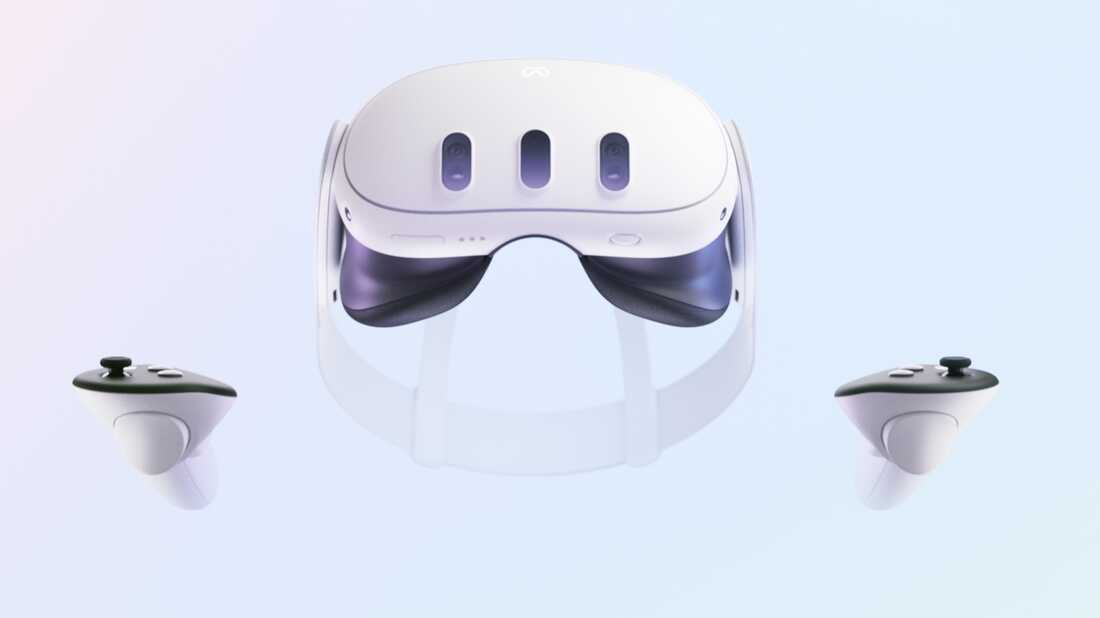
\includegraphics[width=0.7\textwidth]{img/meta_quest.jpg}
  \caption{Meta Quest 3}
  \label{fig:metaquest}
\end{figure}

\subsection{LaTeX}
\label{subsec:latex}

\textit{LaTeX}\footnote{\url{https://www.latex-project.org}} \cite{mittelbach2004latex} es un software de uso libre de creación de documentación de alta calidad. Este sistema es altamente utilizado para la creación de documentación técnica o científica de media o larga extensión, aunque gracias a su versatilidad se puede utilizar para cualquier tipo de documentación.

Entre las distintas características de LaTeX cabe destacar su capacidad de manejar expresiones matemáticas complejas, lo cual es una herramienta indispensable para cualquier documento científico. También gracias a su software motor TeX LaTeX es capaz de convertir los comandos de texto, utilizados para expresar los resultados tipográficos, en un archivo PDF profesional. 

Además de facilitar la creación de fórmulas matemáticas complejas, LaTeX también ofrece otras facilidades avanzadas, como puede ser la creación de un índice del contenido, un índice de las figuras utilizadas, gestión de bibliografías o referencias simplificando la organización del documento y la citación de figuras o elementos externos en la bibliografía.

Para este proyecto, LaTeX facilito considerablemente el trabajo a la hora de crear este documento, ayudando con la creación y gestión de índices, imágenes y bibliografía, al igual que a estructurar el texto del documento de forma correcta.

%%%%%%%%%%%%%%%%%%%%%%%%%%%%%%%%%%%%%%%%%%%%%%%%%%%%%%%%%%%%%%%%%%%%%%%%%%%%%%%%
%%%%%%%%%%%%%%%%%%%%%%%%%%%%%%%%%%%%%%%%%%%%%%%%%%%%%%%%%%%%%%%%%%%%%%%%%%%%%%%%
% RESULTADOS capitulo 3%
%%%%%%%%%%%%%%%%%%%%%%%%%%%%%%%%%%%%%%%%%%%%%%%%%%%%%%%%%%%%%%%%%%%%%%%%%%%%%%%%

\cleardoublepage
\chapter{Descripción de los resultados obtenidos}
\label{chap:resultados}
En este capítulo se describe en detalle los resultados obtenidos al final de este proyecto. Primero se dará una descripción funcional para el usuario, donde se describirá las posibles aplicaciones funcionales de este proyecto, además de una descripción de la escena, donde se detallarán los detalles de esta para que cualquier usuario pueda manejarse en esta. También, se describen los detalles técnicos detrás del funcionamiento del proyecto y su implementación,
dando detalles en profundidad sobre la estructura de los componentes y su utilización.

\section{Descripción funcional para el usuario}
\label{sec:manual-usuario}
El proyecto se plantea como una 'caja de herramientas', la cual consiste en una serie de componentes que permiten utilizar las manos dentro de las escenas virtuales dentro de un navegador. El proyecto está dividido en dos áreas principales, la primera se centra en las entidades comunes de una escena de A-Frame, como cubos y esferas. El enfoque de esta área consiste en la creación e implementación de componentes que nos permitan interactuar con las distintas entidades dentro de la escena de forma más natural, permitiendo coger y mover dichos elementos entre otras acciones mediante el uso de gestos con nuestras manos.

La segunda área del proyecto se centra en el uso avanzado del sistema de seguimiento de manos que posee WebXR, permitiendo la detección y el renderizado de las manos dentro del entorno virtual. Aparte de la detección, esta área también se centra en la creación de la lógica necesaria para que las manos puedan interactuar con los distintos elementos dentro del entorno virtual, mediante la detección de gestos.

Los componentes diseñados en este proyecto, tanto en la primera área como en la segunda, permiten al usuario poder visualizar sus manos dentro del entorno virtual además de poder interactuar con los distintos elementos de la escena, permitiendo acciones como agarrar, estirar o hacer click sobre dichos elementos. Esto permite la creación de escenas o aplicaciones dentro del navegador que permitan al usuario utilizar sus propias manos dentro de la escena para interactuar de diversas maneras con dicha escena. 

Para mostrar los resultados obtenidos de este proyecto se crearon un total de tres escenas:
\begin{itemize}
  \item Demo componentes
  \item Demo juego click
  \item Demo dibujar
\end{itemize}

La primera escena es la más sencilla de las tres, en ella, se muestra cada uno de los componentes desarrollados de forma directa, mientras que las otras dos escenas, son ejemplos aplicados de dichos componentes.

Si el usuario se encuentra en un ordenador, ninguna de las tres escenas funcionaría. Al cargar la página web correspondiente a cada una se puede visualizar la escena y es posible moverse usando el ratón y las teclas de flechas o las teclas 'ASDW', pero sí se intenta entrar al modo VR,
el usuario sería incapaz de moverse o de hacer cualquier cosa, únicamente funcionan mediante el uso de un dispositivo VR como lo es las Quest3 que se usaron en este proyecto. Además, a las tres escenas se les ha añadido el componente \textit{environment}\footnote{\url{https://github.com/supermedium/aframe-environment-component}} para mostrar que los componentes creados en este proyecto son compatibles con componentes nativos.

\subsection{Demo Componentes}
\label{subsec:demo-componentes}
Nada más cargar la escena de la \textit{demo componentes}\footnote{\url{https://github.com/JuJoarias/TFG/blob/main/demo/demo.html}}, el usuario se encontrará en el centro de esta, rodeado de una serie de cubos que están sobre unos pedestales y cada uno posee un panel encima de estos. Cinco de los cubos (los cuales se encuentran formando un semicírculo frente al usuario) representan cada uno de los distintos componentes de interacción que se crearon durante el proyecto y detrás del usuario hay un sexto cubo, el cual posee todos los componentes para así poder probarlos todos sin necesidad de interactuar con todos los otros cubos.

Al principio, si el sistema no ha detectado las manos, en el centro de la escena aparecerá una esfera, pero dicha esfera desaparece en cuanto el sistema detecta las manos. Es recomendable que lo primero en hacer al cargar la escena es que el usuario se mire las manos para poder detectarlas y renderizarlas correctamente. 

Una vez se detectan las manos, manos, el usuario puede acercarse a cada uno de los cubos. Encima de cada cubo hay un panel flotante, donde aparece el nombre del componente que posee el cubo en cuestión al igual que una descripción de la acción necesaria para interactuar con el cubo en cuestión, esta descripción contiene tanto el gesto necesario para poder interactuar con el cubo como el movimiento de mano/s si es necesario. 

La mayoría de los cubos requieren que el usuario se acerque a estos y que los toque dentro de la escena virtual para poder interactuar con ellos, en caso de que el espacio donde se encuentra el usuario no sea lo bastante grande como para acercarse a todos los cubos individualmente, detrás del usuario al aparecer se encuentra un único cubo que posee todos los componentes, así el usuario puede probar todas las funcionalidades sin necesidad de ir uno por uno. 
Para poder interactuar con los distintos cubos, el usuario necesita realizar dos tipos de gestos, el primero es el gesto \texttt{Pinch}, este gesto es necesario para la mayoría de los cubos, y todos los cubos que requieren de este gesto es necesario acercarse a ellos para poder interactuar. Y el segundo es el gesto \texttt{Point}, los cubos que requieren de este segundo gesto no es necesario acercarse hasta estos para interactuar con ellos, si se realiza el gesto correctamente y hay una línea directa de visión entre el usuario y el cubo es posible interactuar con él desde cualquier parte de la escena. 
En la figura \ref{fig:demo_componentes} se puede apreciar lo primero que ve el usuario al entrar en la escena.

Los distintos componentes representados son aquellos que se han desarrollado en este proyecto, siendo estos: 
\begin{itemize}
  \item Componente drag
  \item Componente stretch
  \item Componente slide
  \item Componente hoover
  \item Componente clickable
\end{itemize}

\begin{figure}[H] 
  \centering
  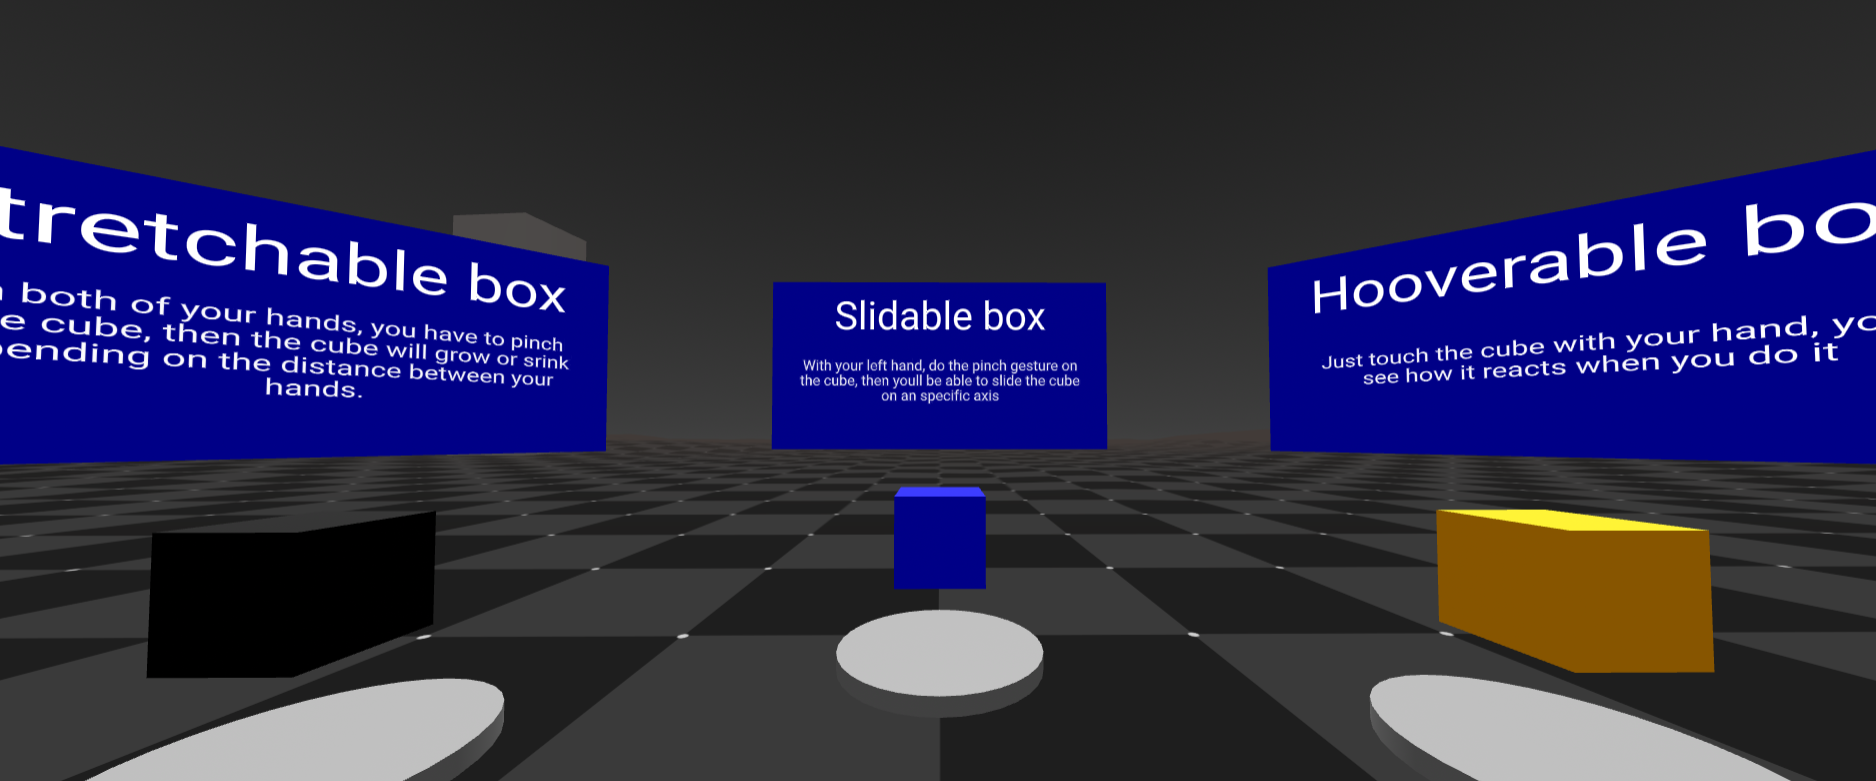
\includegraphics[width=0.7\textwidth]{img/demo_componentes.png} 
  % \fbox{\rule{0pt}{150pt} \rule{0.7\textwidth}{0pt}} 
  \caption{Escena Demo Componentes}
  \label{fig:demo_componentes}
\end{figure}

\subsection{Demo Juego Clicks}
\label{subsec:demo-juego}
Esta demo de \textit{juego clicks}\footnote{\url{https://github.com/JuJoarias/TFG/blob/main/demo/juego_click.html}}, tal y como su nombre indica, se trata de un pequeño juego en el que el usuario tiene que disparar una serie de cubos que se generan de forma aleatoria al rededor del usuario, mediante el uso del gesto \texttt{Point}. 

Para la creación de esta demo, se hizo uso del componente \texttt{clickable}. Dicho componente únicamente fue modificado para que en vez de cambiar el color del elemento al recibir el click, lo eliminase de la escena y sumara a la puntuación del juego. También, se creo un componente encargado de crear los cubos de forma aleatoria al rededor del usuario y sé 
implemento una cuenta atrás y puntuación. Al cargar la escena, como se aprecia en la figura \ref{fig:demo_juego_antes}, el usuario verá un panel el cual es necesario disparar para que empiece el juego.

\begin{figure}[H] 
  \centering
  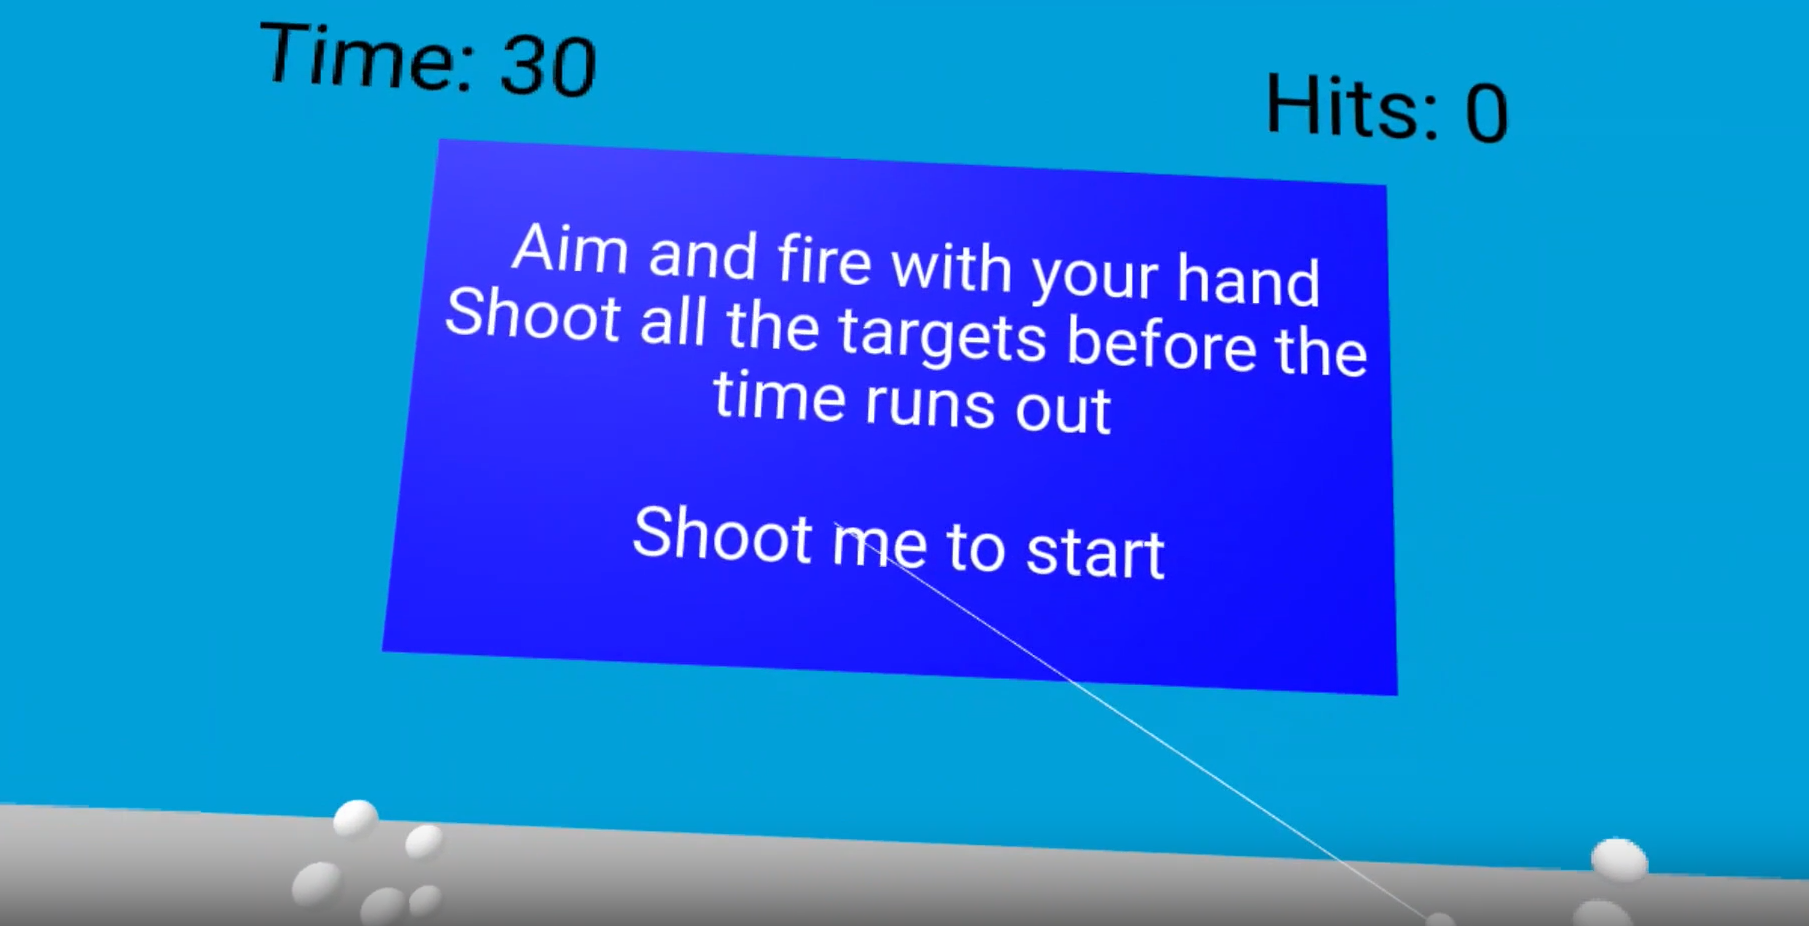
\includegraphics[width=0.7\textwidth]{img/demo_juego_antes.png} 
  % \fbox{\rule{0pt}{150pt} \rule{0.7\textwidth}{0pt}} 
  \caption{Escena Demo Juego Clicks al iniciar}
  \label{fig:demo_juego_antes}
\end{figure}

Una vez se inicia el juego, se generan los cubos y se inicia la cuenta atrás. Para eliminar los cubos es necesario dispararlos mediante el uso del gesto \texttt{Point} antes de que se acabe el tiempo. En la figura \ref{fig:demo_juego_despues} se muestra una escena con el juego ya empezado.

\begin{figure}[H] 
  \centering
  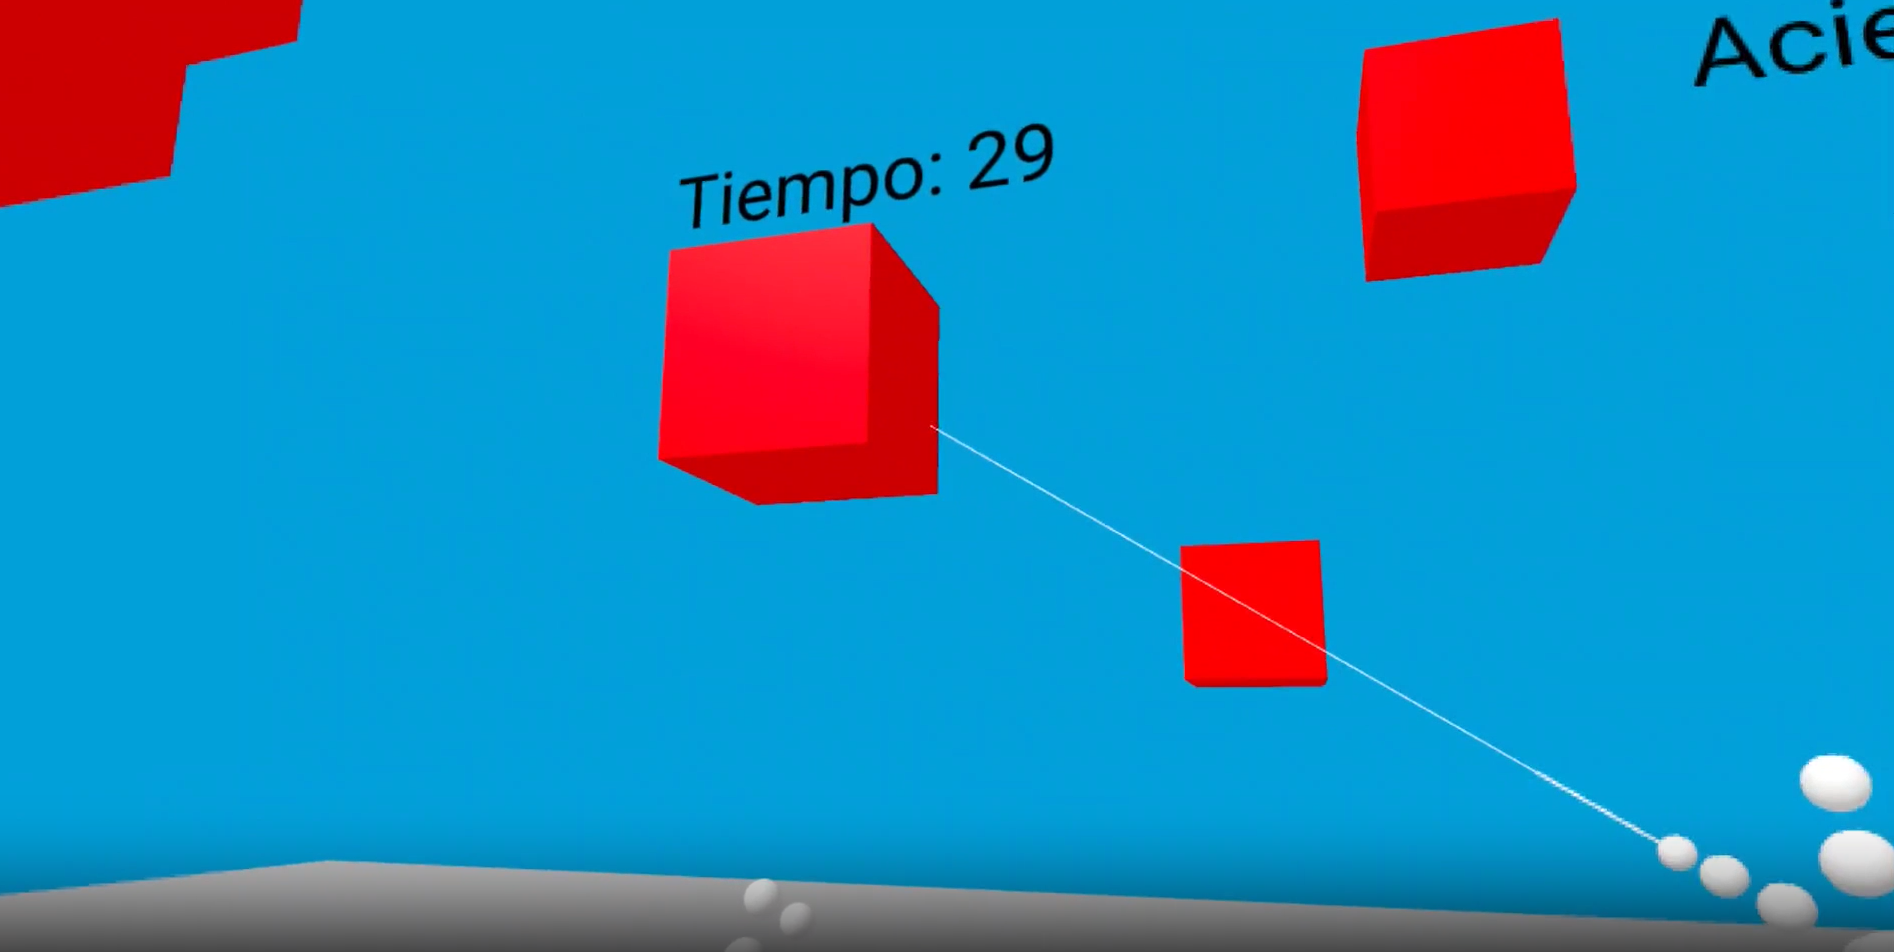
\includegraphics[width=0.7\textwidth]{img/demo_juego_despues.png} 
  % \fbox{\rule{0pt}{150pt} \rule{0.7\textwidth}{0pt}} 
  \caption{Escena Demo Juego Clicks juego iniciado}
  \label{fig:demo_juego_despues}
\end{figure}

\subsection{Demo Dibujar}
\label{subsec:demo-dibujar}
Para la demo \textit{dibujar}\footnote{\url{https://github.com/JuJoarias/TFG/blob/main/demo/dibujar.html}}, se emplean los componentes \texttt{drag} y \texttt{hoover}. En esta escena el usuario tendrá frente a el un cilindro al cargar la escena, dicho cilindro será el bolígrafo. En cuanto el usuario tome el bolígrafo 
mediante el uso del gesto \texttt{Pinch}, en la punta de este, se empieza a dibujar una serie de esferas de color, dejando un rastro por donde pasamos el bolígrafo.

Para ello, al componente \texttt{drag} se le ha añadido una función encargada de dibujar las esferas de color cada 20 ms, el resto del funcionamiento del componente permanece igual que antes.
En la figura \ref{fig:demo_dibujar_antes} se muestra lo que ve el usuario al iniciar la escena y en la figura \ref{fig:demo_dibujar_despues} se muestra como el usuario usa el bolígrafo para dibujar.

\begin{figure}[H] 
  \centering
  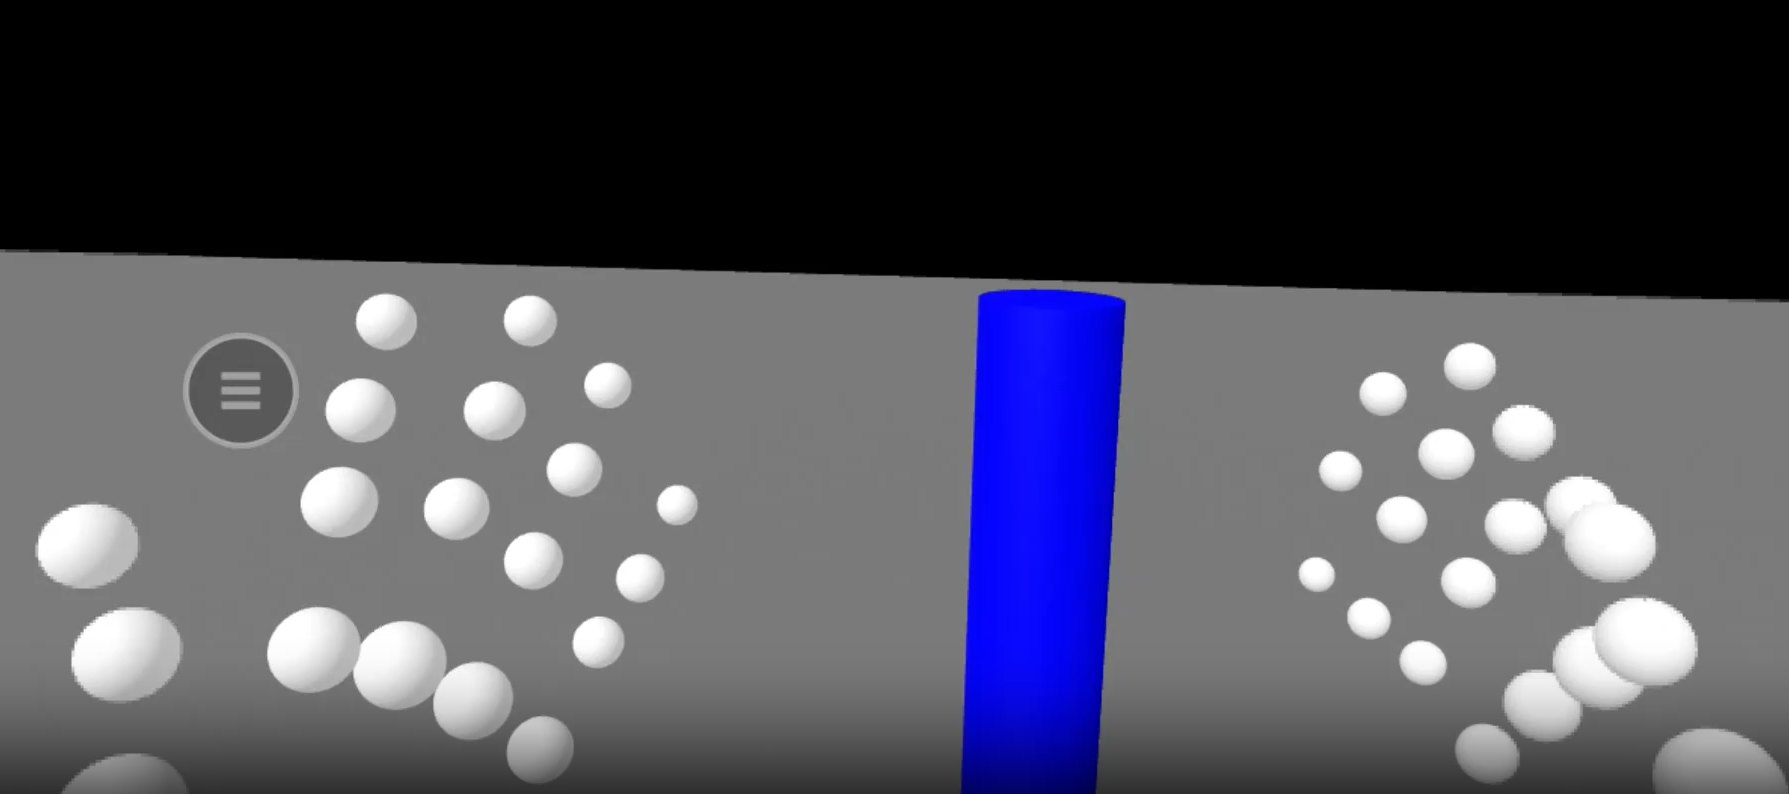
\includegraphics[width=0.7\textwidth]{img/demo_dibujar_antes.png} 
  % \fbox{\rule{0pt}{150pt} \rule{0.7\textwidth}{0pt}} 
  \caption{Escena Demo Dibujar inicio}
  \label{fig:demo_dibujar_antes}
\end{figure}

\begin{figure}[H] 
  \centering
  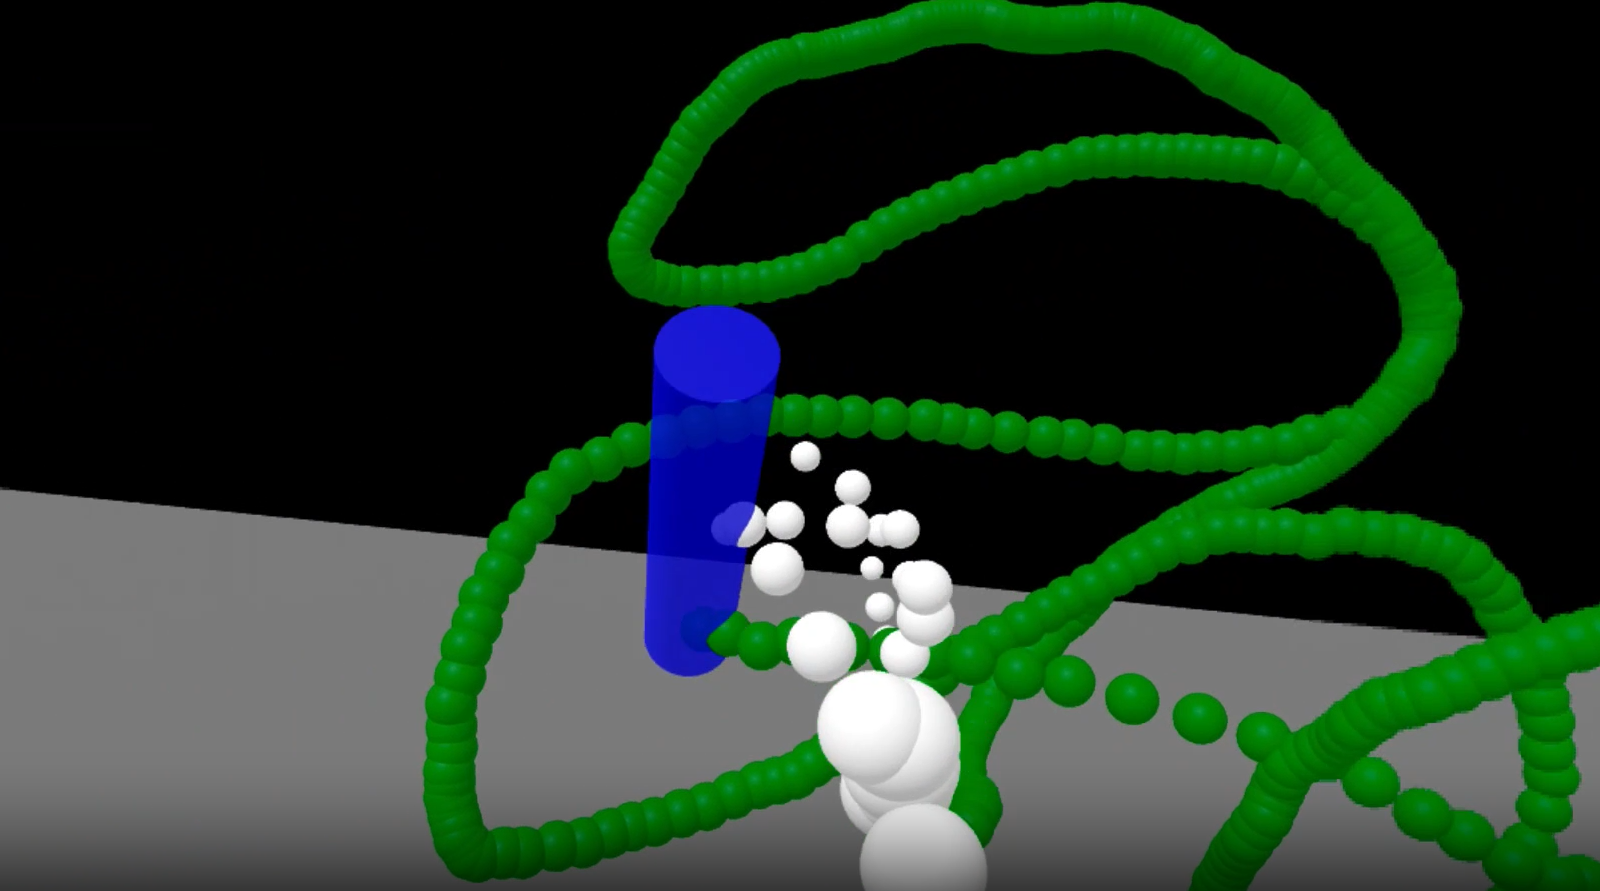
\includegraphics[width=0.7\textwidth]{img/demo_dibujar_despues.png} 
  % \fbox{\rule{0pt}{150pt} \rule{0.7\textwidth}{0pt}} 
  \caption{Escena Demo Dibujar}
  \label{fig:demo_dibujar_despues}
\end{figure}

\section{Descripción tecnica}
\label{sec:descripcion-tecnica}

Para esta sección hablaremos de las dos partes principales del proyecto, la detección e implementación de las manos en el entorno virtual y la creación de los distintos componentes que acompañan a los elementos de la escena para interactuar con ellos.

\subsection{Seguimiento de manos}
\label{subsec:handtracking}
La detección de las manos es uno de los pilares fundamentales de este proyecto. El proceso siguió varias etapas hasta llegar al resultado final de este proyecto. Para crear el componente de detección y renderización de manos se hizo uso de la tecnología WebXR, y dado que el proyecto entero se hizo usando A-Frame, este proyecto únicamente funciona en navegadores compatibles con WebGL, en especial, los navegadores de los dispositivos VR, son los únicos en los que funciona, ya que sin un dispositivo VR, es imposible detectar las manos, con lo cual, la escena no funcionaría.

Como ya se ha mencionado, este proyecto hizo uso de WebXR, esta tecnología fue indispensable para realizar la detección de las manos. Para empezar, había que definir dentro de la escena, en el HTML, que se iba a usar dicha tecnología tal y como se muestra en el fragmento de código \ref{lst:webxr}. Ya con eso, desde el archivo JavaScript donde se definían los componentes se podía acceder a su información. Para ello, primero era necesario acceder a la sesión XR y posteriormente a la información de los inputs, las manos, en el fragmento de código \ref{lst:defXR} se muestra de manera simplificada como acceder a dicha información.

\begin{lstlisting}[caption=Definición de WebXR en la escena, captionpos=b, label=lst:webxr]
  xr-mode-ui="enabled: true; enterVRDisabled: false;" 
  webxr="optionalFeatures: hand-tracking"
\end{lstlisting}

En el siguiente ejemplo, en el fragmento de código \ref{lst:defXR}, se accede a la información de los inputs, ambas manos, y se obtiene la información de la posición de la punta del dedo índice para luego guardarlo en una variable. Siguiendo este concepto fue que se pudo obtener toda la información necesaria de las manos para toda la parte relacionada con el seguimiento de manos.

\begin{lstlisting}[caption=Ejemplo simplificado de acceder a la información XR, captionpos=b, label=lst:defXR]
  const session = this.el.sceneEl.renderer.xr.getSession();
  const inputSources = session.inputSources;
  for (const inputSource of inputSources) {
    const hand = inputSource.hand;
    
    const indexTip = hand.get('index-finger-tip');
    if (indexTip) {
      const pose = frame.getJointPose(indexTip, referenceSpace);
    }
  }
\end{lstlisting}


Primero, se creó el componente de \texttt{manos}, este componente era el encargado de detectar y renderizar las manos dentro de la escena virtual. En la figura \ref{fig:manos} se aprecia el resultado de las manos dentro de la escena.

\begin{figure}[H] 
  \centering
  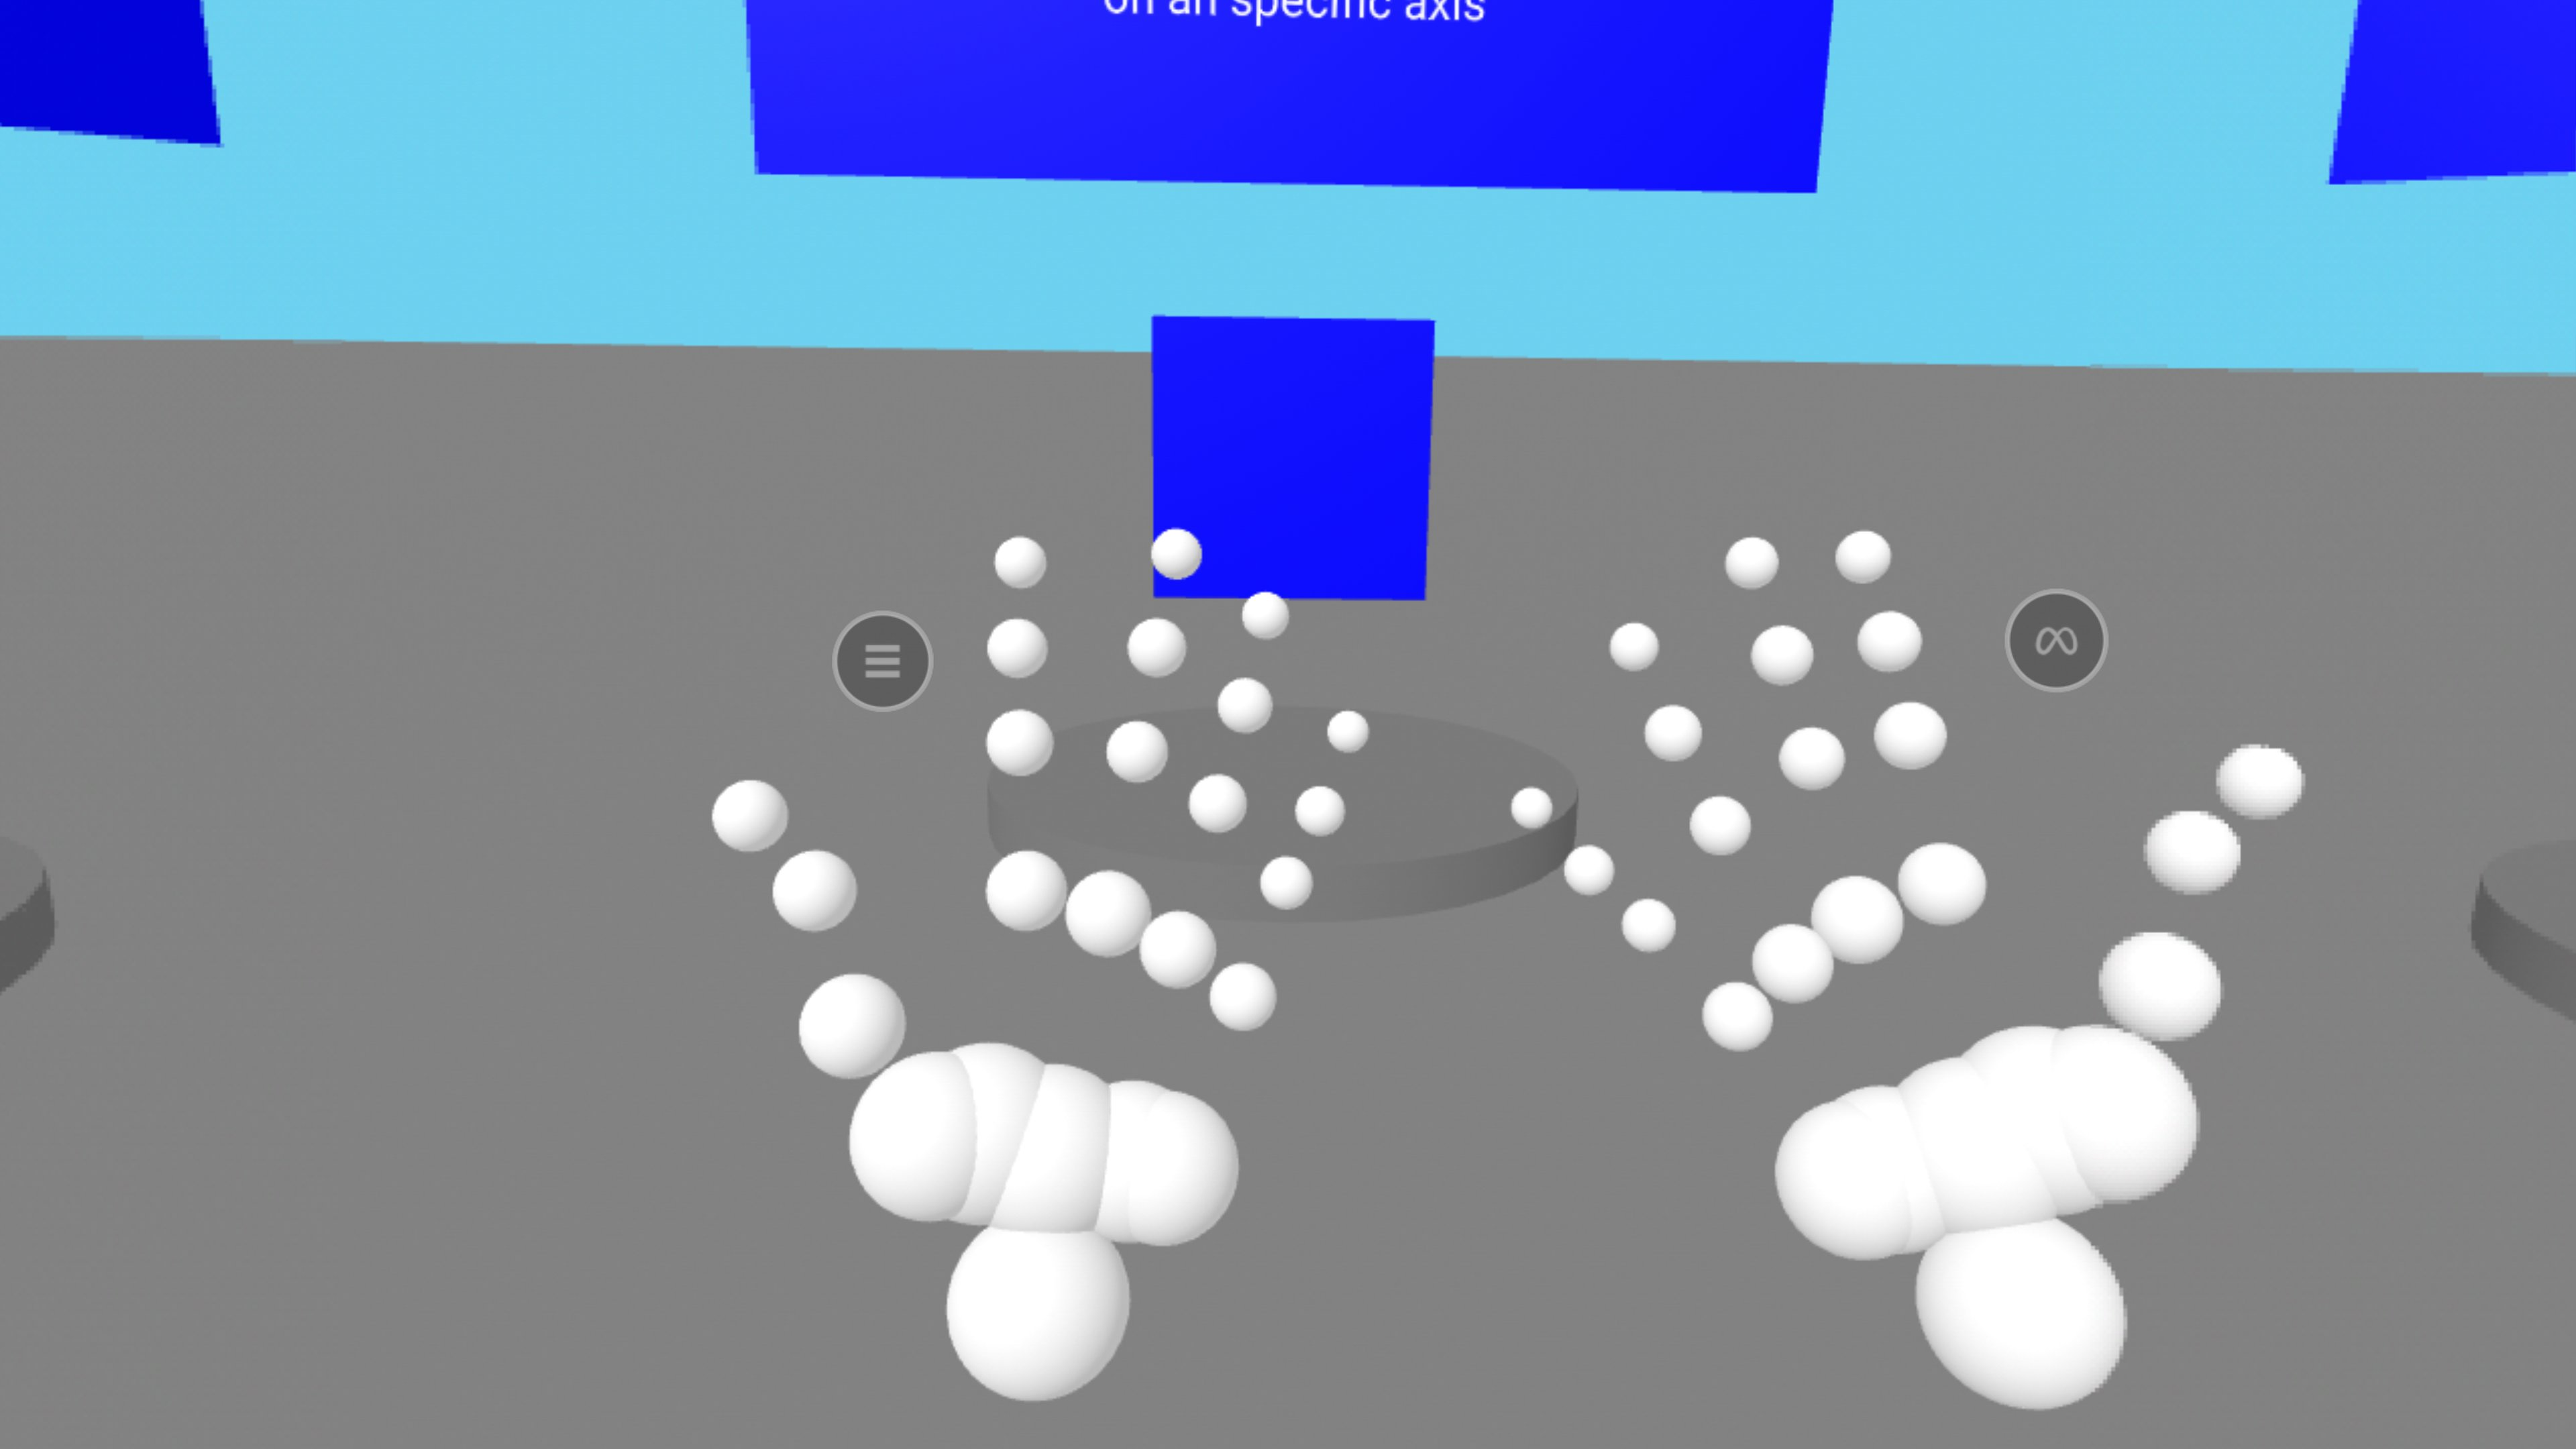
\includegraphics[width=0.7\textwidth]{img/manos.jpg} 
  % \fbox{\rule{0pt}{150pt} \rule{0.7\textwidth}{0pt}} 
  \caption{Manos en la escena}
  \label{fig:manos}
\end{figure}

Para poder renderizar la mano, era necesario definir todas las articulaciones que la componían, desde la muñeca hasta la punta de los dedos y todas las distintas falanges intermedias. Esto se debe a que, ya que se utilizo WebXR, al querer que el programa funcionase en navegadores, si no se definían las falanges, el programa no seria capaz de detectar aquellas que no fueron definidas.
En la figura \ref{fig:WebXR-manos} se muestra todas las articulaciones necesarias para que WebXR sea capaz de detectar y renderizar de forma correcta. 

Esto únicamente nos permite detectar las manos, pero no era suficiente para renderizarlas en la escena. Para ello era necesario crear una esfera por cada articulación. Utilizando el listado que posee todos los nombres de las articulaciones se crea una esfera por cada una y se guarda cada entidad en un diccionario, a cada entidad se le asignaba un nombre con el nombre de la articulación y la mano a la que pertenece, definido en el \texttt{schema} del componente.

Ya que estábamos utilizando WebXR, para poder acceder a la información de las posiciones de cada articulación era necesario acceder a la sesión XR y acceder a sus inputs, en este caso las manos. Esto se realizaba en una función llamada \texttt{updateSkeleton}. Por cada input de la sesión el programa accede al diccionario creado anteriormente y por cada articulación, a través de la sesión, se accede a su posición y tamaño y se actualiza la entidad correspondiente. También, en caso de que la articulación en cuestión sea la punta del dedo índice o la muñeca, se le añade un colisionador para 
poder interactuar con los elementos dentro de la escena. Esta actualización de la posición se realiza a cada frame, permitiendo un movimiento fluido y suave. En el fragmento de código \ref{lst:updateskeleton} se muestra el fragmento de la función mencionada, en él se muestra como se actualiza la posición de cada articulación: 

\begin{lstlisting}[caption=Actualización de las manos en la escena, captionpos=b, label=lst:updateskeleton]
  for (const [jointName, jointEntity] of Object.entries(this.joints)) {
    const joint = inputSource.hand.get(jointName);
    const jointPose = this.frame.getJointPose(joint, this.referenceSpace);
    const { x, y, z } = jointPose.transform.position;
    const radius = jointPose.radius || 0.008;  // Radio del joint
    jointEntity.setAttribute('position', { x, y, z });
    jointEntity.setAttribute('radius', radius);
    if (jointName == 'index-finger-tip' || jointName == 'wrist'){
        if (!jointEntity.hasAttribute('obb-collider')) {
          jointEntity.setAttribute('obb-collider', `size: ${radius * 2} ${radius * 2} ${radius * 2}`);
        }
    }
  }
\end{lstlisting}

Como se muestra en la figura \ref{lst:esferas} del capítulo \ref{chap:Desarrollo del proyecto}, al iniciar este componente se crea un diccionario el cual contiene todas las entidades que representan las articulaciones con sus respectivos nombres. En el fragmento que se acaba de mostrar se recorre dicho diccionario y utilizando la lógica explicada en la figura \ref{lst:defXR}, se accede a la información de la articulación en cuestión y se actualiza su entidad, además, en caso de que la articulación sea la punta del índice o la muñeca se comprueba si esta posee un colisionador y en caso de no tenerlo se le añade.

\subsection{Detección de gestos}
\label{subsec:deteccion-gestos}
Ahora que las manos se renderizan en la escena, era necesario detectar los gestos. Para ello, en una función nueva llamada \texttt{detectGesture}, al igual que la anterior, esta función se ejecutaba a cada frame. Se vuelve a acceder a la sesión de WebXR para obtener las posiciones de algunas articulaciones clave, como la muñeca, las puntas de los dedos y la falange intermedia del dedo índice.
Para el gesto \texttt{Pinch}, se utiliza la distancia entre la pinta del índice y del pulgar y si la distancia es lo suficiente pequeña o no se cambia una variable estado dentro del componente llamada \texttt{pinchState}, en esta variable booleana se almacena si se está realizando el gesto o no. Esta acción se ejecuta a través de una función dentro de la función \texttt{detectGesture}, y lo mismo ocurre con los gestos de \texttt{Openhand} y \texttt{Fist}, pese a que luego no se usan estos gestos. 

El caso del gesto de \texttt{Point} es diferente al de los otros gestos, la forma en la que se detecta es igual, pero los otros gestos al lanzar sus eventos correspondientes, estos son escuchados por los componentes interactivos directamente, mientras que para este gesto,
dentro de este mismo componente se realizan varios pasos previos. Este gesto está dividido en dos fases, cuando el usuario está haciendo la acción de \texttt{pistol} y cuando no. Cuando no, es cuando el usuario tiene el índice y el pulgar estirados, al realizar esta acción el programa crea un puntero en la punta del índice, esto se hace mediante la creación de una nueva entidad la cual se coloca en la punta del dedo índice y se le añade el atributo de \texttt{raycaster}, este puntero es el que posteriormente nos permite interactuar con los elementos a distancia. Cuando el usuario hace la acción de \texttt{pistol}, cuando el pulgar se pega al dedo índice, haciendo la acción de disparar con los dedos, se emite el evento de \texttt{clickStart} en el elemento que intersecciona con el puntero, es este evento el que posteriormente escuchara el componente correspondiente a esta acción. 

Para el puntero, era necesario que siguiera la dirección a la que apuntamos con la mano, para ello en una tercera función llamada \texttt{updatePointer} se volvía a acceder a la sesión XR y se tomaban las posiciones de la punta y nudillo del dedo índice y usando el vector que se generaba a partir de esas posiciones se actualizaba la dirección a la que apunta el vector.

\subsection{Componentes que interactual con la escena}
\label{subsec:componentes-interactivos}
\begin{itemize}
  \item Respecto a los componentes diseñados para interactuar con la escena, primero se creo el componente \textbf{\texttt{grabable}}, dicho componente es indispensable, ya que sin él los componentes que requieren interactuar físicamente con los elementos de la escena, como \texttt{drag} o \texttt{hoover}, no funcionarían en absoluto, para que funcionen correctamente, este componente es el encargado de escuchar los eventos de los colisionadores, al igual que comprueba el estado de la variable de \texttt{pinchState} del componente \texttt{manos}. Este componente no posee un \texttt{schema} y no es necesario definirlo dentro de la escena, en el HTML, ya que los otros componentes lo añaden directamente. Antes de realizar ninguna acción, este componente comprueba si la entidad a la que está ligado posee un colisionador y en caso de no tenerlo lo añade, esto es necesario, puesto que sin el colisionador tanto en la mano como en la otra entidad, no seriamos capaces de detectar las colisiones, posteriormente al escuchar los eventos, lo primero era diferenciar de qué mano provenían, para ello en caso de colisión se comprueba el nombre de la articulación que colisionó con el elemento de la escena y en el caso del gesto, como tenemos acceso a la información del componente \texttt{manos} y podemos distinguir entre la derecha y la izquierda, se copia en un par de constantes, una por mano, el valor de la variable \texttt{pinchState}. Dependiendo de la mano se actualiza una de las constantes de estado dentro de este componente, dichas constantes son: \texttt{this.colideRight}, \texttt{this.colideLeft}, \texttt{leftPinchState} y \texttt{rightPinchState}. También, independientemente de la mano, si se detecta una colisión,
se emite el evento de \texttt{hooverStart}, haciendo que la acción de \texttt{hoover} se realice, y ya dependiendo de las variables de estado que definen que mano está colisionando o haciendo el gesto se emiten los eventos para realizar las acciones de \texttt{drag}, \texttt{slide} o \texttt{stretch}, estos eventos luego son escuchados por los componentes correspondientes a cada acción.

  \item Para la acción de \textbf{\texttt{click}} es la única que no necesita pasar a través del componente \texttt{grabable} ya que no es necesario tocar el elemento con este componente para realizar esta acción. 
Al recibir los eventos correspondientes a la acción de start y end, este componente cambia el color del elemento o lo devuelve a la normalidad dependiendo de si el evento es el de start o el de end. 

  \item Para la acción de \textbf{\texttt{hoover}}, al recibir sus eventos, \texttt{hooverStart} o \texttt{hooverEnd}, el componente relacionado con esta acción hace que la entidad en la escena se vuelva ligeramente más trasparente en el caso del evento start y en el caso del evento end la devuelve a la normalidad. Esta acción nos permite saber de forma más visual cuando se es posible interaccionar con el elemento, ya que, como se mencionó previamente, la mayoría de componentes requieren que el usuario interactúe físicamente con los elementos para que los componentes funcionen.

  \item Respecto a la acción de \textbf{\texttt{slide}}, este componente es el único de los componentes que reaccionan con la escena que contiene un \texttt{schema}, en dicha sección el usuario puede definir por qué eje (X, Y o Z) o porque plano (XY, XZ o YZ) puede deslizarse el elemento en cuestión, en caso de no definir nada, por defecto se toma el eje X. Posteriormente, al recibir el evento correspondiente a la acción, se accede a la información compartida a través del evento, en dicha información se encuentra la posición del dedo índice de la mano izquierda, y dependiendo del eje o plano seleccionado en el \texttt{schema} de este componente, se puede deslizar el elemento a través de la escena en ese eje/plano que selecciono el usuario mientras los otros ejes se mantienen constantes.

  \item Para la acción de \textbf{\texttt{stretch}}, dentro de la información correspondiente al evento start de este gesto, se transmite la información de la punta del dedo índice de ambas manos. Como el funcionamiento de este componente es el de cambiar la escala del elemento que se esté agarrando, usando la información de ambos dedos, primero se calcula la distancia que hay entre ambos, la distancia inicial se guarda en una variable y a cada frame se calcula la distancia actual para guardarla en una segunda variable. Como se muestra en el fragmento de código \ref{lst:stretch}, usando ambas distancias se crea un factor de escalado para posteriormente multiplicar la escala actual del elemento por dicho factor, dicho factor se obtiene al dividir la escala actual que hay entre las dos manos entre la distancia inicial.
  \begin{lstlisting}[caption=Actualización del factor de escala, captionpos=b, label=lst:stretch]
  this.initialDistance = hand1Pos.distanceTo(hand2Pos);
  this.previousDistance = this.initialDistance;
  this.currentScale = this.el.object3D.scale.clone();

  tick: function () {  
    const hand1Pos = this.hand1.object3D.position;
    const hand2Pos = this.hand2.object3D.position;
    const currentDistance = hand1Pos.distanceTo(hand2Pos);
    if (Math.abs(currentDistance - this.previousDistance) > 0.01) {
    const scaleFactor = currentDistance / this.initialDistance;
    const newScale = this.currentScale.clone().multiplyScalar(scaleFactor);
    this.el.object3D.scale.copy(newScale);
    this.previousDistance = currentDistance;
    }
  }
\end{lstlisting}

  \item La acción de \textbf{\texttt{drag}} es la más compleja de todas. Para que funcionase correctamente esta acción se divide en dos fases, el reparenting y la rotación. Para que el elemento de la escena pudiera ser cogido con la mano, al escuchar los eventos correspondientes se realiza un reparenting, haciendo que la entidad sea hija de la punta del dedo índice en vez de ser hija de la escena como hasta ahora, la información de dicho dedo se transmite en los detalles del evento del mismo modo que se hacía en la acción de \texttt{Slide}. Realizar esta acción del reparenting nos permite arrastrar la entidad por la escena mientras el elemento y la articulación mantienen una distancia constante, esta misma acción se podría llegar a realizar haciendo cálculos de distancia entre el dedo y el centro de la entidad que deseamos mover y mantener dicha distancia e incluso el vector que las une, permitiendo que la entidad siga tanto los movimientos como la rotación de la nueva entidad padre, pero realizándolo de esta manera resulta más sencillo al no requerir ese tipo de cálculos. No obstante, por como se dibujan las articulaciones, únicamente se actualiza su posición y no la rotación haciendo que independientemente de la posición de la mano, las entidades que definen las articulaciones siempre estarán orientadas en la misma dirección, por tanto, es necesario un paso extra para la rotación.
Para ello primero se accede a la información de la mano, también transmitida en los detalles del evento, y se toma la posición de tres articulaciones, la punta y nudillo del dedo índice y el nudillo del dedo meñique. Con esas tres posiciones, se calculan los vectores que las unen y se crea un eje relativo ortonormal, el cual siempre imitara la rotación de la mano siendo el eje X el vector que une la punta y el nudillo del dedo índice, una vez con dicho eje, la entidad que estamos tomando copia dicho eje, esto hace que la entidad copie la rotación de la mano. En el siguiente fragmento de código se puede apreciar como se calcula el falso eje de coordenadas y como se aplica al objeto que se intenta desplazar.
\begin{lstlisting}[caption=Creación del falso eje de coordenadas, captionpos=b, label=lst:fake_coords]
  this.vectorX.copy(pos2).sub(pos1).normalize();  // Calcular el vector X (de esfera1 a esfera2)
  this.fakeX.copy(this.vectorX);

  this.vectorXZ.copy(pos3).sub(pos1);  // Calcular el vector Z (perpendicular al eje X, desde esfera3)
  this.vectorZ.crossVectors(this.vectorX, this.vectorXZ).normalize();
  this.fakeZ.copy(this.vectorZ);

  this.fakeY.crossVectors(this.fakeZ, this.fakeX).normalize();  // Calcular el eje Y como el producto cruzado entre X y Z
  
  if (this.fakeY.length() === 0) { // Asegurarnos de que el sistema sea ortonormal
    this.fakeZ.negate();
    this.fakeY.crossVectors(this.fakeZ, this.fakeX).normalize();
  }
  
  this.rotationMatrix.makeBasis(this.fakeX, this.fakeY, this.fakeZ);
  
  this.el.object3D.setRotationFromMatrix(this.rotationMatrix); 
\end{lstlisting}
\end{itemize}

En la figura \ref{fig:mosaico} se muestran algunas de las acciones explicadas en esta sección dentro de la escena.

\begin{figure}[H] 
  \centering
  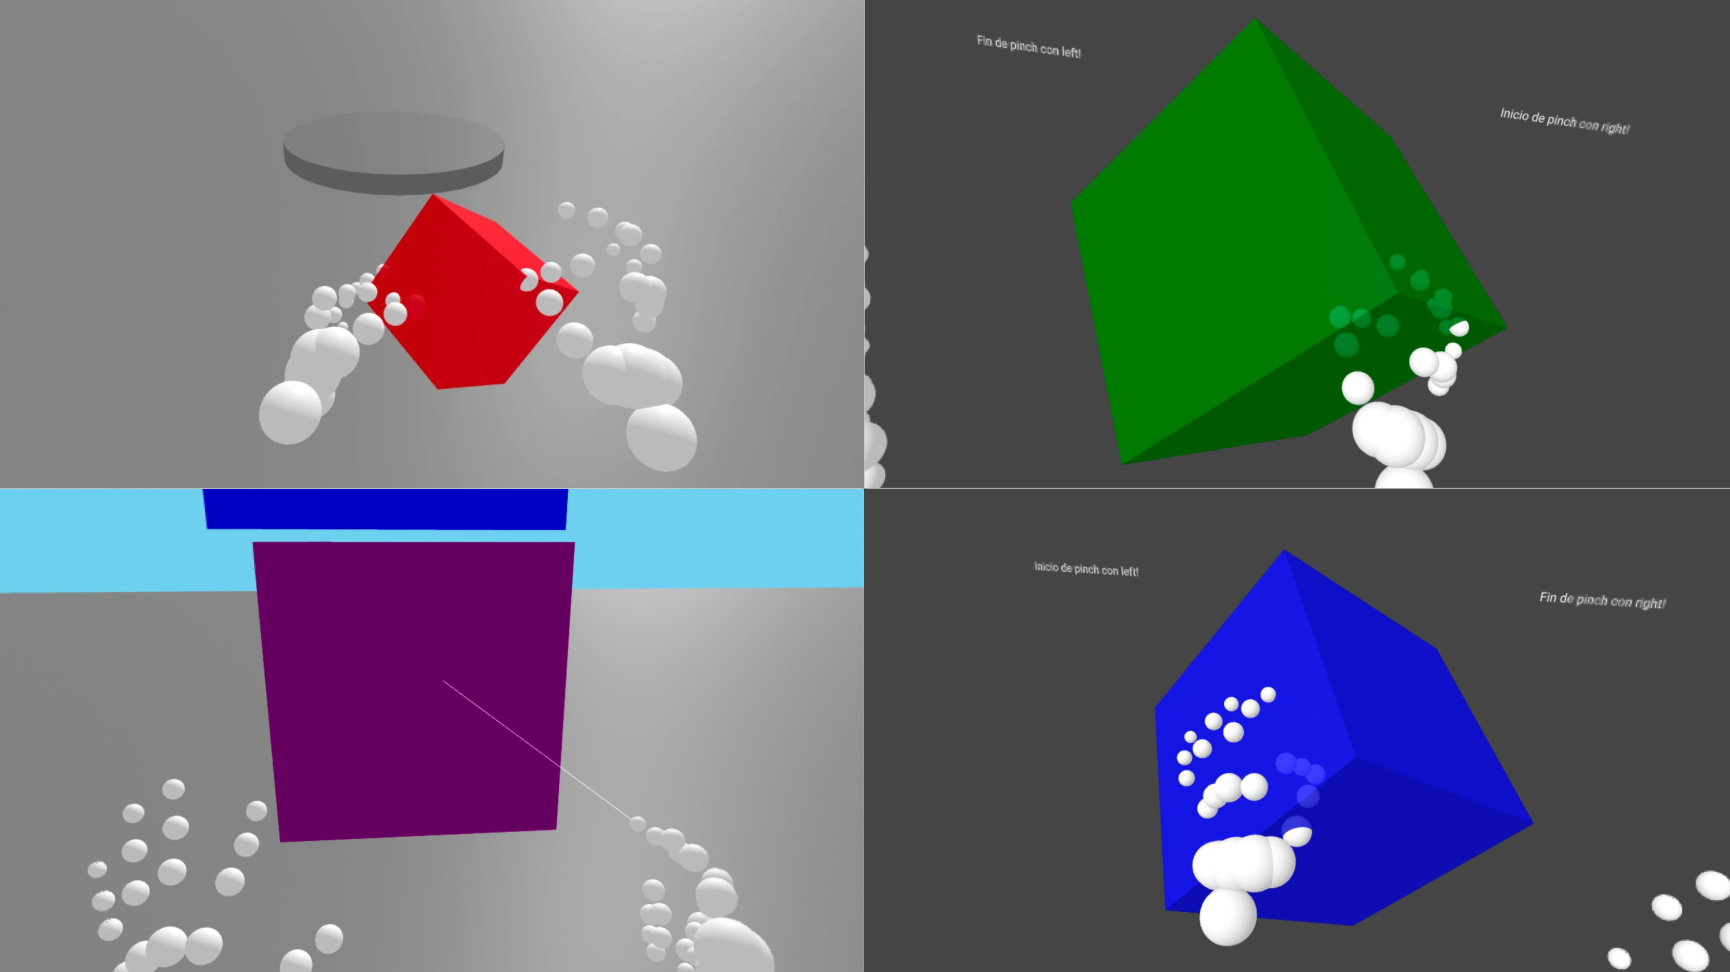
\includegraphics[width=0.7\textwidth]{img/colage.png} 
  % \fbox{\rule{0pt}{150pt} \rule{0.7\textwidth}{0pt}} 
  \caption{Acciones dentro de la escena}
  \label{fig:mosaico}
\end{figure}

\section{Construcción de escenas}
\label{sec:escenas}

Como ya se mencionó, este proyecto se planteó como una caja de herramientas para la creación de escenas o aplicaciones VR dentro un navegador. La capacidad de poder utilizar nuestras propias manos para poder interactuar con los distintos elementos que hay en la escena nos da posibilidades casi infinitas para utilizarlas. 

Algunos de los componentes se pueden utilizar directamente como los componentes de \texttt{drag}, \texttt{slide}, \texttt{stretch} o incluso \texttt{hoover}. Dado que la función de estos componentes es muy directa, estos se pueden aplicar directamente, estos componentes se pueden utilizar para toda clase de aplicaciones o escenas. Un ejemplo podría ser una aplicación de diseño de casas en VR,
donde el usuario a través de un meno selecciona los elementos que desee añadir (paredes, techos, muebles…) y utilizando los componentes creados en este proyecto podría mover, ajustar e incluso dimensionar los distintos elementos que él añada hasta obtener el resultado que desea, otra opción sería la creación de una aplicación de dibujo, donde el usuario pueda dibujar lo que desee. Un ejemplo de esto se puede encontrar en la demo de \textit{dibujar}\footnote{\url{https://github.com/JuJoarias/TFG/blob/main/demo/dibujar.html}} 

Respecto a la acción de \texttt{click}, ahora mismo está diseñada para cambiar el color del componente en el momento de click, pero de forma muy sencilla es posible cambiar esa lógica para que realice otras acciones. Esta acción puede ser muy útil para interactuar con distintos menús para el usuario o incluso en juegos que requieran disparar. Siguiendo la demo de \textit{juego click}\footnote{\url{https://github.com/JuJoarias/TFG/blob/main/demo/juego_click.html}} se puede encontrar el ejemplo descrito.

A continuación se muestra una versión simplificada de un archivo HTML, mostrando como se pueden utilizar los componentes creados durante este proyecto. En específico, el siguiente ejemplo corresponde a la escena de la demo dibujar.

\begin{lstlisting}[caption=Ejemplo de una escena, captionpos=b, label=lst:escena]
<html>
  <head>
    <meta charset="utf-8" />
    <title>Dibujar</title>
    <script src="https://aframe.io/releases/1.5.0/aframe.min.js"></script>
    <script> delete AFRAME.components["grabbable"]; </script>
    <script src="dibujar.js"></script>
  </head>
  <body>
    <a-scene 
      xr-mode-ui="enabled: true; enterVRDisabled: false;" 
      webxr="optionalFeatures: hand-tracking">
      <!-- Manos -->
      <a-entity>
        <a-camera></a-camera>
        <a-entity id="left-hand" manos="hand: left" ></a-entity>
        <a-entity id="right-hand" manos="hand: right" ></a-entity>
      </a-entity>
      <!-- Boligrafo -->
      <a-cylinder id="boligrafo" drag hoover></a-cylinder>
    </a-scene>
  </body>
</html>
\end{lstlisting}

%%%%%%%%%%%%%%%%%%%%%%%%%%%%%%%%%%%%%%%%%%%%%%%%%%%%%%%%%%%%%%%%%%%%%%%%%%%%%%%%
%%%%%%%%%%%%%%%%%%%%%%%%%%%%%%%%%%%%%%%%%%%%%%%%%%%%%%%%%%%%%%%%%%%%%%%%%%%%%%%%
% desarrollo del proyecto capitulo 4 %
%%%%%%%%%%%%%%%%%%%%%%%%%%%%%%%%%%%%%%%%%%%%%%%%%%%%%%%%%%%%%%%%%%%%%%%%%%%%%%%%

\cleardoublepage
\chapter{Desarrollo del proyecto}
\label{chap:Desarrollo del proyecto}
En este capítulo se describe de forma detallada como fue el desarrollo del proyecto. Dicho desarrollo
se describe en forma de sprints siguiendo una estructura de una metodología \textit{Agile}\cite{asana_agile_methodology}, pese a que el propio proyecto no siguió dicha metodología. 
El desarrollo explica desde los inicios y planteamiento del proyecto hasta obtener los resultados finales.

Por la forma en la que se fue planteando el proyecto, al final de cada sprint se planteaban los objetivos del siguiente para llegar al objetivo final de tener un seguimiento de manos funcional y que permitiese interactuar con los distintos elementos de la escena. 

\section{Sprint 0}
\label{sec:sprint0}
Puesta en marcha del proyecto, planteamiento con el tutor y dominio del uso básico de A-Frame.

\subsection{Objetivos}
\label{subsec:objetivo-principal0}
El objetivo principal de este sprint consiste en el dominio del uso básico de A-Frame. Aprender a usar de forma correcta como funcionan las escenas, al igual que la creación e implementación de componentes o el empleo de librerías de A-Frame.

\subsection{Tareas Realizadas}
\label{subsec:implementacion0}
La identificación de las necesidades y requisitos de un proyecto es una parte fundamental. Durante las primeras charlas con el tutor se plantearon algunos de los posibles objetivos a los que se podía llegar y los posibles caminos que puede tomar este proyecto. 
Al principio se plantearon varios caminos, pero la idea general de todos ellos era la creación de un sistema de seguimiento de manos que sea capaz de interactuar con distintos elementos dentro de la escena. 

Para lograr llegar a ese objetivo primero fue necesario dominar los elementos básicos de A-Frame como viene a ser la organización de la escena, el uso y creación de componentes y el uso de eventos. 
Para ello, primero se creo primero el repositorio de \textit{Git} con el que trabajaremos durante todo el proyecto. Para lograr el objetivo de este sprint, se realizaron una serie de escenas sencillas en las cuales se dominó el empleo y creación de componentes, al igual que el uso de eventos simples como el evento \texttt{click}.

\subsection{Resultados}
\label{subsec:resultados0}
Para familiarizarme aún más con el entorno de A-Frame se generaron una serie de escenas muy sencillas donde se generaba y utilizaba un componente customizado y se hacía uso del evento nativo de A-Frame \texttt{click}. Estas escenas permitieron un mayor entendimiento del funcionamiento tanto de componentes como de eventos, que fueron fundamentales para el resto del proyecto.
El resultado de dichas pruebas para mejorar la comprensión de A-Frame se pueden apreciar en la figura \ref{fig:sprint0}. En dicha escena, se crearon 2 componentes, el primero generaba un cubo y permite seleccionar los cubos de las paredes que lo forman, y el segundo crea una esfera animada que rebota dentro del cubo. 
\begin{figure}[H] 
  \centering
  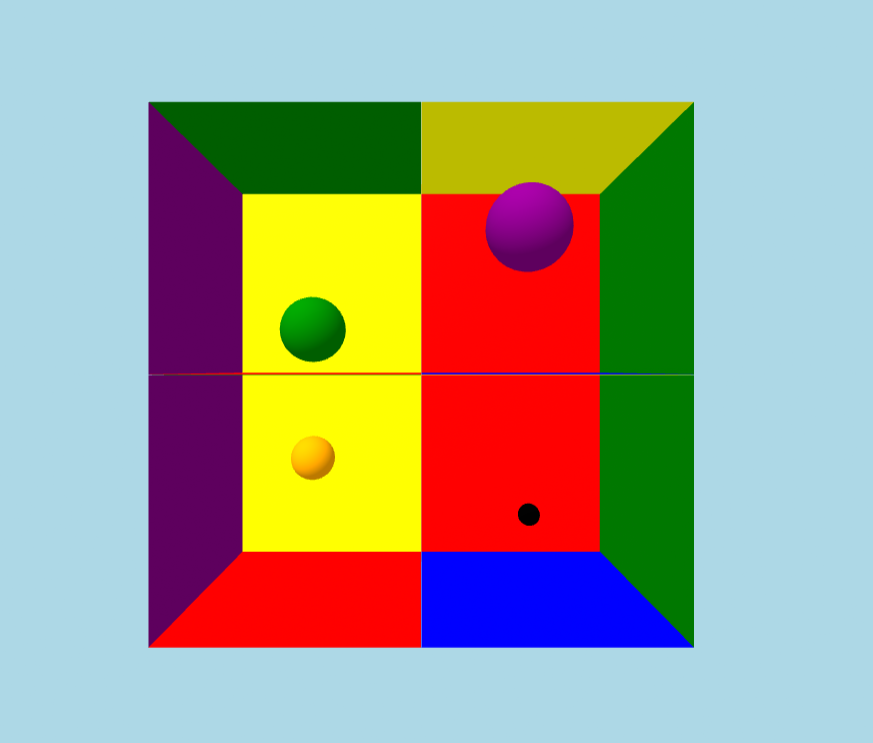
\includegraphics[width=0.7\textwidth]{img/primera_escena.png} 
  % \fbox{\rule{0pt}{150pt} \rule{0.7\textwidth}{0pt}} 
  \caption{Escena de test de A-Frame}
  \label{fig:sprint0}
\end{figure}

Tras la familiarización con el entorno de A-Frame y sus características, el proyecto fue formalizado formalmente. Tras ellos se planteo el siguiente sprint del proyecto, donde ya se empezarían los primeros pasos formales de este. 

\section{Sprint 1}
\label{sec:sprint1}
Investigación del handtracking y primeras implementaciones de este en el proyecto.

\subsection{Objetivos}
\label{subsec:objetivo-principal1}
El objetivo principal de este sprint era investigar y comprender el uso del handtracking en A-Frame. 
Además de obtener una primera demo del handtracking en la escena.

\subsection{Tareas Realizadas}
\label{subsec:implementacion1}
En este primer sprint oficial del proyecto, los primeros pasos fueron investigar el handtracking en A-Frame con los elementos ya existentes como \textit{\texttt{super hands}}\footnote{\url{https://github.com/c-frame/aframe-super-hands-component}}, o los componentes nativos de A-Frame \texttt{hand-controls} o \texttt{hand-tracking-controls}. Este era el paso principal en el que se basaría todo el proyecto, ya que sin una comprensión del funcionamiento del handtracking en A-Frame, este proyecto habría sido imposible de realizar.
Para ellos se usaron pequeñas escenas de prueba para comprender mejor el comportamiento de las manos en la realidad virtual, y del mismo modo, tener una idea más clara del objetivo final del aspecto de handtracking. 

Tras la investigación de las manos y puesto que el proyecto se desarrollo en A-Frame para que funcione en los navegadores, se decidió utilizar la tecnología de WebXR para el seguimiento de manos, puesto que esta tecnología ya posee un sistema preparado para ello. Además, usando la tecnología de WebXR nos permitía trabajar con cada una de las articulaciones de la mano de forma independiente, permitiéndonos tomar la información necesaria de las articulaciones cuando es necesario. 

Siguiendo la documentación de \textit{WebXR}\footnote{\url{https://www.w3.org/TR/webxr-hand-input-1/}}, se empezó el desarrollo de las manos. Para ello, en el código fue necesario tratar cada una de las manos de forma independiente, del mismo modo que cada una de las articulaciones, como se muestra en el esquema de las manos de WebXR en la figura \ref{fig:WebXR-manos}. 

\begin{figure}[H] 
  \centering
  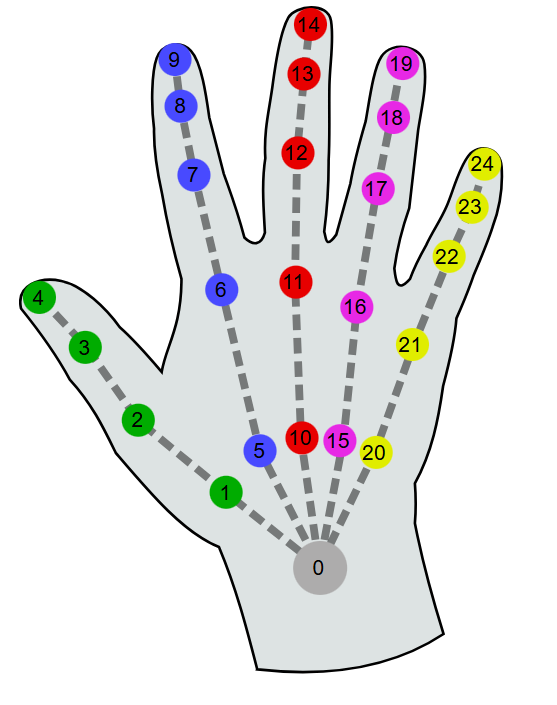
\includegraphics[width=0.4\textwidth]{img/webxr-mano.png} 
  \caption{Esquema manos segun WebXR}
  \label{fig:WebXR-manos}
\end{figure}

Para poder crear las manos de forma exitosa dentro del entorno de realidad virtual siguiendo WebXR, primero se crea el componente que será el encargado de detectar y dibujar las manos en este proyecto, dicho componente se llama \texttt{hand-skeleton}. Dicho componente no tenía un \texttt{schema}, en el \texttt{init} se definían las distintas variables que eran necesarias para el funcionamiento del código. 
En el HTML que define la escena únicamente era necesario añadir una vez el componente como una entidad. Pero como el componente trabaja directamente con la API de WebXR, era imprescindible definir todas y cada una de las articulaciones, como se muestra en el fragmento de código \ref{lst:articulaciones}, pero esa definición únicamente se realizaba en el código de JavaScript.
\begin{lstlisting}[caption=Definición de articulaciones, captionpos=b, label=lst:articulaciones]
  const orderedJoints = [
    ["wrist"],
    ["thumb-metacarpal", "thumb-phalanx-proximal", "thumb-phalanx-distal", "thumb-tip"],
    ...
    ["pinky-finger-metacarpal", "pinky-finger-phalanx-proximal", "pinky-finger-phalanx-intermediate", "pinky-finger-phalanx-distal", "pinky-finger-tip"]
  ];
\end{lstlisting}
Después de definir todas las articulaciones era necesario procesarlas. 
Para ello, se creo la función que se muestra en el fragmento de código \ref{lst:manos-codigo}. En la función \texttt{renderHandSkeleton} se crea un bucle de código el cual, toma la sesión XR de la escena y por cada input de la sesión, toma cada una de las articulaciones, las detecta en la mano y genere una esfera en una segunda función únicamente encargada de generar esferas. Dichas esferas se crean en la posición correspondiente a la mano real
y también se ajusta el radio de la esfera para que coincida con la mano, esta función nos permite renderizar en la escena las manos del usuario de forma que parezca lo más natural posible. 

\begin{lstlisting}[caption=Dibujo de las manos en la escena, captionpos=b, label=lst:manos-codigo]
  renderHandSkeleton: function () {
    const session = this.el.sceneEl.renderer.xr.getSession();
    if (!session || !this.frame || !this.referenceSpace) {
        return;
    }
    const inputSources = session.inputSources;
    for (const inputSource of inputSources) {
      if (inputSource.hand) {
        const hand = inputSource.hand;
        const handedness = inputSource.handedness; // Determina si es la mano derecha o izquierda
        for (const finger of orderedJoints) {
          for (const jointName of finger) {
            const joint = hand.get(jointName);
            if (joint) {
              const jointPose = this.frame.getJointPose(joint, this.referenceSpace);
              if (jointPose) {
                const position = jointPose.transform.position;
                if (!this.spheres[handedness + '_' + jointName]) {
                  this.spheres[handedness + '_' + jointName] = this.drawSphere(jointPose.radius, position);
                } else {
                  this.spheres[handedness + '_' + jointName].object3D.position.set(position.x, position.y, position.z);
                }
              }
            }
          }
        }
      }
    }
  },
\end{lstlisting}

Esta función se encuentra dentro de la función \texttt{tick} del componente manos, así que a cada frame el propio código revisa la posición de todas y cada una de las articulaciones para cada una 
de las dos manos de entrada.
Además de detectar y dibujar las manos en la escena, en esta primera demo se implementó el gesto de \texttt{Pinch}, distinguiendo cada mano y realizando una acción distinta dependiendo de la mano que lo realizase. 

Primero, para la detección del gesto se creo la función de \texttt{detectGestures}, como se muestra en el fragmento de código \ref{lst:firstdetectGesture}. En dicha función, se tomaba la posición de la punta del dedo índice y del pulgar y se calculaba la distancia entre ambos puntos.

\begin{lstlisting}[caption=Función detectGestures, captionpos=b, label=lst:firstdetectGesture]
  detectGestures: function () {
    const session = this.el.sceneEl.renderer.xr.getSession();
    const inputSources = session.inputSources;
    let rightPinching = false;
    let leftPinching = false;
    for (const inputSource of inputSources) {
      if (inputSource.hand) {
        const thumbTip = this.frame.getJointPose(inputSource.hand.get("thumb-tip"), this.referenceSpace);
        const indexTip = this.frame.getJointPose(inputSource.hand.get("index-finger-tip"), this.referenceSpace);
        if (thumbTip && indexTip) {
          const distance = calculateDistance(thumbTip.transform.position, indexTip.transform.position);
          if (distance < pinchDistance) {
            if (inputSource.handedness === 'right') {
              rightPinching = true;
              if (!this.rightPinching) {
                this.createBoxAtHand(inputSource.hand);  
              }
            } else if (inputSource.handedness === 'left') {
              leftPinching = true;
              if (!this.leftPinching) {
                this.selectObjectAtHand(inputSource.hand); // Selecciona un objeto cercano para mover
              }
            }
          }
        }
      }
    }
    this.rightPinching = rightPinching;
    this.leftPinching = leftPinching;
  },
\end{lstlisting}

Si la distancia era inferior a 0.02 (valor obtenido tras realizar varias pruebas), se comprobaba que mano era la que lo realizaba y luego se llamaba a la función correspondiente. 
Si se trataba de la mano derecha, se creaba un cubo verde en la posición de la punta del dedo índice. Y si se trataba de la mano izquierda, si esta se encontraba lo bastante cerda de uno de los cubos creados por la mano derecha (a una distancia inferior a 0.15) la posición del cubo copiaría la de la punta del dedo índice izquierdo hasta que se soltase el gesto.

\subsection{Resultados}
\label{subsec:resultados1}

Como resultado de este sprint se creo la demo de \textit{pinch test}\footnote{\url{https://github.com/JuJoarias/TFG/blob/main/first_steps/first_hands/pinch_test.html}}, en la figura \ref{fig:sprint1} se aprecian los resultados de este sprint.

\begin{figure}[H] 
  \centering
  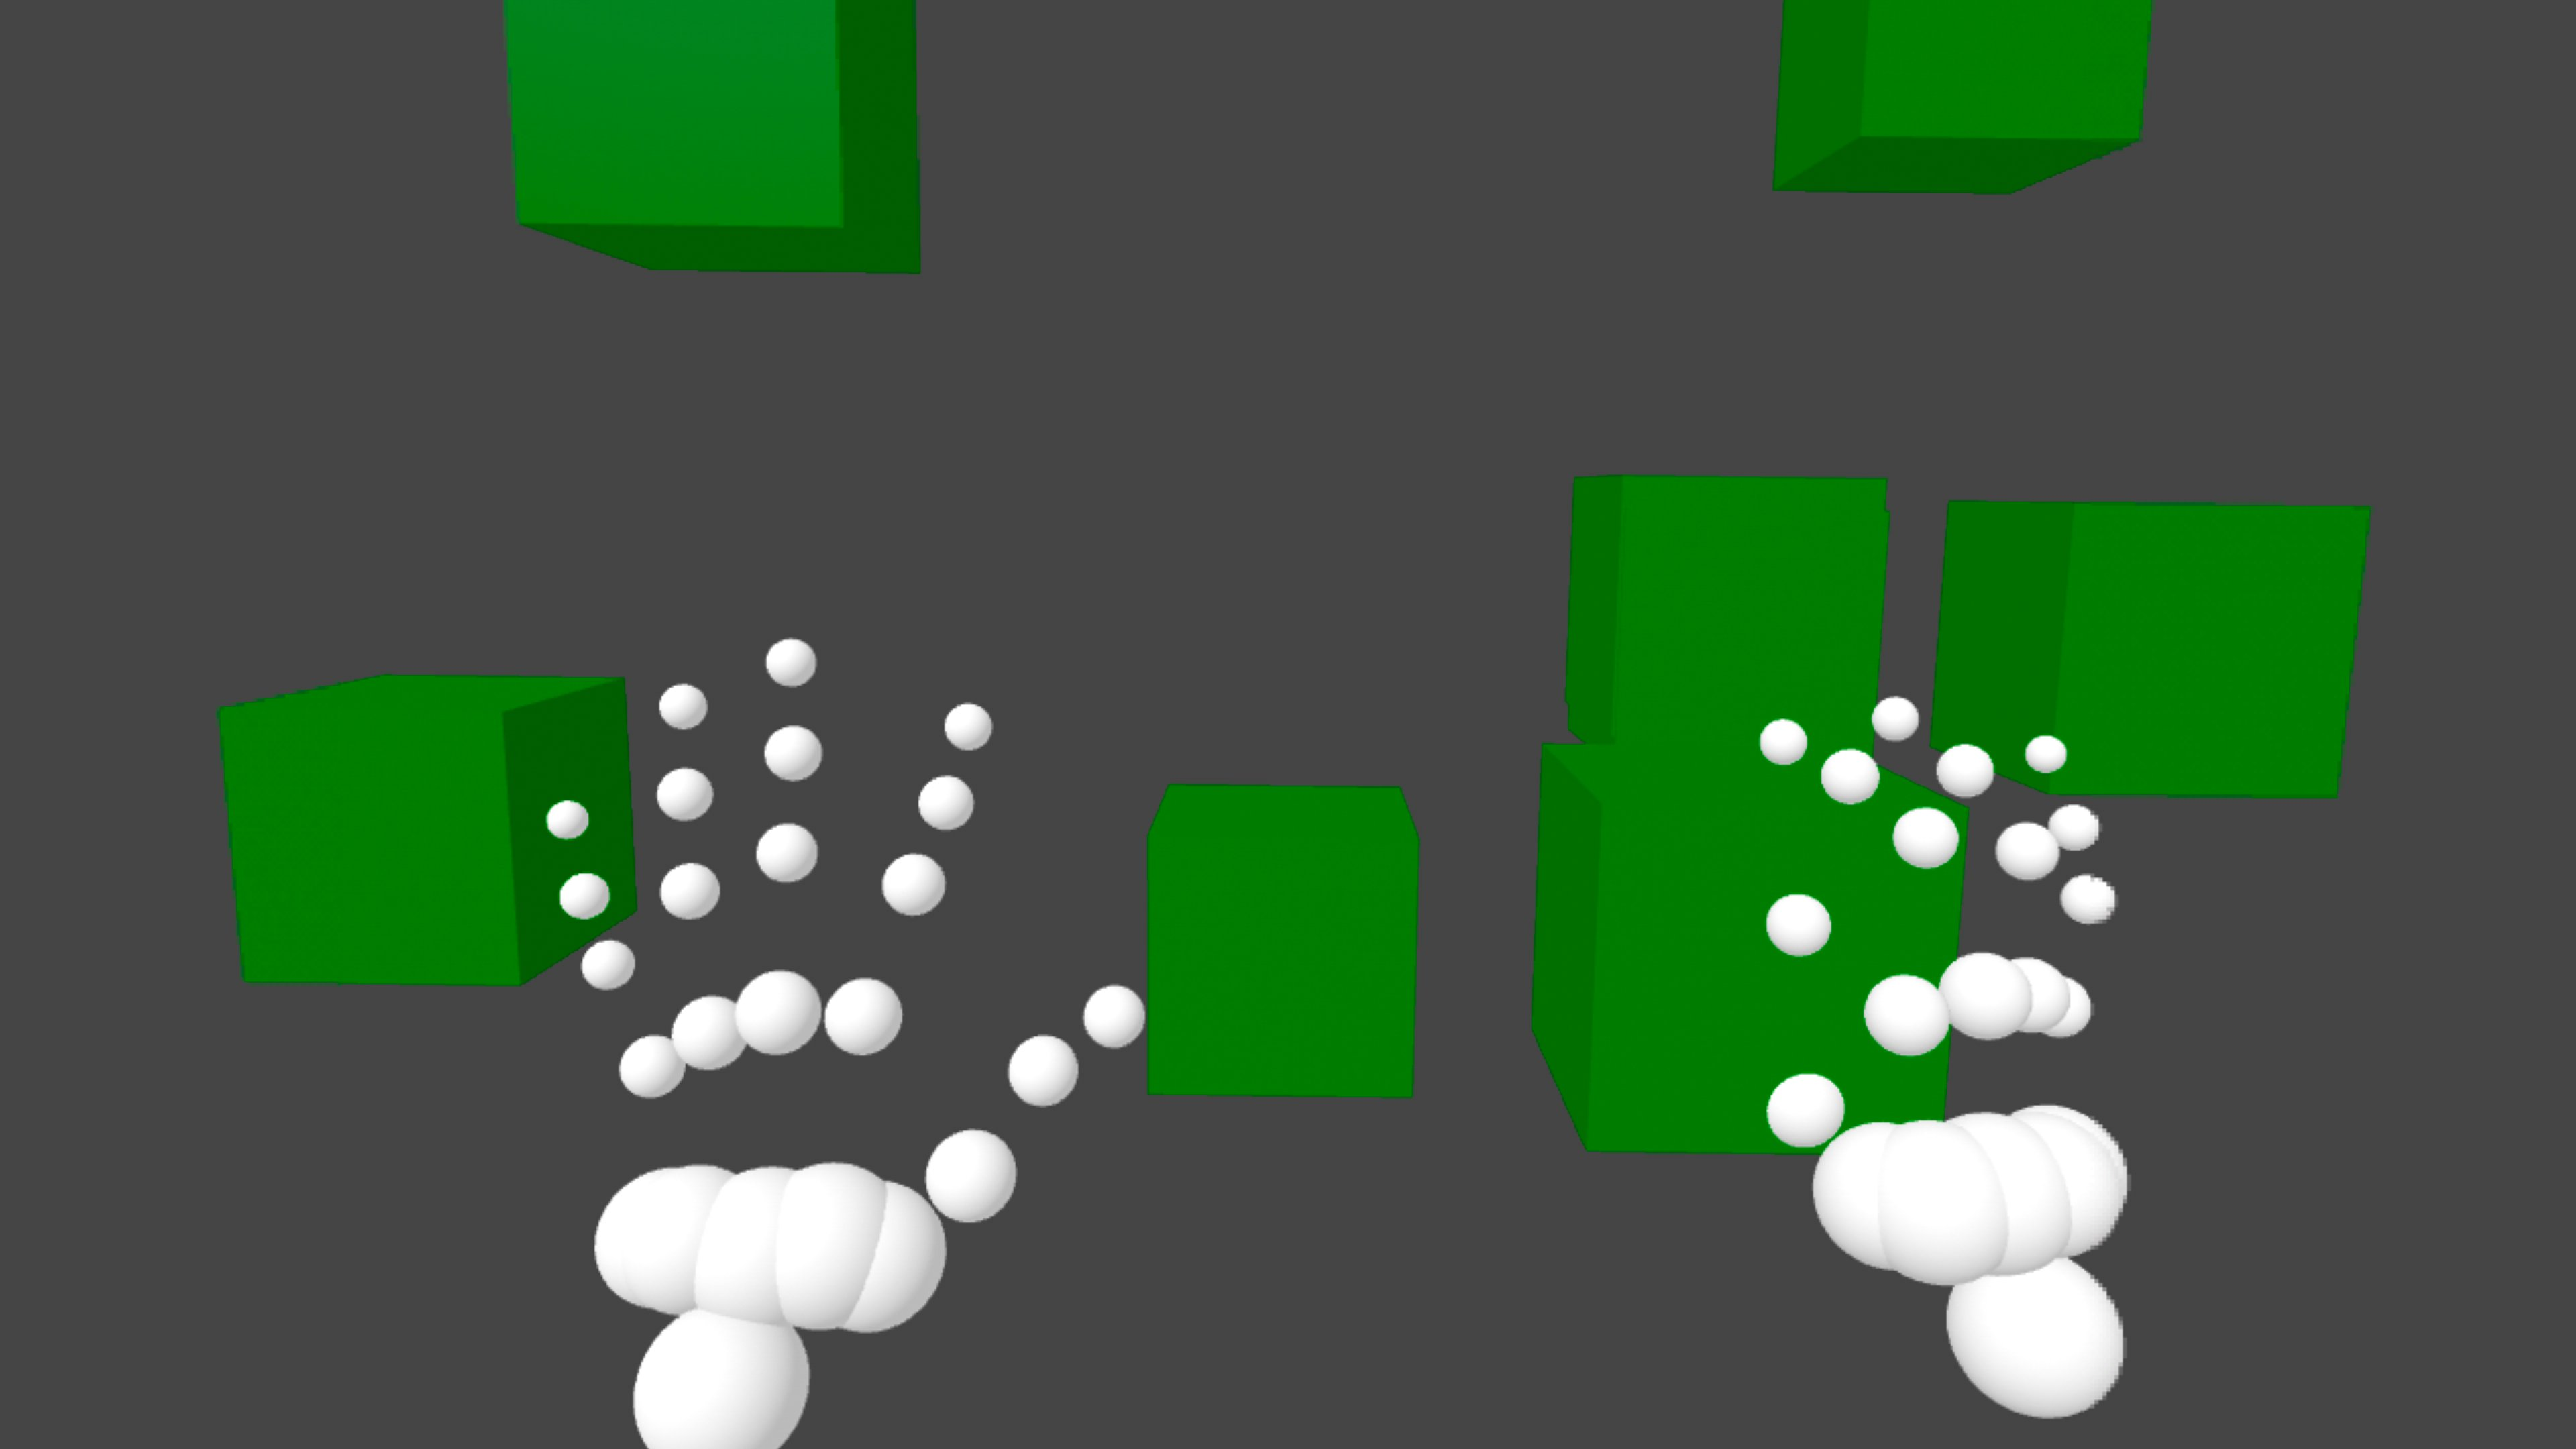
\includegraphics[width=0.7\textwidth]{img/primeras_manos.jpg} 
  % \fbox{\rule{0pt}{150pt} \rule{0.7\textwidth}{0pt}} 
  \caption{Primera demo de manos}
  \label{fig:sprint1}
\end{figure}

Las esferas se dibujaban correctamente y los gestos funcionaban, pero había bastantes aspectos a mejorar. Primero, por sugerencia del tutor,
se debía modificar el componente para que fuese necesario añadirlo 2 veces a la escena, 1 por cada mano. También, respecto al gesto, con la mano derecha había que cambiar el funcionamiento
ya que el que creara un cubo no seria necesario más adelante. Y respecto a la mano izquierda, se identificó que a la hora de tomar el cubo, este se transportaba hacia la posición del dedo índice. 
Y aunque esto era lo deseado de primeras, visualmente no quedaba bien por el hecho de que si se agarraba una esquina el cubo se transportaba, tragándose la mano en vez de agarrar el cubo mientras mantenía la distancia entre el dedo y el centro del cubo. 
Aparte de eso, en el caso de que hubiese más de un cubo muy pegado, el código no identificaba siempre de forma correcta el más cercano, haciendo que a veces se tomara el cubo no deseado.

Todos estos factores dieron paso al siguiente sprint, donde se corregirían los errores resaltados. Aparte se intentaría optimizar la creación de las manos y se añadiría la emisión y gestión de eventos, ya que en esta primera demo, al realizar el gesto, se llama a la función correspondiente si utilizar eventos. 

\section{Sprint 2}
\label{sec:sprint2}
Introducción de eventos al sistema y optimización del manejo de manos. 

\subsection{Objetivos}
\label{subsec:objetivo-principal2}
Los objetivos de este sprint consistían en el replanteamiento de la detección de gestos, además de la optimización de la forma de renderización de las manos en la escena y la detección de los gestos con el fin de obtener un código más optimizado. 

\subsection{Tareas Realizadas}
\label{subsec:implementacion2}
Primero, se reorganizo el componente encargado de dibujar las manos que se creo en el sprint anterior. Dicho componente se renombro a \texttt{manos}, nombre que se mantendría hasta el final del proyecto. A dicho componente se le añadió un \texttt{schema}. 
En dicho \texttt{schema} hay únicamente una variable llamada \texttt{hand}, dicha variable únicamente acepta \texttt{left} o \texttt{right} como entradas. Este cambio era para que el componente distinguiera las manos y únicamente dibujase una mano a la vez, esto hizo que para dibujar ambas manos en la escena fuese necesario añadir el componente 2 veces, 1 por cada mano. 
También, se modifico la función \texttt{init}. Ahora, aparte de definir los valores iniciales de las variables utilizadas, realiza un bucle que recorre la constante que contiene todas las articulaciones y por cada una crea una esfera. Dichas esferas son añadidas a la escena y también se crea un diccionario al que se le añade el nombre y entidad de cada articulación.
Este bucle se puede apreciar en el fragmento de código \ref{lst:esferas}. Como se puede apreciar, esto no nos permite detectar las manos y utilizarlas en la escena, simplemente prepara las entidades que representaran la mano dentro de la escena.

\begin{lstlisting}[caption=Creación de las esferas de las articulaciones, captionpos=b, label=lst:esferas]
  orderedJoints.flat().forEach((jointName) => {
    const jointEntity = document.createElement('a-sphere');
    jointEntity.setAttribute('color', 'white'); 
    this.el.appendChild(jointEntity);
    this.joints[jointName] = jointEntity;
  });
\end{lstlisting}

Para la actualización de la posición de todas las articulaciones se creó la función que se muestra en el fragmento de código \ref{lst:nuevas_manos}. Esa nueva función es una versión actualizada de la que se creo en el sprint anterior. 
La principal diferencia con el código previo es que este únicamente trabaja con la mano que se definió en el \texttt{schema} y trabaja directamente con las entidades que están guardadas en el diccionario que se creo en el \texttt{init}. 

\begin{lstlisting}[caption=Actualización de las manos, captionpos=b, label=lst:nuevas_manos]
  updateSkeleton: function () {
    const session = this.el.sceneEl.renderer.xr.getSession();
    const inputSources = session.inputSources;
    for (const inputSource of inputSources) {
      if (inputSource.handedness === this.data.hand && inputSource.hand) {
        for (const [jointName, jointEntity] of Object.entries(this.joints)) {
          const joint = inputSource.hand.get(jointName);
          const jointPose = this.frame.getJointPose(joint, this.referenceSpace);
          
          if (jointPose) {
            const { x, y, z } = jointPose.transform.position;
            const radius = jointPose.radius; 
            jointEntity.setAttribute('position', { x, y, z });
            jointEntity.setAttribute('radius', radius || 0.008);
          } else {
            jointEntity.setAttribute('position', '0 0 0'); // Esconder si no hay datos
          }
        }
      }
    }
  },
\end{lstlisting}

Para la detección del gesto la lógica general permanece igual, pero en vez de llamar a otras funciones se emiten los eventos \texttt{pinchstart} y \texttt{pinchend} dependiendo de si se está realizando el gesto o no y junto al evento se envía como argumento de este la mano que lo realiza, la derecha u izquierda.

Para escuchar los eventos, se creo el componente \texttt{detector}. Este componente posee 2 variables en su \texttt{schema}. La primera es que mano detectara, del mismo modo que el componente \texttt{manos}, y la segunda es un target. El target es principalmente para debug de la escena, ya que para esta demo se añadieron 2 entidades a la escena, las cuales 
eran texto. Así que el target seria el ID de una de esas entidades de texto.
Este componente cada vez que recibiese un evento se encargaría de modificar el texto del target, señalando si se ha iniciado o terminado el gesto y de que mano. 

\subsection{Resultados}
\label{subsec:resultados2}
El resultado de este sprint fue el código \textit{componentes}\footnote{\url{https://github.com/JuJoarias/TFG/blob/main/first_steps/first_hands/componentes.html}}.

\begin{figure}[H] 
  \centering
  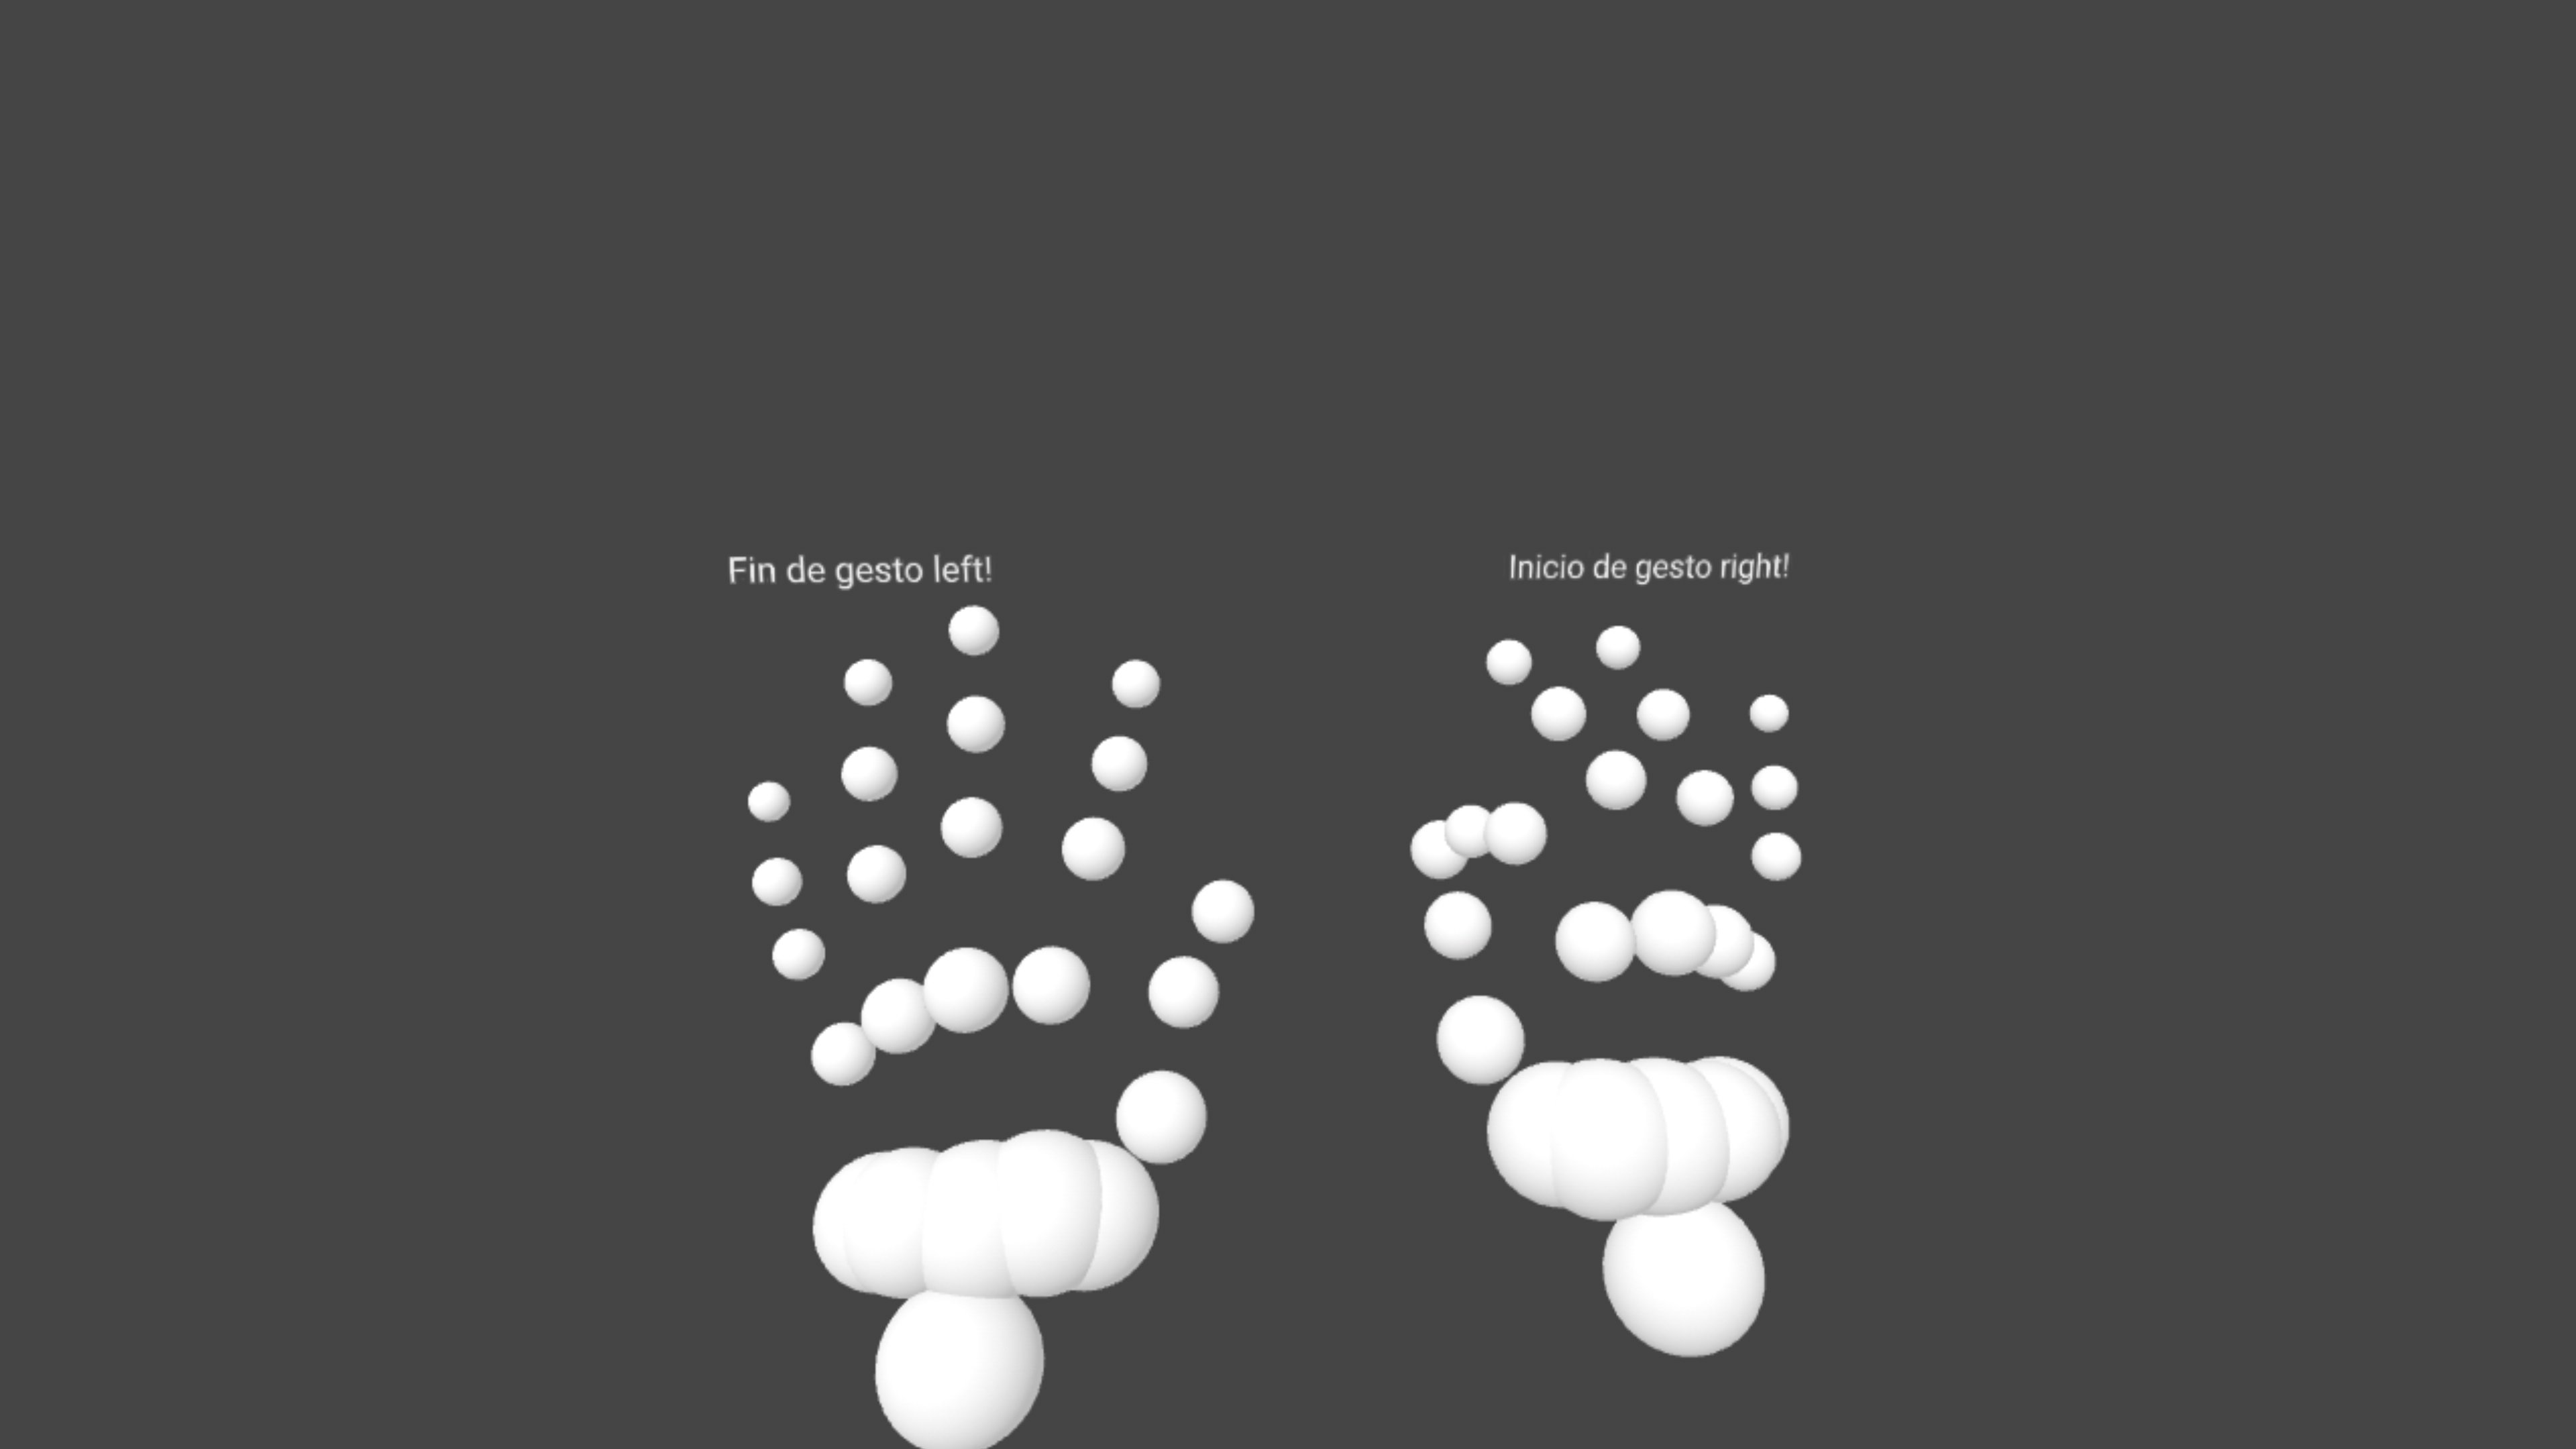
\includegraphics[width=0.7\textwidth]{img/primer_gesto.jpg}
  % \fbox{\rule{0pt}{150pt} \rule{0.7\textwidth}{0pt}} 
  \caption{Primer gesto}
  \label{fig:sprint2}
\end{figure}

En este sprint a nivel visual en la escena no había grandes cambios ya que el objetivo principal era la optimización de la creación de las manos y la introducción de los eventos. 
Como se aprecia en la figura \ref{fig:sprint2}, dentro de la escena se dibujan las manos correctamente y los textos se modifican como es debido. Para esta demo, para los gestos únicamente se implemento el cambio de texto ya que 
como aún no se trabajaba con los gestos y hacía falta añadir más, se quería una forma más sencilla de comprobar que los eventos se emitían y escuchaban correctamente. 

\section{Sprint 3}
\label{sec:sprint3}
Introducción de nuevos gestos de las manos a la escena.

\subsection{Objetivos}
\label{subsec:objetivo-principal3}
El objetivo principal de este sprint era el introducir la lógica de los gestos \texttt{Fist}, \texttt{Point} y \texttt{Openhand} ya que hasta ahora únicamente se había implementado el gesto \texttt{Pinch}.

\subsection{Tareas Realizadas}
\label{subsec:implementacion3}
Para conseguir implementar los nuevos gestos principalmente hizo falta modificar la función de \texttt{detectGesture}, aparte de eso, para poder distinguir bien que gesto se está realizando, en el \texttt{init} se definió una variable booleana por cada gesto, las cuales cambian dependiendo de si se está realizando el gesto o no. Estas variables se implementaron ya que, como la comprobación de los gestos y emisión de estos se realizan en la función \texttt{tick}, si no se implementa esta lógica, se emitiría el mismo evento repetidas veces cuando únicamente es necesaria una vez.

Para ello, primero se buscaba la posición de la punta de todos los dedos y de la muñeca. Una vez con todas las posiciones obtenidas, mediante una función se calculaba la distancia de la punta del dedo correspondiente a la muñeca y si esa distancia era inferior a 0.09 (obtenido luego de varias pruebas para que sea una distancia óptima), se definía que el dedo en cuestión estaba doblado.
Para cada dedo hay una constante booleana que este True si el dedo está doblado y false si está estirado. Ahora con la información de cada dedo se comprueba si están estirados o no y dependiendo del estado de los dedos y de si la variable de estado de los gestos está a True o False, se emite el evento start o end correspondiente a cada gesto. 

\subsection{Resultados}
\label{subsec:resultados3}
Como resultado, se obtuvo la demo de \textit{nuevos gestos}\footnote{\url{https://github.com/JuJoarias/TFG/blob/main/first_steps/second_hands/nuevos_gestos.html}}

\begin{figure}[H] 
  \centering
  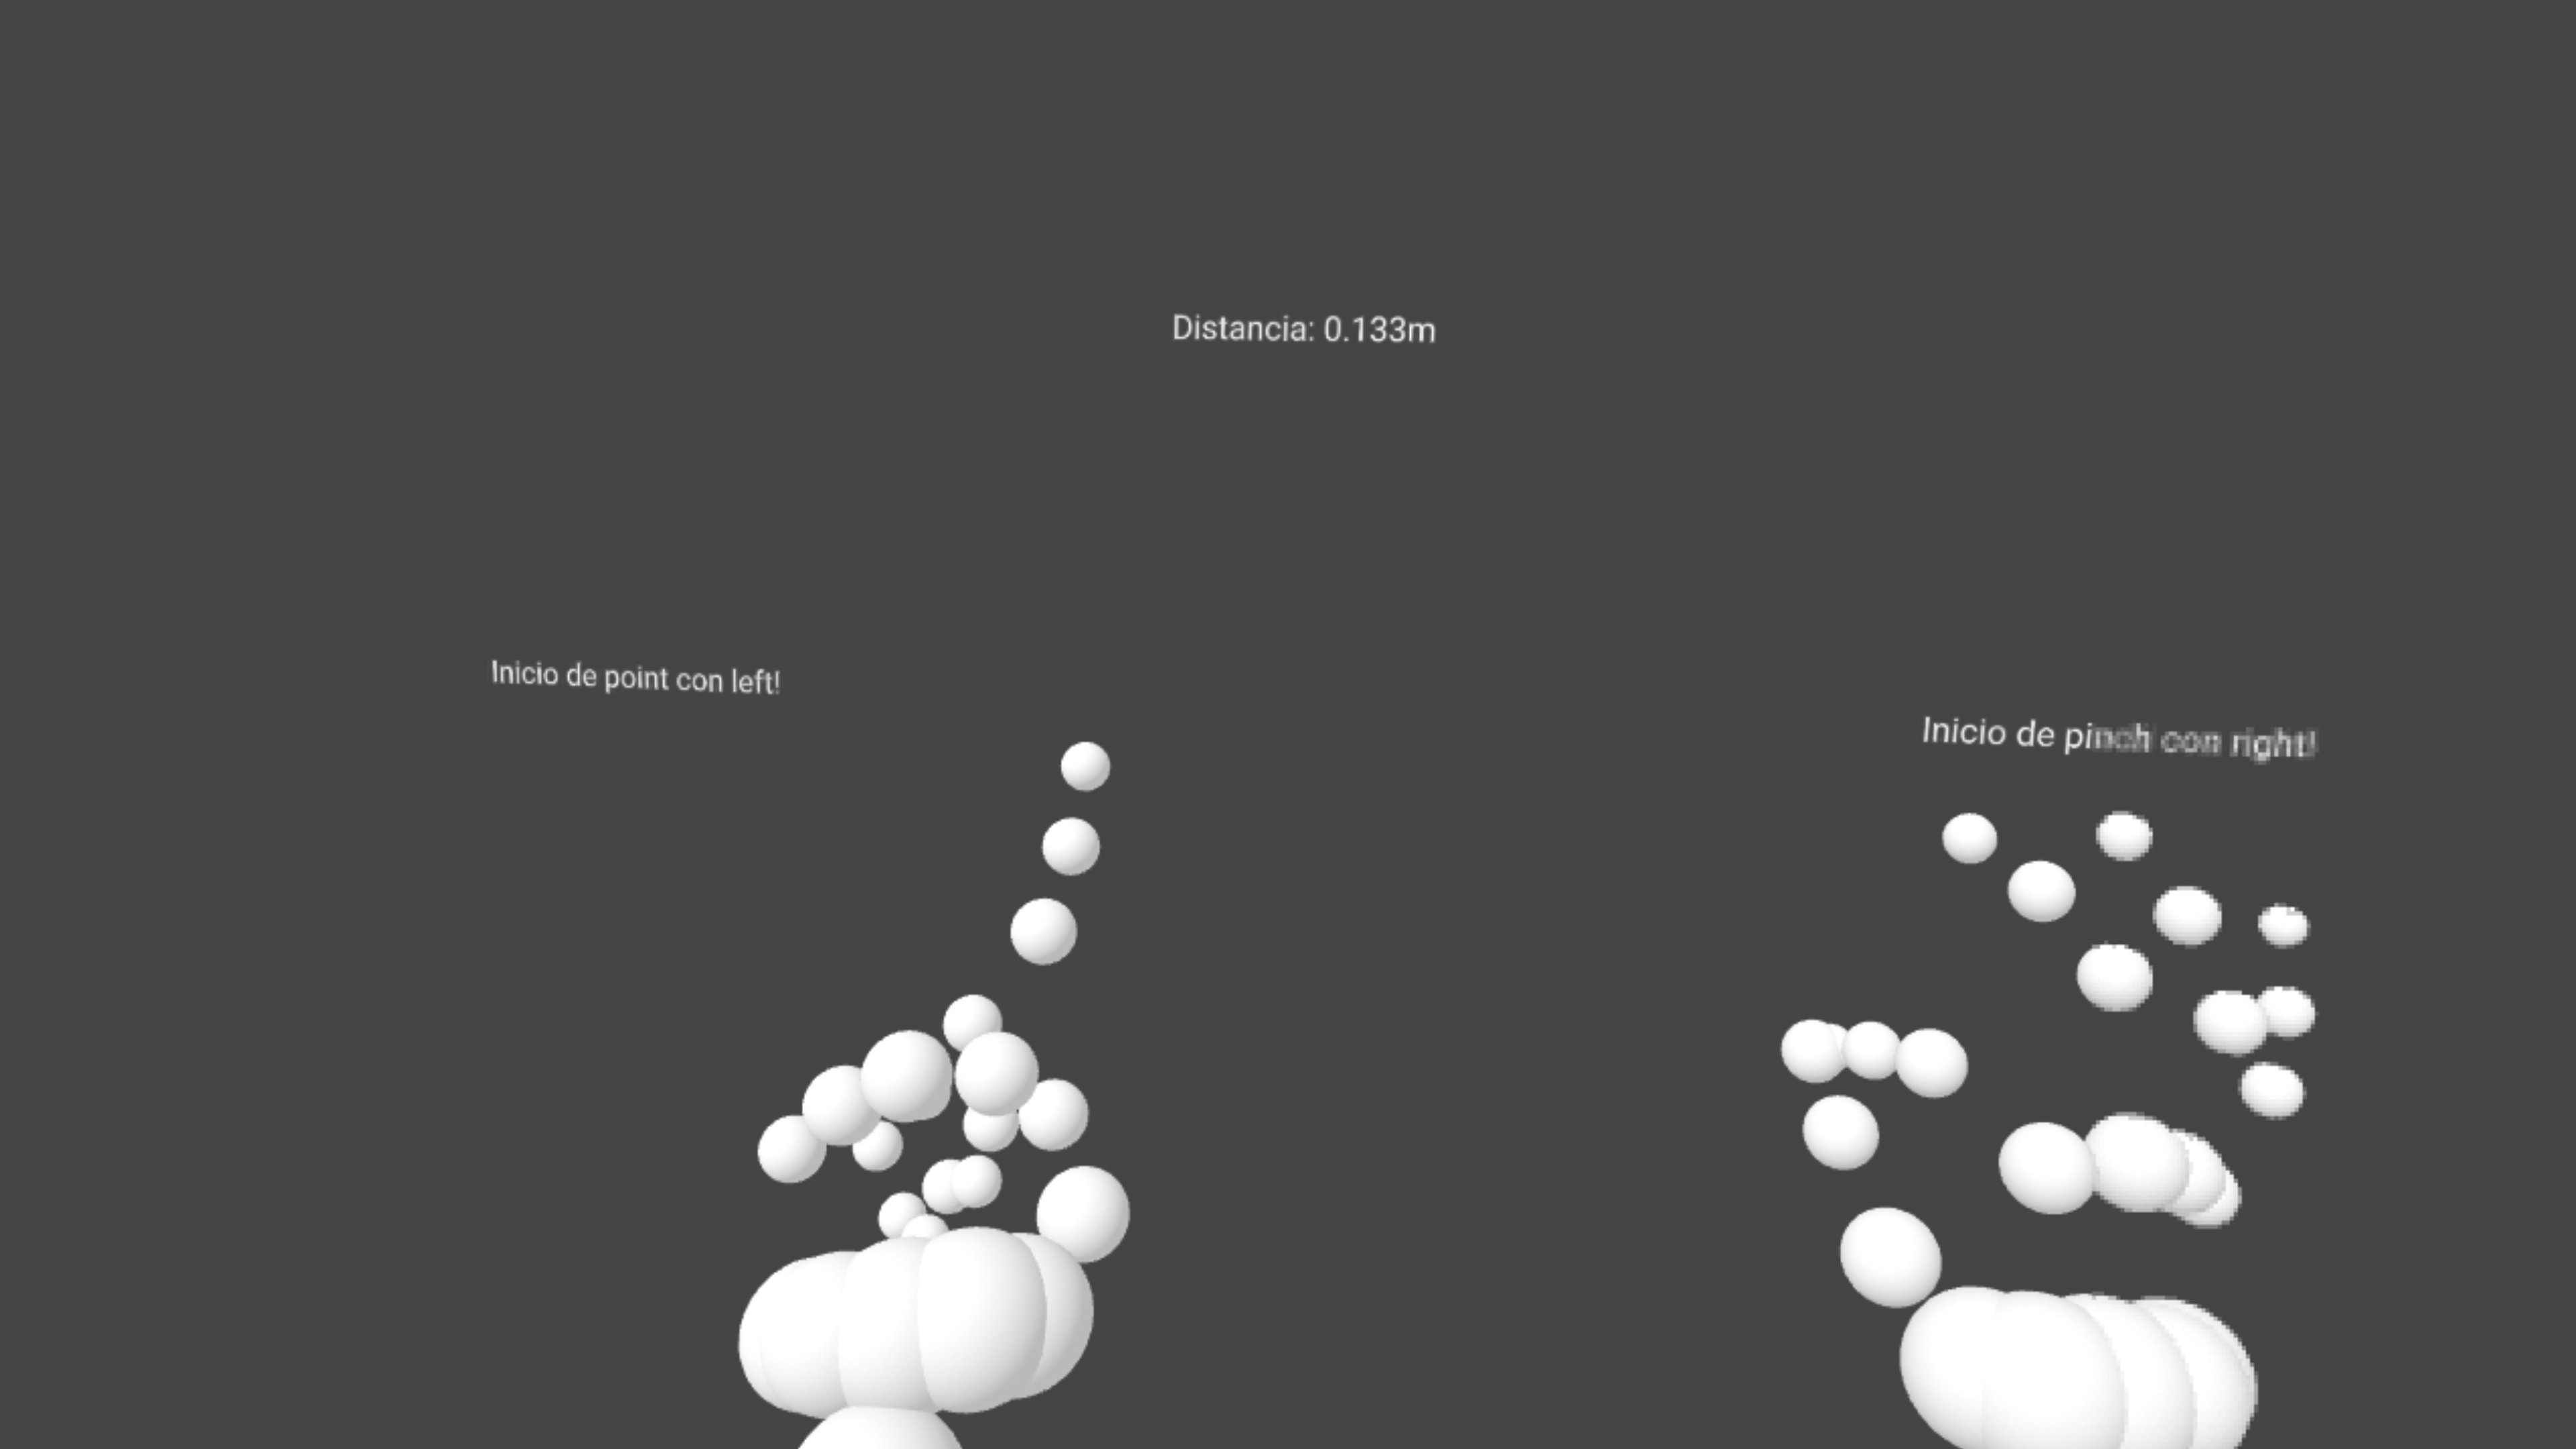
\includegraphics[width=0.7\textwidth]{img/nuevos_gestos.jpg} 
  % \fbox{\rule{0pt}{150pt} \rule{0.7\textwidth}{0pt}} 
  \caption{Nuevos gestos en la escena}
  \label{fig:sprint3}
\end{figure}

El resultado fue bastante similar al del sprint anterior, pero con la principal diferencia de que se habían añadido más gestos a la lógica de las manos, como se aprecia en la figura \ref{fig:sprint3}

Ahora que teníamos una lógica de seguimiento de manos y de gestos, era tiempo de crear la lógica necesaria para poder interactuar con los elementos dentro de la escena, para lo cual, primero era necesario saber cuando las manos estaban colisionando con los elementos de la escena. 

\section{Sprint 4}
\label{sec:sprint4}
Incorporación de colliders a la escena para la detección de colisiones.

\subsection{Objetivos}
\label{subsec:objetivo-principal4}
Como último paso de preparación de las manos era necesario saber cuando las manos estaban interactuando con los elementos de la escena. El objetivo principal de este sprint era la incorporación de colliders  
a la escena y preparar la lógica necesaria para poder detectar las colisiones entre los elementos de la escena. 

\subsection{Tareas Realizadas}
\label{subsec:implementacion4}
Para añadir Incorporación de colliders  
a la escena se hizo uso del componente propio de A-Frame, \textit{obb-collider}\footnote{\url{https://aframe.io/docs/1.7.0/components/obb-collider.html}}.
La principal ventaja que nos proporciona el uso de este componente nativo de A-Frame, era que cuando detecta una colisión entre 2 entidades que posean dicho componente, este lanza un evento indicando el inicio de la colisión y cuando no hay colisión lanza otro indicando el final de la colisión.
Los eventos que lanza el componente eran \texttt{obbcollisionstarted} y \texttt{obbcollisionended}.

Lo principal para añadir los colliders a la escena 
era añadirlos a la mano, ya que añadirlos a los distintos elementos de la escena era tan sencillo como añadir el componente de \texttt{obb-collider}. Para ello,
había que modificar la función encargada de actualizar las articulaciones de las manos. 

Dentro de la función de \texttt{updateSkeleton} \ref{lst:nuevas_manos} se añade las siguientes líneas de código:

\begin{lstlisting}[caption=Añadir Incorporación de colliders a la mano, captionpos=b, label=lst:colliders]
  
  if (!jointEntity.hasAttribute('obb-collider')) {
    jointEntity.setAttribute('obb-collider', `size: ${radius * 2} ${radius * 2} ${radius * 2}`);
  }
\end{lstlisting}

Como se aprecia en el código \ref{lst:colliders}, se comprueba si la articulación en cuestión tiene ya un collider y si no lo tiene, lo añade.

\subsection{Resultados}
\label{subsec:resultados4}
Como resultado de este sprint se obtuvo la demo de \textit{colliders}\footnote{\url{https://github.com/JuJoarias/TFG/blob/main/first_steps/second_hands/colliders.html}}. 

\begin{figure}[H] 
  \centering
  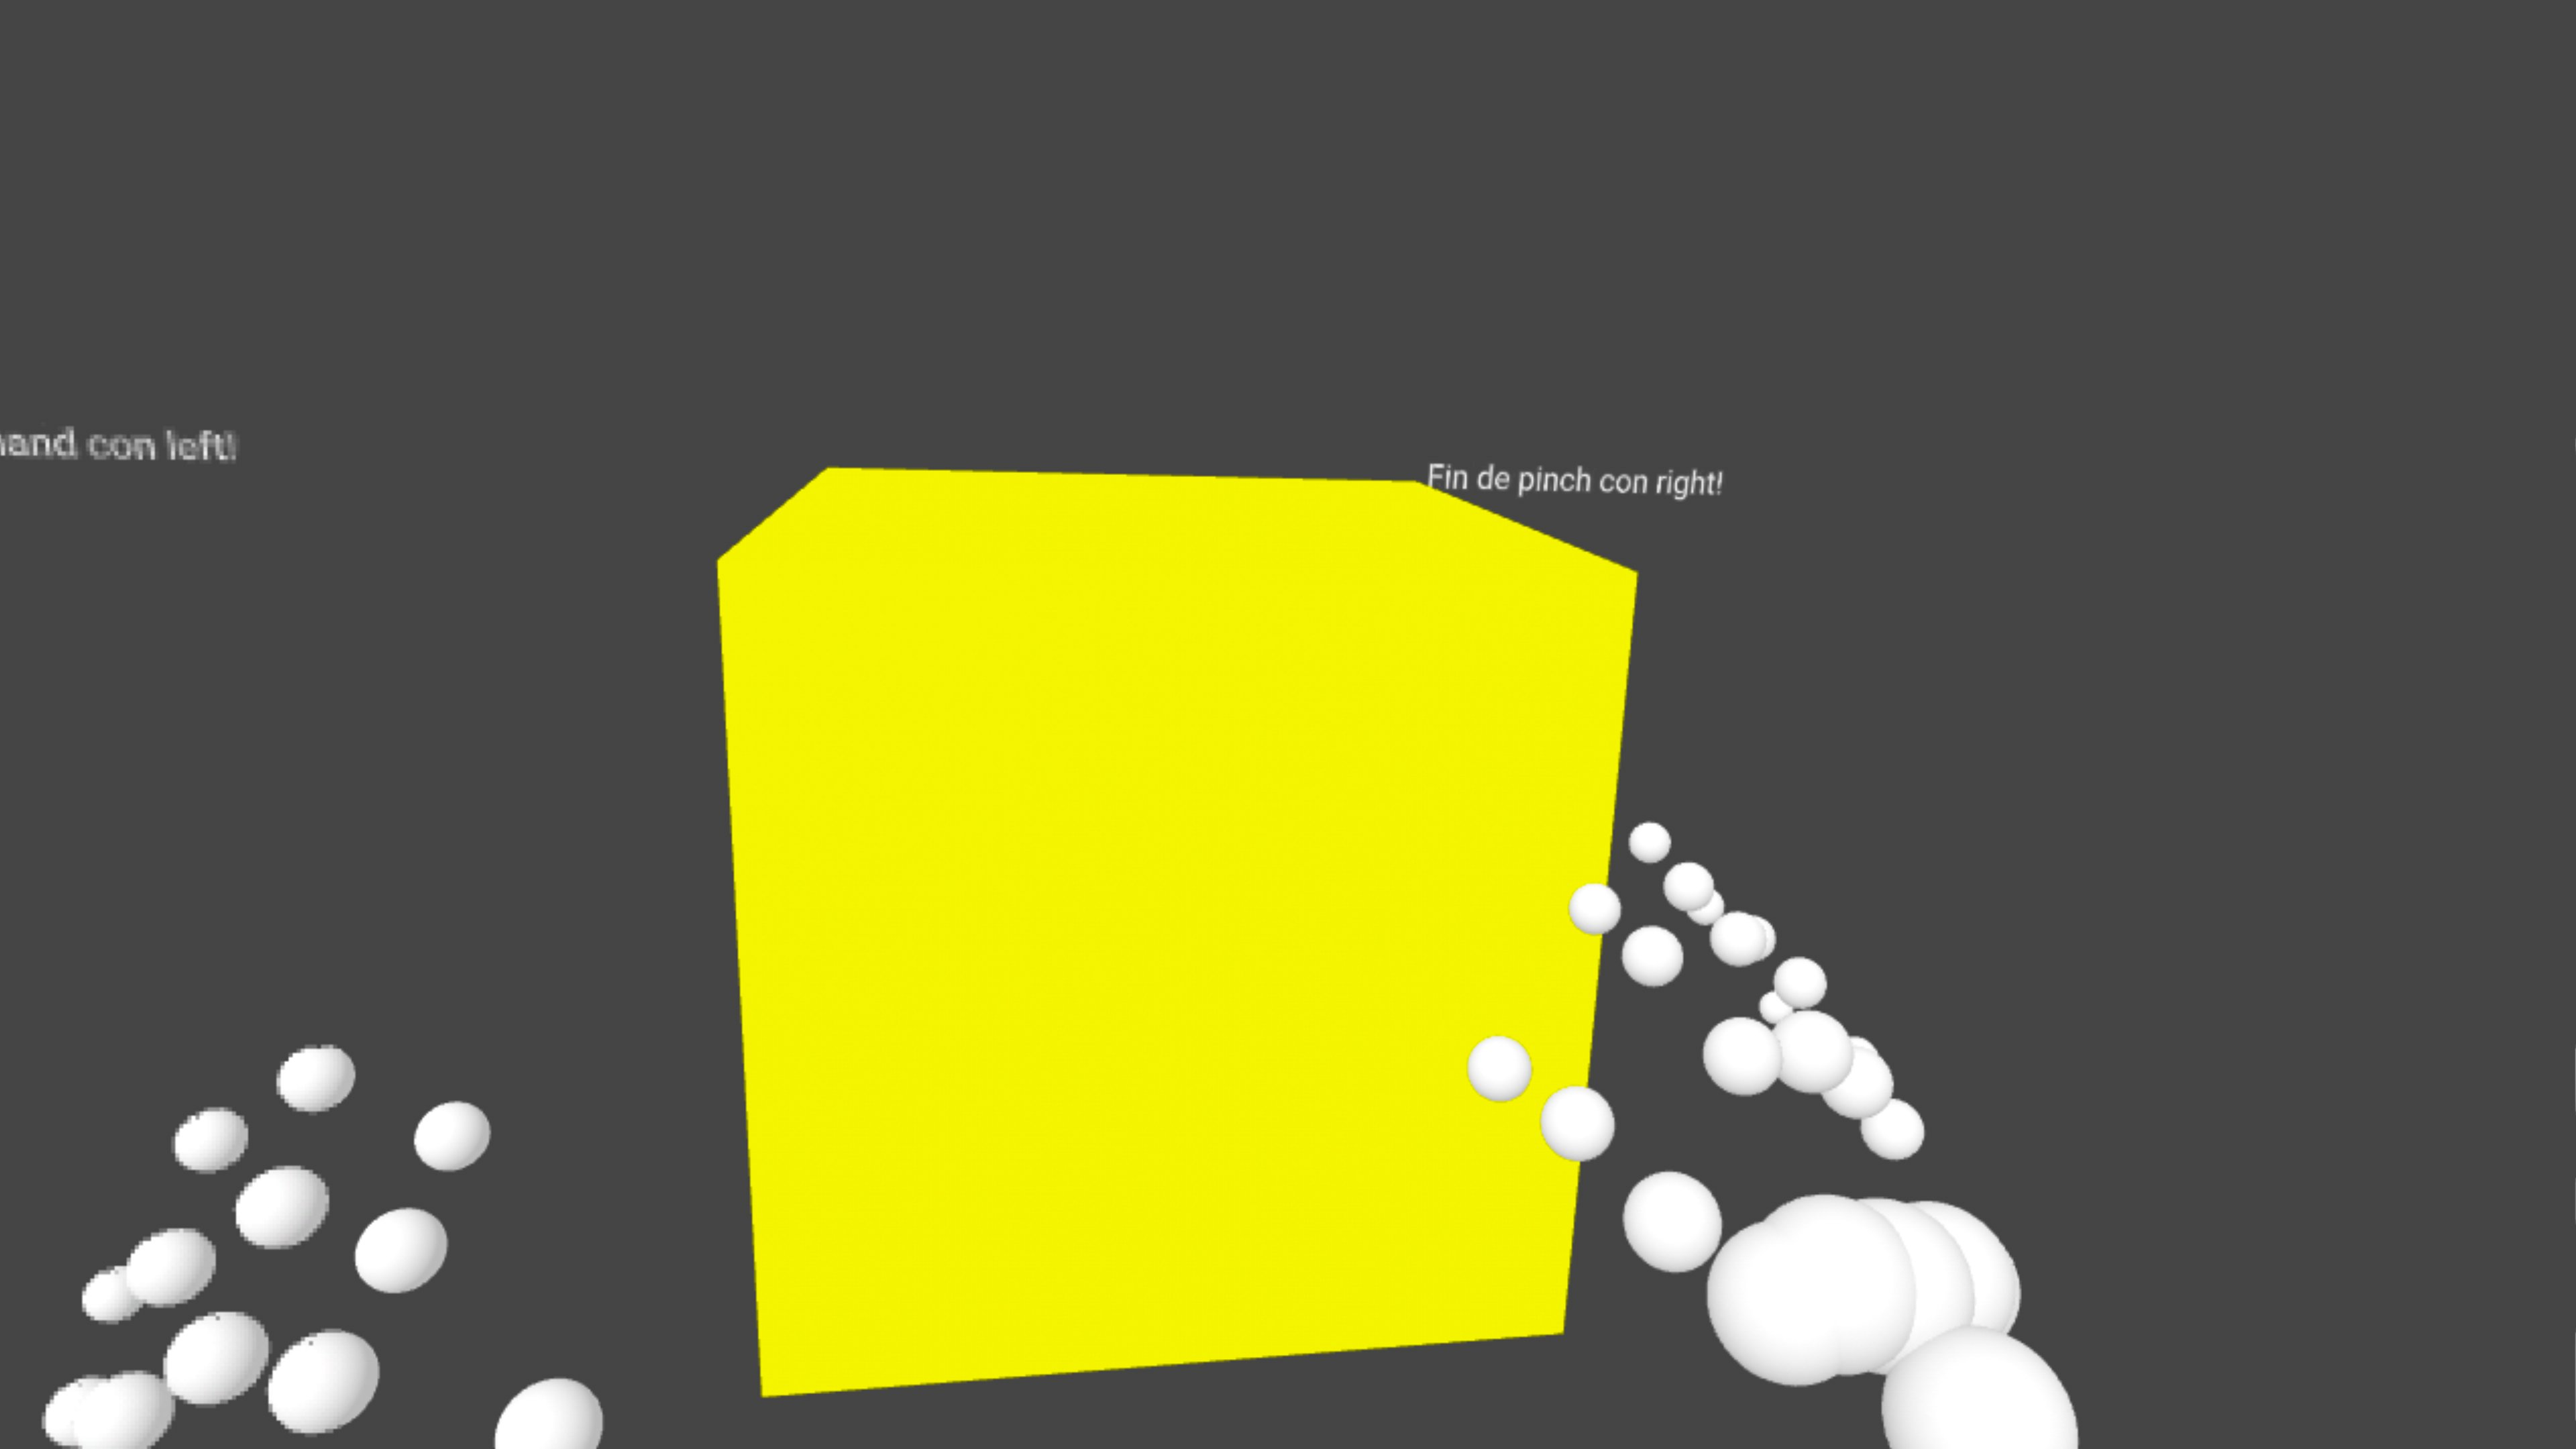
\includegraphics[width=0.7\textwidth]{img/collider.jpg} 
  % \fbox{\rule{0pt}{150pt} \rule{0.7\textwidth}{0pt}} 
  \caption{Demo colliders}
  \label{fig:sprint4}
\end{figure}

En dicha escena se mantienen los logros que ya habíamos obtenido en los sprints anteriores. Y para comprobar el funcionamiento de los colliders se añadió a la escena un cubo
al que le añadimos el componente de \texttt{obb-collider}. En dicha escena se implemento la lógica de que si se detectaba colisión entre el cubo y las manos, el color del cubo cambiaria para tener una respuesta más visual. 

Mientras se comprobaba el funcionamiento se noto un error. Como la mano estaba formada por varias esferas con espacios entre medias, y cada esfera poseía un colliders, se emitían varias veces los eventos de inicio y fin de la colisión, incluso si no se sacaba la mano del cubo. 
Esto era un problema ya que estos eventos repetidos cuando no corresponden hacían que cualquier función implementada cuando se detecta colisión actúe de forma intermitente y, por lo tanto, errónea. Aunque este problema no fue identificado hasta el sprint siguiente. 

\section{Sprint 5}
\label{sec:sprint5}
Incorporación de la función grabable a la escena para interactuar con los elementos.

\subsection{Objetivos}
\label{subsec:objetivo-principal5}
Para este sprint se quiso ya ir incorporando el funcionamiento de los gestos en la escena. Para empezar se quiso trabajar con el gesto \texttt{Pinch}. Se planteo que sí se hacía con la mano derecha sobre el cubo poder 
arrastrar dicho cubo por la escena en cualquier dirección e imitando la rotación de la mano para que parezca que lo estamos agarrando realmente. Y si se hacía con la mano izquierda, el cubo únicamente se podría deslizar en un único eje, el eje X.

\subsection{Tareas Realizadas}
\label{subsec:implementacion5}
Este sprint fue uno de los más complejos hasta ahora, ya que a lo largo del proceso fuimos encontrando distintos problemas que hicieron replantear la lógica del código. 

Para empezar con este sprint, se creo el componente de \texttt{Grabable}, dicho componente no posee un \texttt{schema}. Y en su init aparte de definir las distintas variables necesarias, se comprueba si la entidad a la que se añada el componente posee un collider, y en caso de no tener le añade uno.
En este componente toda la lógica se ejecuta dentro la una función llamada \texttt{check}, la cual se llama en el \texttt{tick}. 

En dicha función, lo primero que se comprueba es si hay una colisión, y si la hay ocurren 2 procesos importantes. El primero es que se cambia el estado de una variable booleana, la cual indica si hay colisión o no, y el segundo, se ejecuta una función llamada \texttt{hoover}. En esa función, para saber de forma visual que estamos interactuando con el cubo, incluso antes de realizar ningún gesto, se cambia la trasparencia del cubo ligeramente.

Para poder realizar correctamente la lógica del gesto, era necesario poder acceder a la información de las entidades que forman las articulaciones. Para ello, debíamos de ser capaces de acceder a la información del componente \texttt{manos} mediante las siguientes líneas de código:

Luego, para distinguir entre el pinch de la mano derecha y la mano izquierda, primero accedemos a la información de la mano derecha y de la izquierda a través del componente \texttt{manos}, esto lo hacemos accediendo a la información del componente como se muestra en el fragmento de código \ref{lst:info_manos}. Una vez con acceso a esa información, pudiendo distinguir las manos, se comprueba la variable de estado \texttt{pinchState}, la cual guardamos en dos constantes, una por cada mano. Estas constantes son las que nos proporcionan la información de si se está realizando el gesto y que mano lo está haciendo.

\begin{lstlisting}[caption=Acceso información componente manos, captionpos=b, label=lst:info_manos]
  
  this.leftHandEntity = document.querySelector('#left-hand');
  this.rightHandEntity = document.querySelector('#right-hand');

  const manoDerecha = this.rightHandEntity.components.manos;
  const manoIzquierda = this.leftHandEntity.components.manos;

  const rightPinchState = manoDerecha.pinchState;
  const leftPinchState = manoIzquierda.pinchState;
\end{lstlisting}

Con eso ya somos capaces de acceder a la información de \texttt{joints}, donde se almacenaban todas las entidades de las articulaciones.

Para la mano izquierda fue más sencillo. Se comprobaba si había colisión con el cubo y también si la variable correspondiente al pinch de la mano izquierda estaba en True, y de estarlo, el cubo cambiaba su color a azul y posteriormente se accede a la información 
de la punta del índice de la mano izquierda y se hace que el cubo copie la coordenada de dicha articulación mientras mantiene sus otras coordenadas, así se desliza únicamente en un único eje.

Para la mano derecha fue más complejo. Se quería poder agarrar el cubo y poder deslizarlo y rotarlo a antojo del usuario. Para ello se planteo hacer un \texttt{reparenting}, para volver la entidad del cubo hija de la entidad de la mano, para que así imitara sus movimientos y rotaciones. Para realizar esto se realizo un \textit{test externo}\footnote{\url{https://github.com/JuJoarias/TFG/blob/main/external_tests/reparenting_test.html}}.
El test dio los resultados deseados, pero a la hora de aplicarlo al código resaltaron varios problemas. 

El primero, era que no se lograba realizar el \texttt{reparenting} con la entidad de la mano, así que para solucionarlo se optó por que el nuevo padre del cubo fuese la punta del dedo índice mientras se realizaba el gesto.
Otro fallo que resalto fue la rotación. Pese a que el \texttt{reparenting} se realizaba correctamente, el cubo no seguía las rotaciones de la mano. Y esto se debía a como se dibujaban las manos, ya que a cada frame se actualiza la posición de cada articulación, pero no la rotación, con lo cual esta se mantiene fija. Para solucionar este problema, se optó por tomar 3 articulaciones de la mano y con estas 
como referencia para los ejes X y Z se creo un eje de coordenadas relativo. Dicho eje relativo seguiría la orientación y rotación de la mano. Una vez obtenido ese eje, cuando se realiza el gesto derecho, el cubo empieza a imitar dicho eje, permitiendo que el cubo rote al mismo tiempo que se arrastra el cubo por la escena. 

\subsection{Resultados}
\label{subsec:resultados5}
El resultado de este sprint se refleja en la demo \textit{hands grabable}\footnote{\url{https://github.com/JuJoarias/TFG/blob/main/first_steps/second_hands/hands_grabable.js}}. 

\begin{figure}[H] 
  \centering
  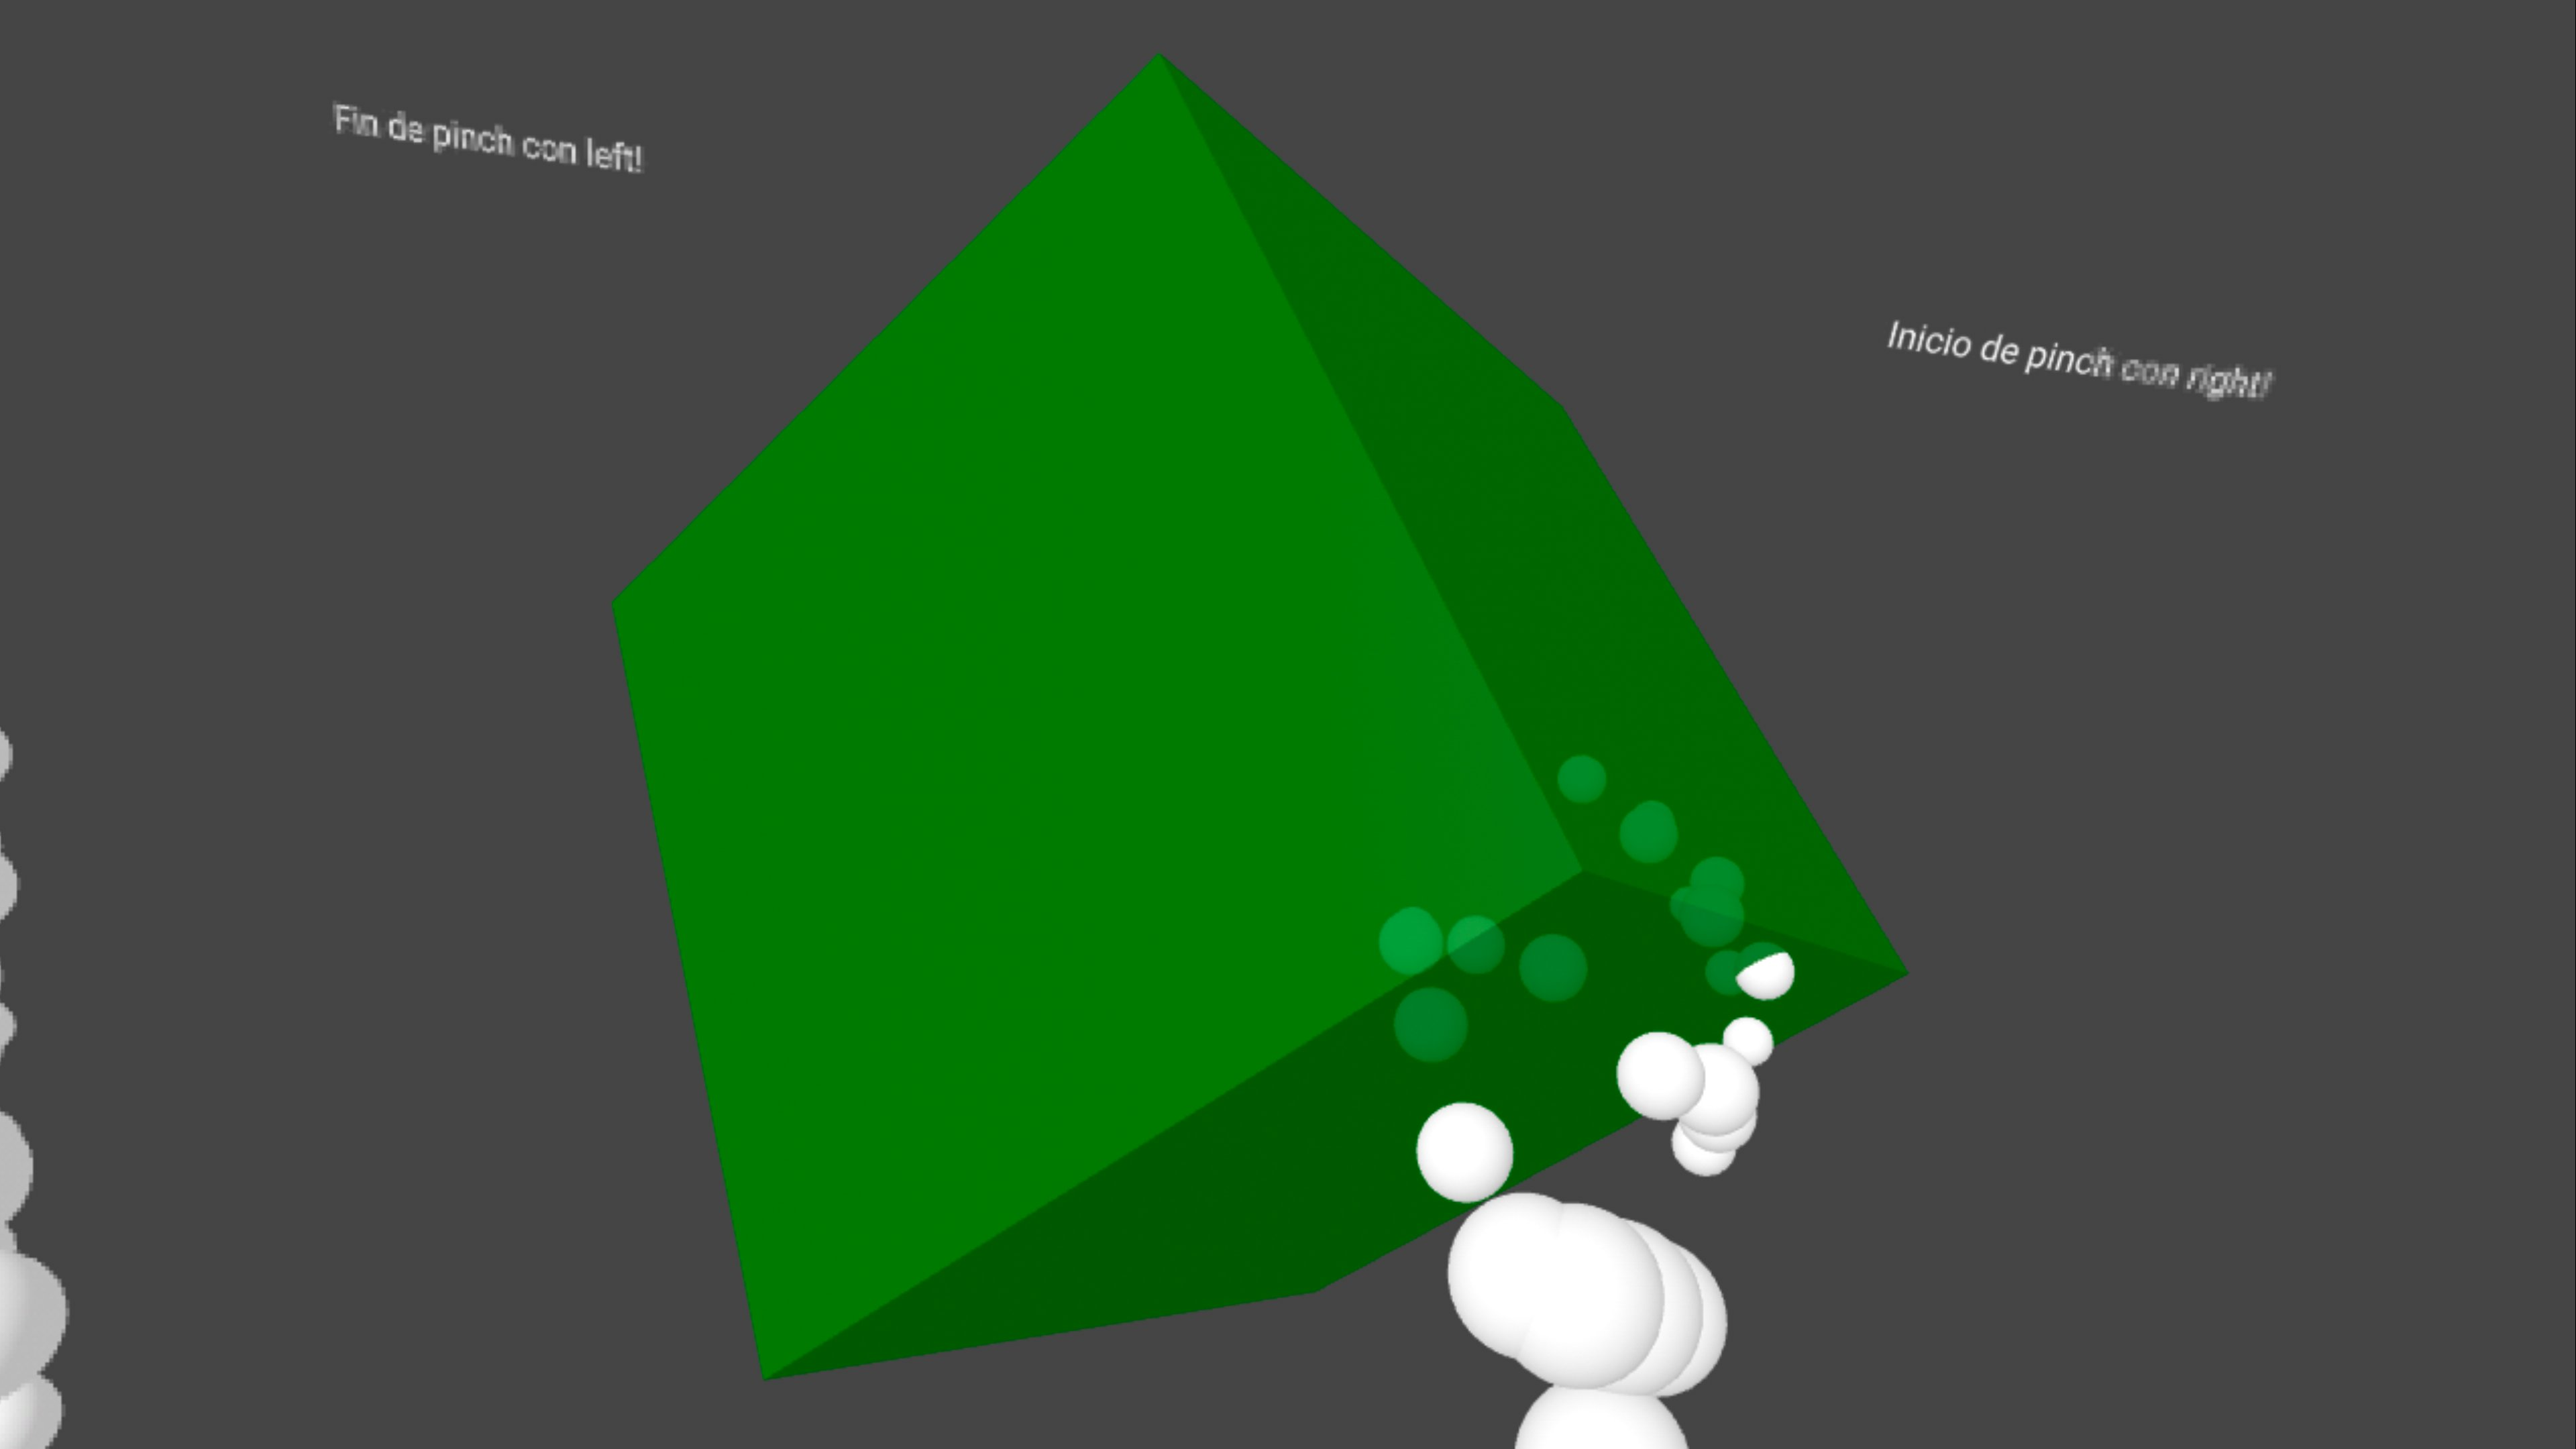
\includegraphics[width=0.7\textwidth]{img/grabable_right.jpg} 
  % \fbox{\rule{0pt}{150pt} \rule{0.7\textwidth}{0pt}} 
  \caption{Manos Grabable derecha}
  \label{fig:sprint5-1}
\end{figure}

\begin{figure}[H] 
  \centering
  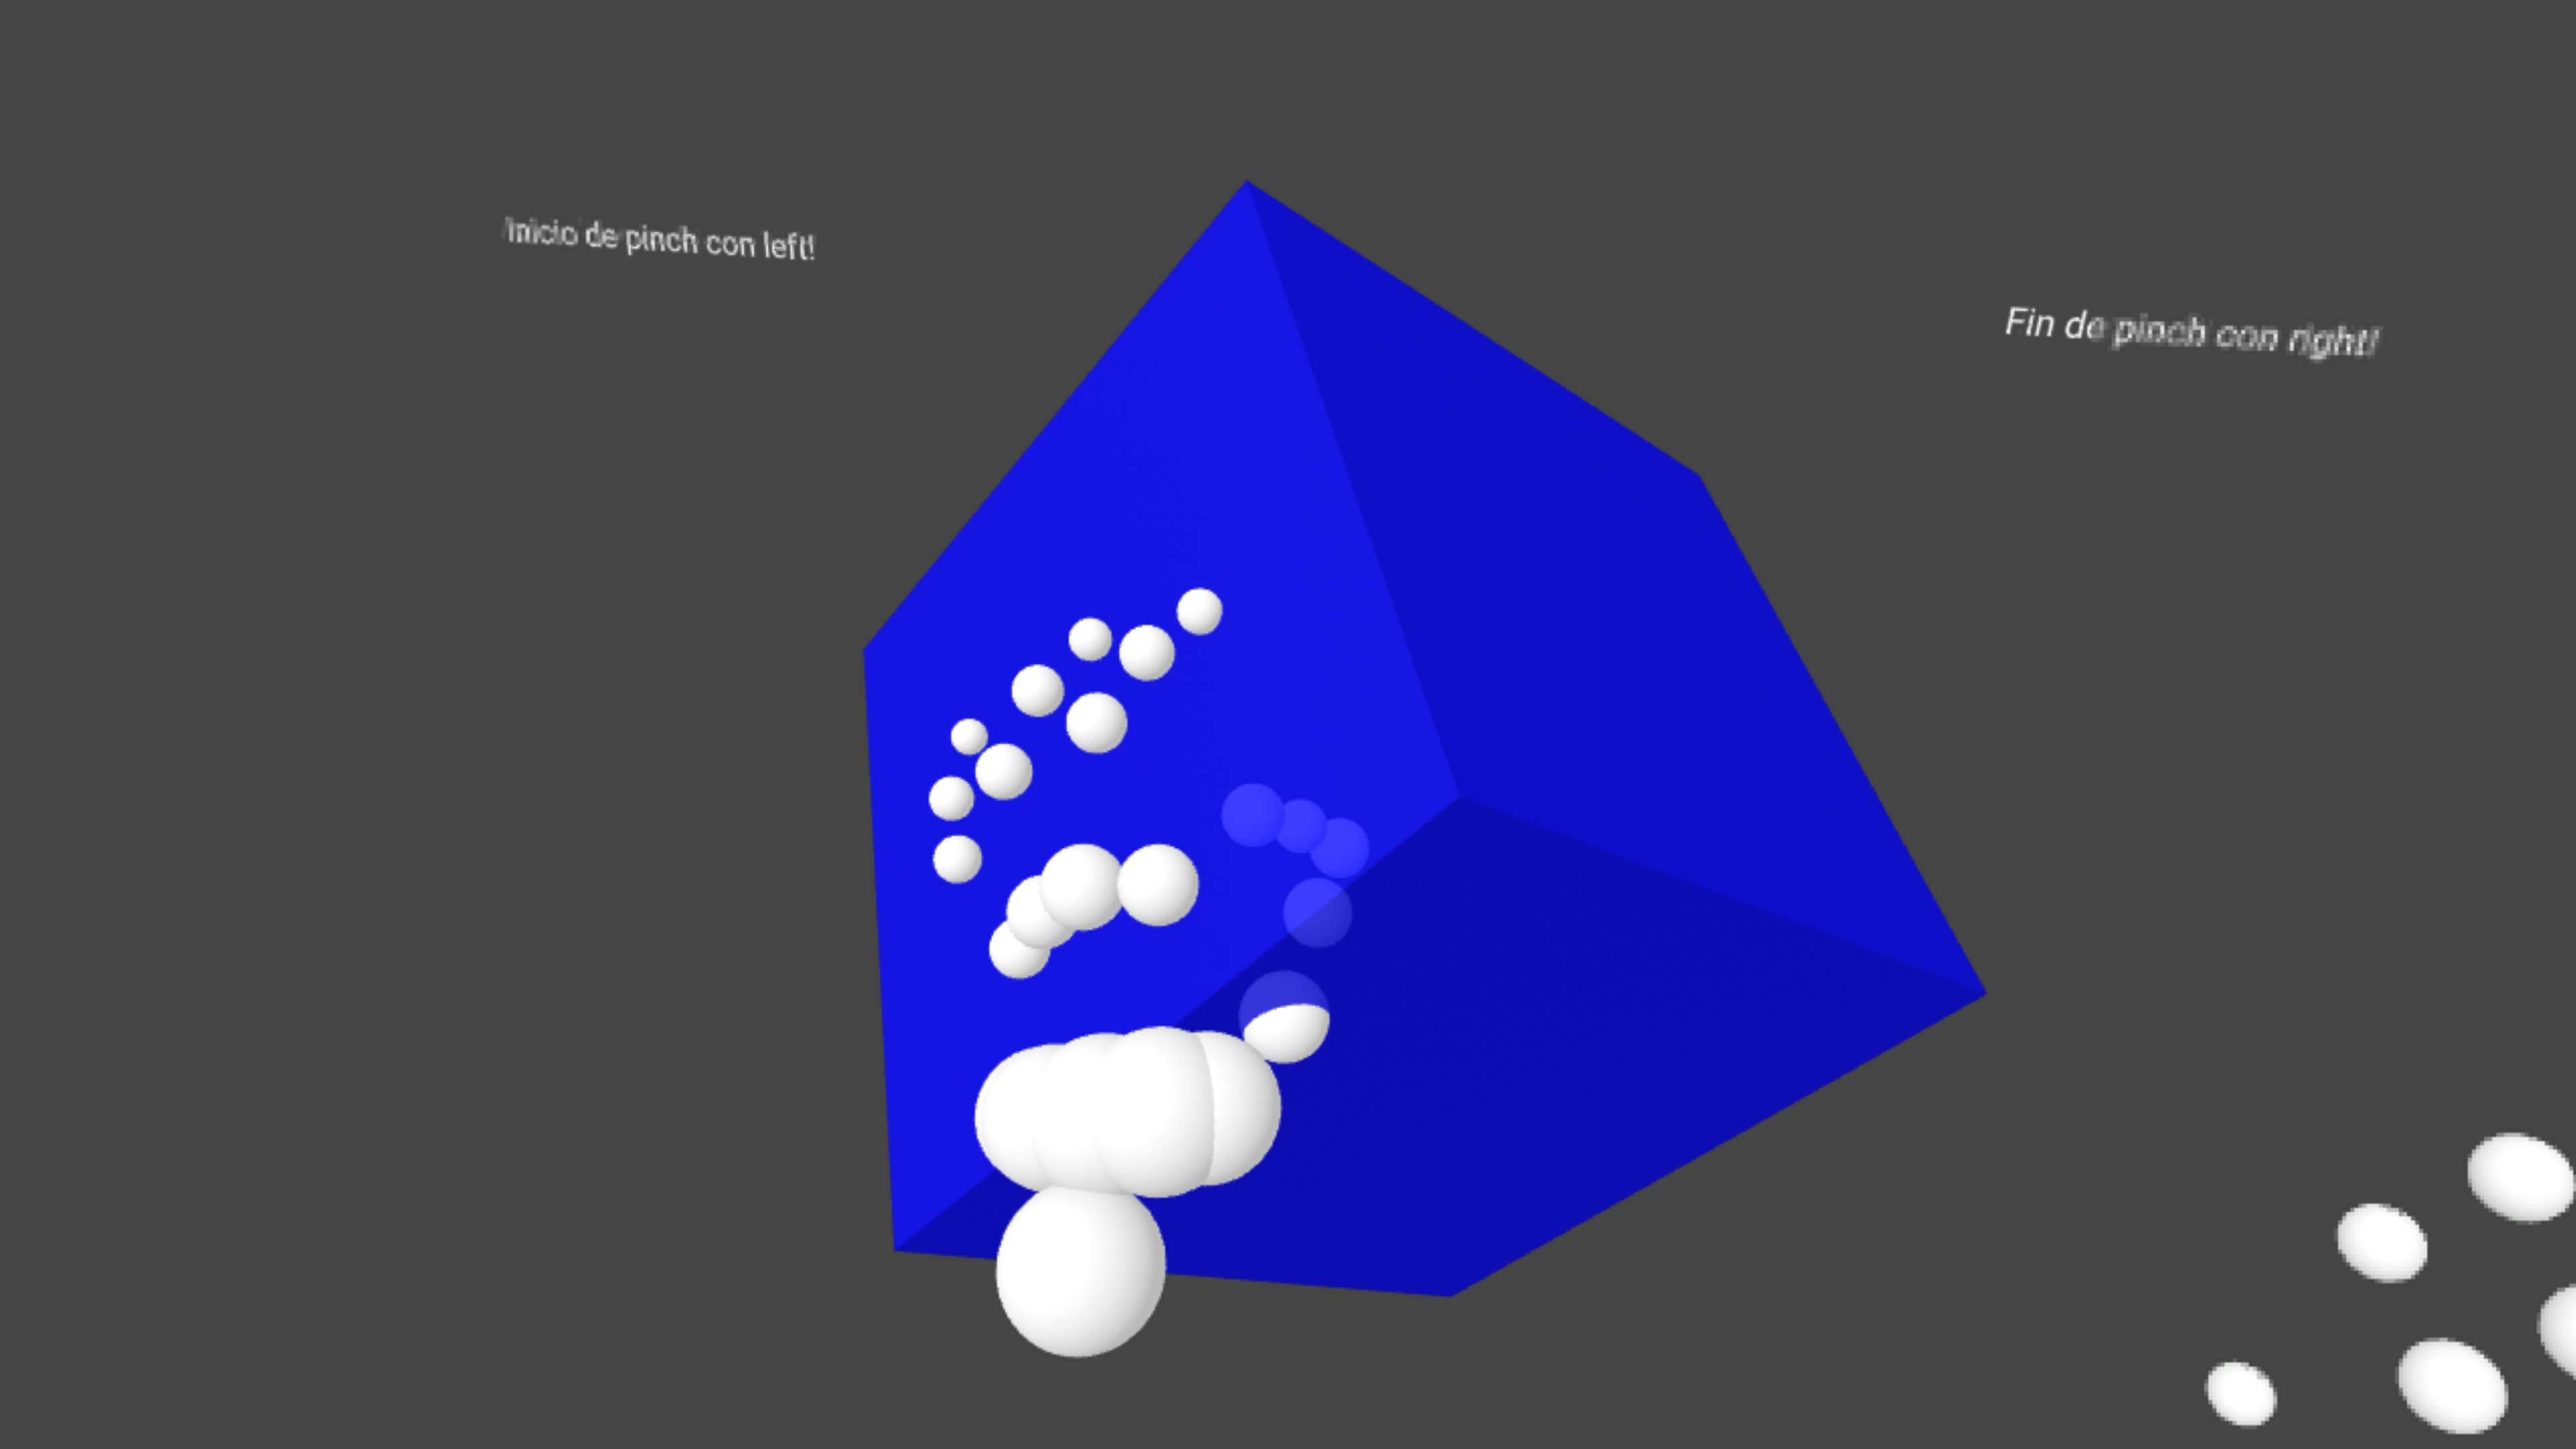
\includegraphics[width=0.7\textwidth]{img/grabable_left.jpg} 
  % \fbox{\rule{0pt}{150pt} \rule{0.7\textwidth}{0pt}} 
  \caption{Manos Grabable izquierda}
  \label{fig:sprint5-2}
\end{figure}

Como se aprecia en las figuras \ref{fig:sprint5-1} y \ref{fig:sprint5-2} cada vez que se realiza el gesto con cada una de las manos sobre el cubo, este reacciona de manera distinta. 
El color cabía para tener una respuesta más visual, además de que cada mano tenía sé propia reacción. 

Con esto se había conseguido implementar las acciones de \texttt{Hoover}, \texttt{Drag} y \texttt{Slide}. De cara al siguiente sprint se decidió organizar mejor el código de dichas acciones al igual que añadir las acciones de \texttt{Stretch} y \texttt{Click}

\section{Sprint 6}
\label{sec:sprint6}
Creación de las manos finales del proyecto, optimización de elementos y cierre del proyecto.

\subsection{Objetivos}
\label{subsec:objetivo-principal6}
El objetivo de este último sprint era añadir nuevas acciones y organizar mejor el código para que quedase lo más limpio posible. 
También, por sugerencia del tutor, se intento modificar el código para que las manos diseñadas en este proyecto funcionasen junto con el componente ya existente de \texttt{Superhands}, aunque esto no se logro al final. 

\subsection{Tareas Realizadas}
\label{subsec:implementacion6}
Para empezar con este sprint, primero se decidió por organizar el código ya existente y las acciones. Para ello, por cada acción que ya estaba implementada, \texttt{Hoover}, \texttt{Drag} y \texttt{Slide}, se creo un componente. También, el componente \texttt{Grabable}, creado en el sprint anterior, fue modificado para que en vez de llamar directamente a las funciones encargadas de las acciones de los gestos, emita los eventos \texttt{Start} o \texttt{End} correspondientes a cada acción. 

Dichos eventos luego serían escuchados por el componente correspondiente. La estructura de los componentes de las acciones todos siguen la misma estructura. En el \texttt{Init} primero se comprueba si la entidad a la que fue añadido contiene también el componente \texttt{Grabable} y si no lo tiene lo añade ya que este componente es indispensable para que los componentes de acciones funcionen a excepción del componente correspondiente al \texttt{Click}. Luego de eso, el componente escucha los eventos de \texttt{Start} y \texttt{End} y si los escucha, llama a una función
, la cual inicializa los datos o variables correspondientes que posteriormente se usaran en la función \texttt{Tick} del componente. En el siguiente fragmento de código se aprecia el componente \texttt{hoover} como ejemplo:

\begin{lstlisting}[caption=Componente Hoover, captionpos=b, label=lst:Hoover]
  
  AFRAME.registerComponent('hoover', {

    init: function(){
        if (!this.el.hasAttribute('grabable')) {
            this.el.setAttribute('grabable', '');
        }

       this.el.addEventListener('hooverStart', this.onHooverStart.bind(this));
       this.el.addEventListener('hooverEnd', this.onHooverEnd.bind(this));
       this.hooverState = false;
       this.isHoovering = false;
    },

    onHooverStart: function () {
       if (this.isHoovering) return;
       this.isHoovering = true;

       this.hooverState = true;
    },

    onHooverEnd: function () {
       this.hooverState = false;
       this.isHoovering = false;
    },

    tick: function () {
        if (this.hooverState){
           this.el.setAttribute('material', 'opacity', '0.8');
        } else{
           this.el.setAttribute('material', 'opacity', '1');
        }
    },
});
\end{lstlisting}

Para los componentes de \texttt{Slide} y \texttt{Drag} se ha mantenido la lógica obtenida en el sprint anterior, pero aplicando la estructura mostrada. 
También, al componente \texttt{Slide}, se le añadió un \texttt{Schema}. Este componente es el único que lo tiene y en él se puede definir en que eje queremos que se deslice el objeto, ya no se limita al eje X.

Respecto al componente de \texttt{Stretch}, la lógica detrás del gesto es similar a las acciones previamente implementadas. La única diferencia es que este componente únicamente reacciona cuando se está haciendo el gesto sobre el mismo objeto con ambas manos a la vez.
Una vez activado, el componente comprueba la distancia entre la punta de los dedos índices de ambas manos y con esa distancia la guarda en una variable. Utilizando esa distancia inicial, se crea un factor de escalado al dividir la distancia actual entre las manos y la inicial. Posteriormente, se multiplica dicho factor por la escala del objeto, así esta crecerá o decrecerá dependiendo de la distancia entre ambas manos. 

Hasta ahora todas las acciones habían funcionado con el gesto \texttt{Pinch}, pero para la acción de \texttt{Click} era necesario otro. Para este componente se utilizo el gesto de \texttt{Point}, el cual consistía en tener el dedo índice estirado. Al realizar el gesto el código crearía un puntero desde la punta del dedo y a cada frame actualizaría su dirección utilizando como vector la línea que une la punta del dedo con su nudillo. 
Ahora que teníamos el puntero era necesaria una acción para que se emitiera el evento. Para ello, se utilizó el dedo pulgar. Como si se tratase de una pistola, se configuró el código para que cuando se haga el gesto de "disparar una pistola" se emitiera el evento de click. Toda esta implementación del gesto se introdujo directamente dentro del componente principal, el componente \texttt{Manos}. 
Posteriormente, en el propio componente, al escuchar el evento, este componente únicamente cambia el color del cubo a morado y al soltar el gesto de pistola, sin necesidad de soltar el gesto de \texttt{Point}, el color vuelve a su color original. 

Aparte de eso, se realizo otra optimización. Hasta ahora, se habían añadido colisionadores a todas las articulaciones de la mano, pero esto resulto en varios problemas. El principal problema era que, ya que las articulaciones no se tocaban entre sí, cuando el usuario tocaba con la mano los elementos de la escena, los eventos del colisionador se repetían, esto se debía a que cada articulación estaba mandando los eventos, lo cual hacía que el resto de funcionalidades relacionadas a las acciones con la mano no funcionases correctamente. 
Para solucionar esto, se opto por limitar la cantidad de colisionadores en la mano a la punta del dedo índice y a la muñeca. Esta decisión se tomo ya que, para la mayoría de interacciones, únicamente con detectar la colisión del dedo índice es suficiente y en el caso de la muñeca, esto se hizo pensando en futuras implementaciones como por ejemplo pulsar un botón con la mano en vez de con un dedo.

\subsection{Resultados}
\label{subsec:resultados6}
El resultado de este sprint es la propia \textit{demo}\footnote{\url{https://github.com/JuJoarias/TFG/blob/main/demo/demo.html}} presentada al final. 

\begin{figure}[H] 
  \centering
  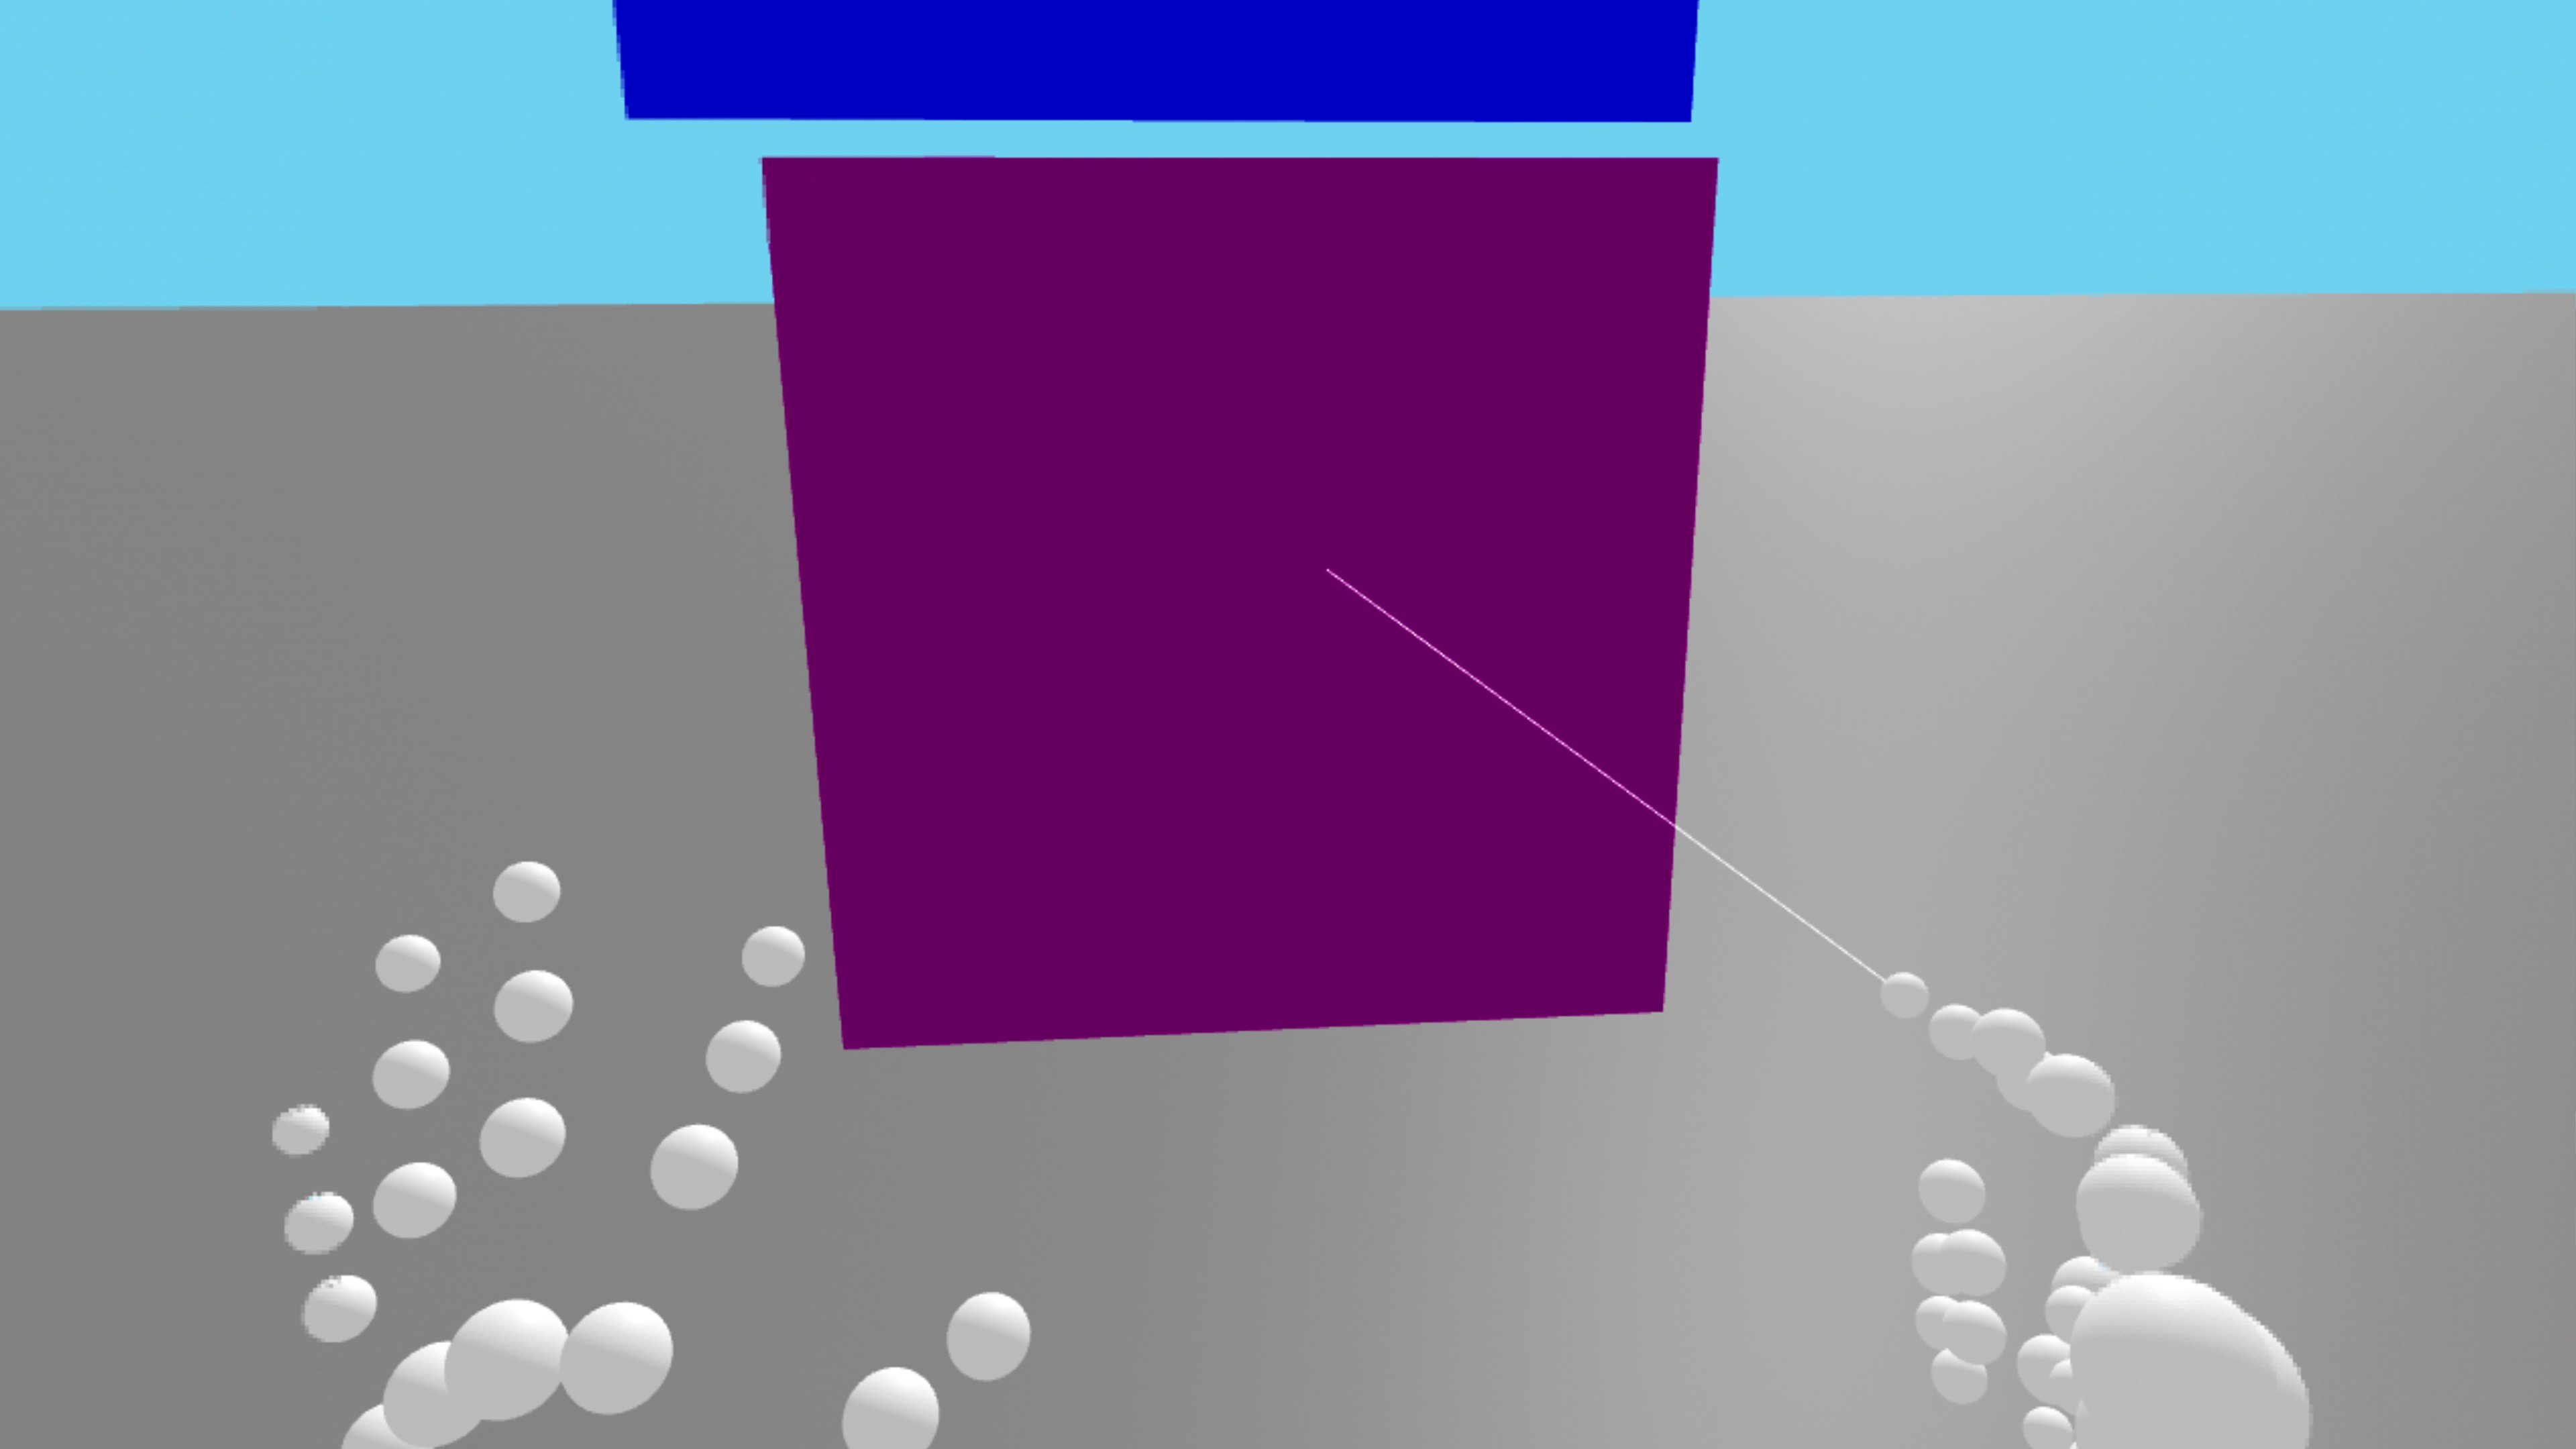
\includegraphics[width=0.7\textwidth]{img/click.jpg} 
  % \fbox{\rule{0pt}{150pt} \rule{0.7\textwidth}{0pt}} 
  \caption{Manos finales click}
  \label{fig:sprint6-1}
\end{figure}

\begin{figure}[H] 
  \centering
  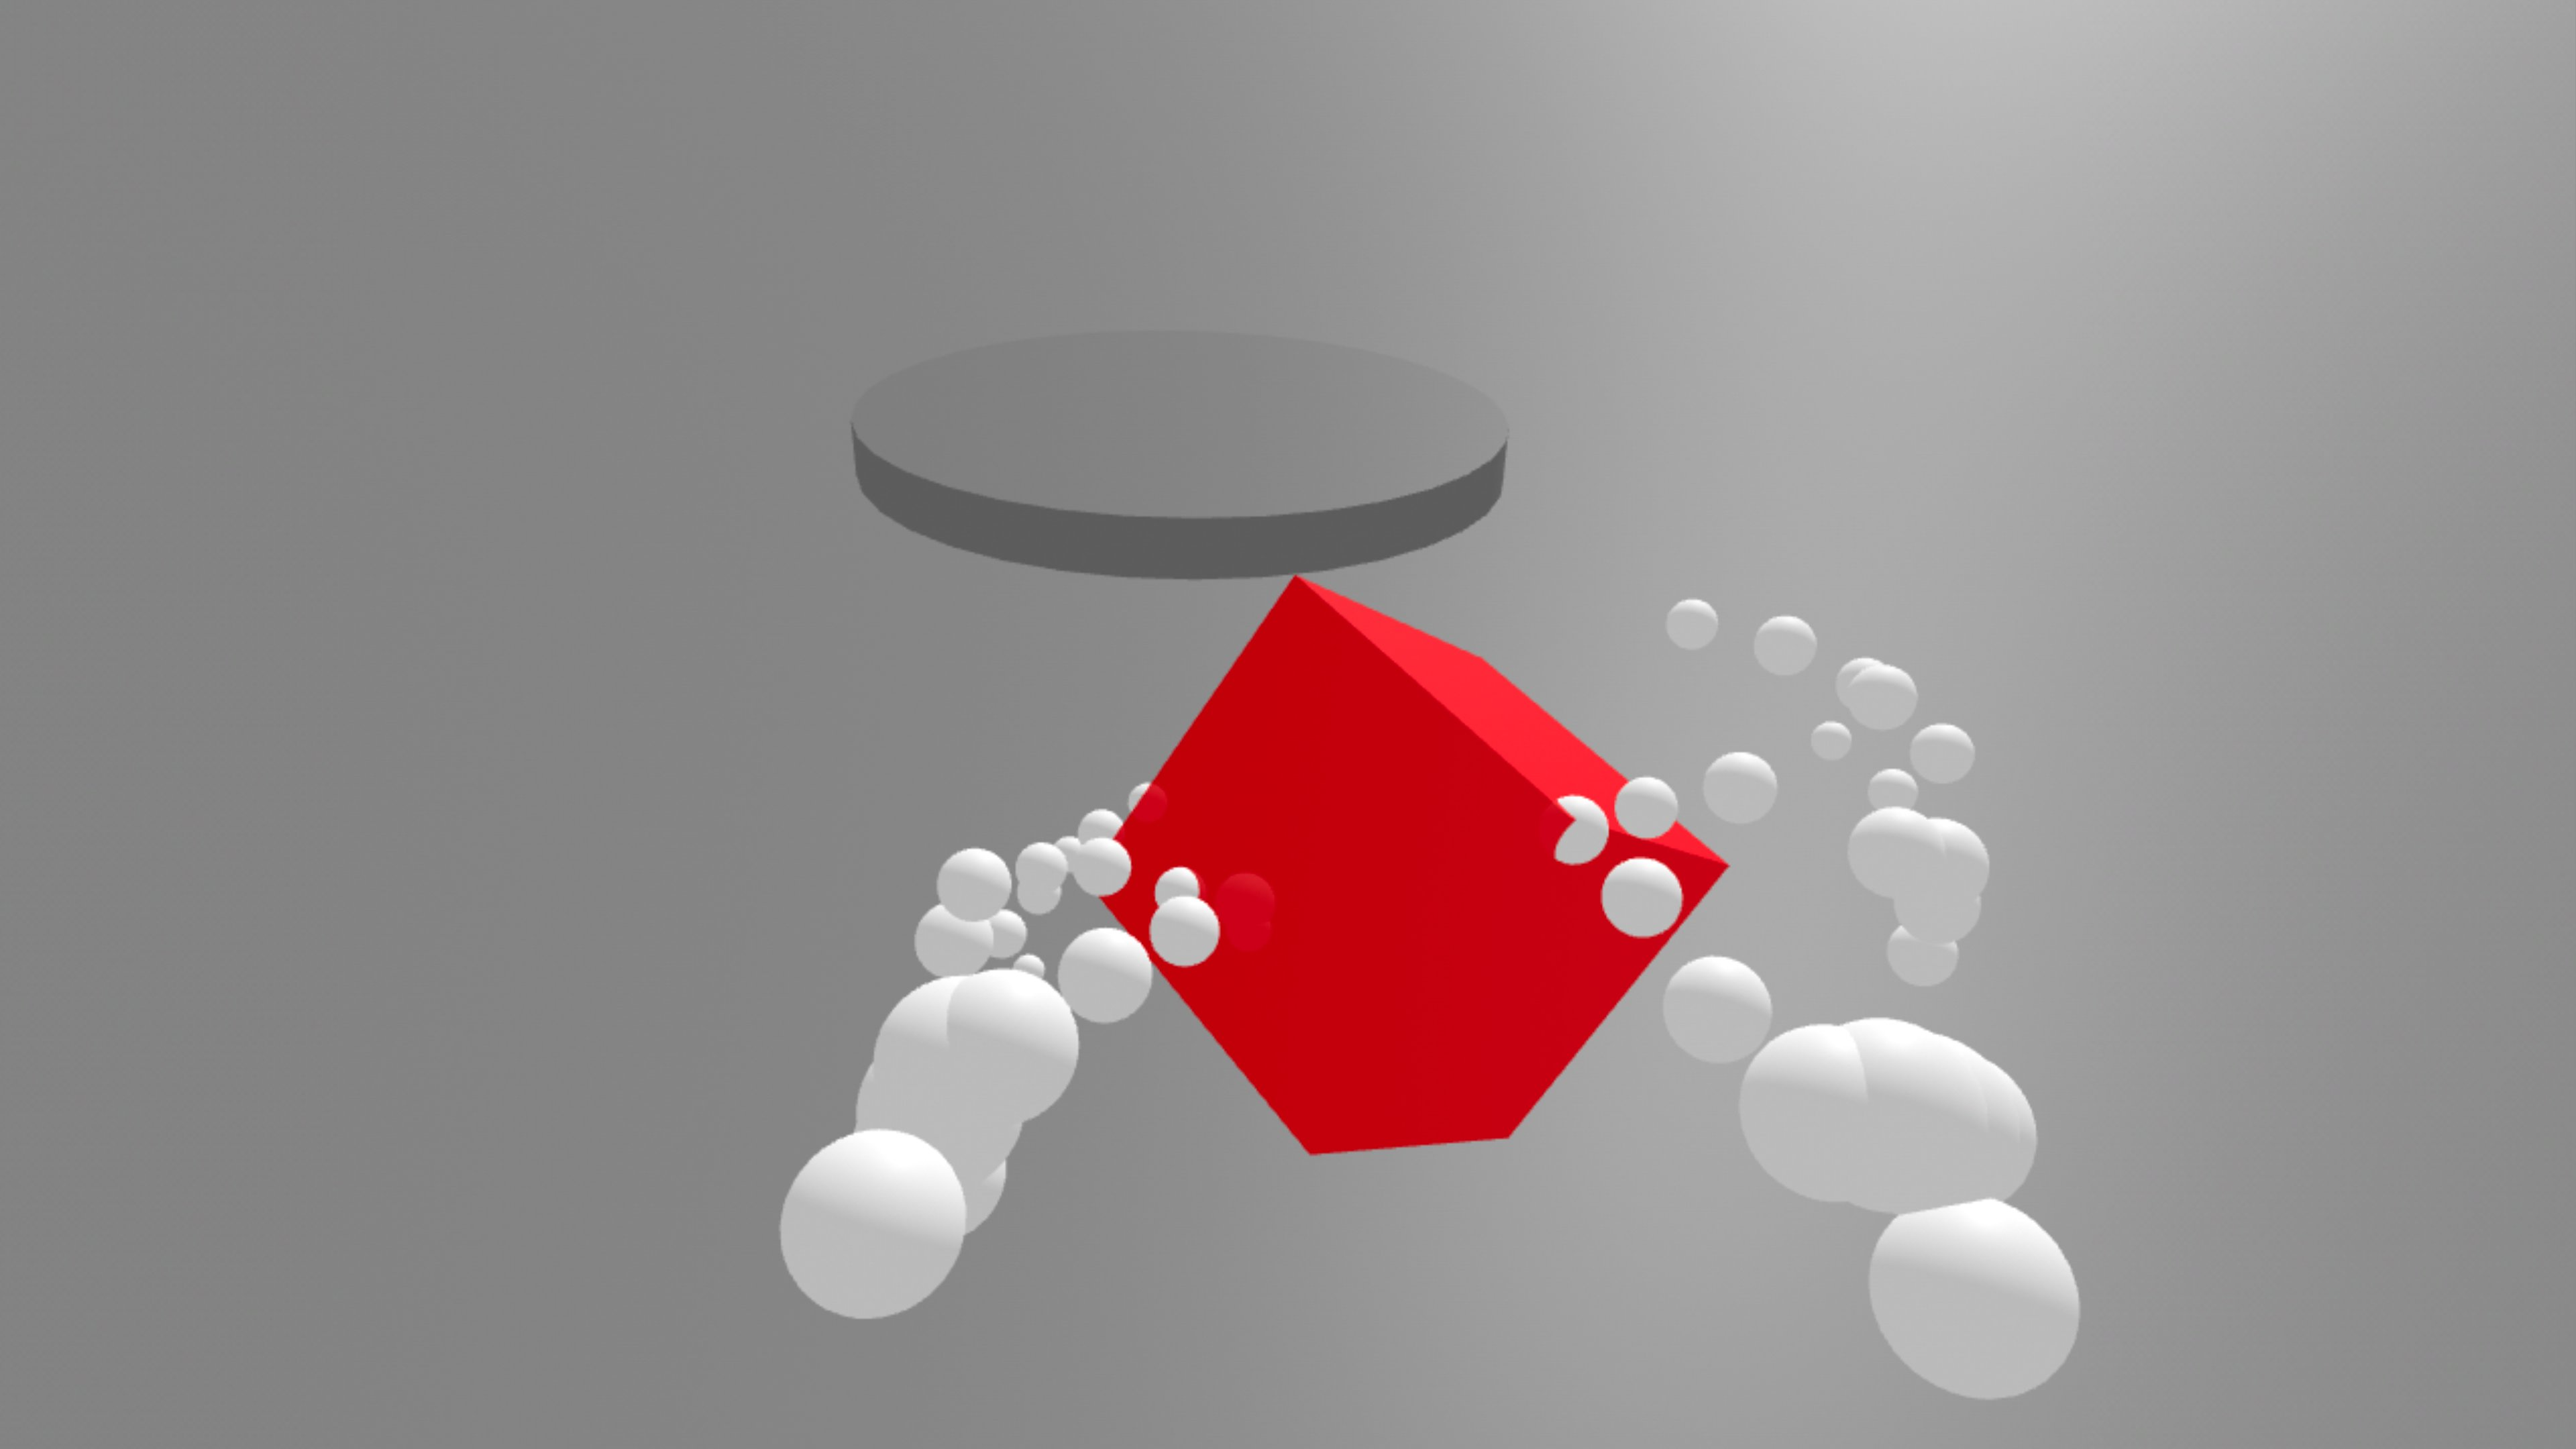
\includegraphics[width=0.7\textwidth]{img/stretch.jpg} 
  % \fbox{\rule{0pt}{150pt} \rule{0.7\textwidth}{0pt}} 
  \caption{Manos finales stretch}
  \label{fig:sprint6-2}
\end{figure}

En las figuras \ref{fig:sprint6-1} y \ref{fig:sprint6-2} se muestran algunas de las acciones implementadas durante este proyecto. En esta demo se aprecia un cubo por cada acción que se implemento al igual que un cubo que posee todas ya que cada cubo únicamente cuenta con uno de los componentes de acción.

%%%%%%%%%%%%%%%%%%%%%%%%%%%%%%%%%%%%%%%%%%%%%%%%%%%%%%%%%%%%%%%%%%%%%%%%%%%%%%%%
%%%%%%%%%%%%%%%%%%%%%%%%%%%%%%%%%%%%%%%%%%%%%%%%%%%%%%%%%%%%%%%%%%%%%%%%%%%%%%%%
% PRUEBAS Y EXPERIMENTOS capitulo 5%
%%%%%%%%%%%%%%%%%%%%%%%%%%%%%%%%%%%%%%%%%%%%%%%%%%%%%%%%%%%%%%%%%%%%%%%%%%%%%%%%

\cleardoublepage
\chapter{Pruebas y experimentos}
\label{chap:pruebas-experimentos}
En este capítulo se describirán las distintas impresiones que han tenido familiares y amigos que han ayudado al probar la escena final. 

Primero se describirán las condiciones en las que se desarrolló el experimento al igual que las distintas instrucciones que se les dieron a cada uno nada más entrar a la escena y posteriormente se describirán las distintas impresiones y opiniones que han dado al respecto, finalmente, se explicarán las reflexiones obtenidas a raíz de dichas opiniones.
Para este apartado se pidió la colaboración de 4 voluntarios.

A la hora de realizar el experimento de prueba, las condiciones fueron las siguientes: Para empezar, los 4 voluntarios que ayudaron con el experimento no tenían conocimientos sobre la programación y era su primera experiencia dentro de un entrono de realidad virtual. Se utilizó el dispositivo Quest3 y el experimento tuvo lugar en un cuarto amplio para que los usuarios pudieran caminar cómodamente hasta cada uno de los elementos de la escena.
Previamente a entregarles el dispositivo para que realicen la prueba, yo cargué la escena en el navegador del dispositivo y posteriormente se lo cedí a los voluntarios. La escena que probaron se trataba de la escena descrita en la \hyperref[subsec:demo-componentes]{sección 1.1 del capítulo 3}, donde hay una serie de elementos en la escena y cada uno de los elementos contiene uno de los distintos componentes que se han desarrollado a lo largo de este proyecto.

Una vez dentro de la escena, los usuarios recibieron las siguientes instrucciones para familiarizarse con esta: 

\begin{itemize}
  \item \textbf{Mirar sus manos y avisar cuando las vean.} Esto era para permitir que el sistema detectase las manos y pudiera renderizarlas dentro de la escena.
  \item \textbf{Mover los dedos y las manos para familiarizarse y avisar cuando estén listos.} Esto era para que los usuarios vieran como se movían dentro de la escena y pudieran familiarizarse con las manos.
  \item \textbf{Realizar los gestos de \texttt{Pinch} y \texttt{Point}, juntando sus dedos índice y pulgar e imitando una pistola con la mano.} Dado que esos son los únicos gestos que se utilizan en la escena, era necesario que los usuarios supieran realizar dichos gestos.
  \item \textbf{Mirar a su alrededor y leer los paneles y decir si comprenden las instrucciones.} Los distintos paneles que hay en la escena contienen la información en inglés de cada uno de los componentes en la escena y como interactuar con ellos.
  \item \textbf{Explorar la escena.} Se les permitió a los usuarios explorar la escena a su antojo para posteriormente compartir sus opiniones.
\end{itemize}

Una vez dentro de la escena y de haber recibido todas las instrucciones para familiarizarse, los usuarios empezaron a explorar la escena. Algunos de ellos fueron probando uno por uno los distintos componentes a través de los distintos elementos que hay repartidos por la escena, mientras que otros optaron por no moverse en la escena y únicamente utilizar el elemento que contiene
todos los componentes. Los usuarios no tuvieron problemas en entender las instrucciones descritas en los distintos paneles, solo aquellos que no son fluidos con el inglés tuvieron ciertas dificultades, pero, tras una breve explicación, pudieron interactuar con los componentes sin problema alguno. 
Las opiniones de los usuarios fueron bastante positivas. Señalaban que pese a que la representación de las manos en la escena consistía únicamente en las articulaciones, la representación daba una sensación natural y fluida gracias a como reaccionaba a los movimientos reales y a al tamaño de la representación ya que se aproximaba mucho al tamaño real.
También resaltaron la cantidad de gestos implementados, puesto que solo se usan en la escena los gestos de \texttt{Pinch} y \texttt{Point}. Otra cosa que resaltaron fue la detección de la mano como tal, porque en algunas ocasiones donde no se detecta correctamente una articulación, porque algo la tapa, el sistema no funciona correctamente. 

Para finalizar, gracias a las opiniones de los usuarios que ayudaron a probar este sistema, se llegó a la conclusión de que de seguir desarrollando esta tecnología, sería necesario implementar más gestos y más acciones para que el usuario tenga más opciones a la hora de querer interactuar con los elementos de la escena. Además, también se llegó a la conclusión de que se podría mejorar la lógica detrás de la detección de poses para que sea lo más preciso posible.

%%%%%%%%%%%%%%%%%%%%%%%%%%%%%%%%%%%%%%%%%%%%%%%%%%%%%%%%%%%%%%%%%%%%%%%%%%%%%%%%
%%%%%%%%%%%%%%%%%%%%%%%%%%%%%%%%%%%%%%%%%%%%%%%%%%%%%%%%%%%%%%%%%%%%%%%%%%%%%%%%
% CONCLUSIONES capitulo 6%
%%%%%%%%%%%%%%%%%%%%%%%%%%%%%%%%%%%%%%%%%%%%%%%%%%%%%%%%%%%%%%%%%%%%%%%%%%%%%%%%

\cleardoublepage
\chapter{Conclusiones}
\label{chap:conclusiones}
En este último capítulo se presenta un resumen de las conclusiones obtenidas y las lecciones aprendidas a lo largo del desarrollo de este proyecto. También, se destacarán los conocimientos aplicados durante su elaboración y se evaluará el cumplimiento de los objetivos establecidos. Además, se ofrecerán opciones y planteamientos de cara a futuras mejoras o implementaciones del sistema u otros posibles proyectos y se explicarán los esfuerzos y recursos dedicados a cada sección del proyecto.

Respecto al cumplimiento del objetivo general, desarrollar un sistema de seguimiento de manos y gestos para utilizar en escenas dentro del navegador, ha sido cumplido. Se ha creado un sistema de detección y renderización de manos capaz de interactuar con los distintos elementos dentro de la escena de forma más natural y fluida en comparación a los elementos existentes previamente. Las manos resultantes mantienen un tamaño y proporción bastante realistas respecto a las manos del usuario, lo que le permite adaptarse mejor al entorno virtual.

Respecto a los objetivos específicos, tras realizar un estudio sobre las opciones actuales de seguimiento de manos dentro de A-Frame, se llego a la conclusión de que la mejor opción era la de trabajar directamente con la información que nos proporciona WebXR, trabajando así directamente sobre su API. 
Utilizando esa información, se consiguió cumplir los objetivos de detección y renderización de las manos dentro de la escena, al igual que la detección de gestos. 
Respecto a la implementación de acciones, ese objetivo se cumplió con creces. Al principio únicamente se planteaba implementar un par de acciones, pero al final del proyecto se logro implementar hasta 5 acciones, siendo estas las mismas que posee el componente de \texttt{Superhands}.
Además, dado que todas y cada una de las demos que se fueron desarrollando se probaron a través del dispositivo Quest3, el objetivo de compatibilidad con dicho dispositivo fue más que superado.
Finalmente, el objetivo de integración con otros componentes nativos de A-Frame, se puede considerar cumplido ya que para el desarrollo de los componentes se hizo uso de algunos nativos como \texttt{obb-collider} o \texttt{raycaster}, aunque con el tiempo se podrían integrar más.

\section{Esfuerzo y recursos dedicados}
\label{sec:esfuerzos}

Este proyecto se empezó a mediados de octubre de 2024, todo el proyecto fue desarrollado usando mi ordenador portátil personal y unas gafas Quest3 ofrecidas por la universidad.

Las dos primeras semanas del proyecto corresponden al \hyperref[sec:sprint0]{sprint 0}, donde se dedicó una media de dos horas por las tardes para cumplir los objetivos planteados en este sprint.

El \hyperref[sec:sprint1]{sprint 1} fue uno de los más largos, dado que entre la investigación de las posibilidades actuales, el estudio de WebXR y la creación del componente de este proyecto tomo cerca de dos meses, abarcando desde principios de noviembre hasta la vuelta de vacaciones de año nuevo, a principios de año. Durante este tiempo se procuró dedicar como poco dos horas diarias a este proyecto.

El siguiente sprint, el \hyperref[sec:sprint2]{sprint 2}, tuvo una duración de dos semanas, abarcando desde principios de enero hasta mediados-finales. Al igual que anteriormente, se procuró aportar una media de dos horas diarias para este sprint, aunque al ser época de exámenes no siempre era posible.

Para el \hyperref[sec:sprint3]{sprint 3}, se dedicaron otras dos semanas, este sprint abarcó desde mediados-finales de enero hasta principios de febrero, dedicando cerca de tres horas diarias ya que durante la segunda mitad del curso disponía de más tiempo para dedicar al proyecto.

El \hyperref[sec:sprint4]{sprint 4} tuvo una duración de una semana, donde también se dedicó una media de tres horas diarias para completar este sprint.

Para el siguiente sprint, el \hyperref[sec:sprint5]{sprint 5}, se dedicó desde mediados de febrero hasta finales, pasando otras dos semanas. Durante este periodo, al igual que con los anteriores, se dedicó una media de tres horas diarias para cumplir los objetivos de este sprint. 

Finalmente, para el \hyperref[sec:sprint6]{sprint 6} se dedicó un mes, hasta finales de marzo, donde se cumplieron los objetivos planteados para este sprint, además de intentar combinar los resultados de este proyecto con el componente de \texttt{superhands}.

Para terminar, desde principios de abril hasta ahora, principios de junio, se ha dedicado la gran mayoría de ese tiempo para la creación de esta memoria, teniendo reuniones periódicas con el tutor hasta obtener el resultado obtenido. 

\begin{ganttchart}[
    time slot format=isodate-yearmonth,
    time slot unit=month,
    x unit=1.2cm,
    y unit chart=0.7cm,
    vgrid,
    hgrid
  ]{2024-10}{2025-6} % inicio y fin del calendario

  % Años en su lugar (separados si quieres)
  \gantttitle{2024}{3} % Octubre, Noviembre, Diciembre
  \gantttitle{2025}{6} \\ % Enero a Junio (pero ponemos 9 para cubrir hasta Junio, se puede ajustar)

  % Meses en español manualmente
  \gantttitle{Oct}{1}
  \gantttitle{Nov}{1}
  \gantttitle{Dic}{1}
  \gantttitle{Ene}{1}
  \gantttitle{Feb}{1}
  \gantttitle{Mar}{1}
  \gantttitle{Abr}{1}
  \gantttitle{May}{1}
  \gantttitle{Jun}{1} \\

  \ganttbar{Sprint 0}{2024-10}{2024-11} \\
  \ganttbar{Sprint 1}{2024-11}{2025-01} \\
  \ganttbar{Sprint 2}{2025-01}{2025-01} \\
  \ganttbar{Sprint 3}{2025-01}{2025-02} \\
  \ganttbar{Sprint 4}{2025-02}{2025-02} \\
  \ganttbar{Sprint 5}{2025-02}{2025-03} \\
  \ganttbar{Sprint 6}{2025-03}{2025-04} \\
  \ganttbar{Memoria}{2025-04}{2025-06} \\

\end{ganttchart}

\section{Aplicación de lo aprendido}
\label{sec:aplicacion}

En esta sección se detallan las distintas asignaturas de la carrera de Ingeniería en Sistemas Audiovisuales y Multimedia que han aportado los conocimientos necesarios para afrontar los distintos desafíos que ha supuesto este proyecto. 

\begin{itemize}
  \item \textbf{Informática I y II:} Estas asignaturas fuero la base de todo. Me proporcionaron unos conocimientos fundamentales de la programación como la resolución de problemas mediante código o la programación orientada a objetos.
  \item \textbf{Gráficos y Visualización en 3D:} Esta asignatura fue la que más me ayudo de cara a este proyecto. Me proporcionó los conocimientos necesarios para dominar los principios básicos de la Visualización en 3D de un entorno virtual. También, me proporciono los conocimientos básicos de WebGL y de Three.js, herramientas que han sido esenciales durante todo el proyecto y sin las cuales no se habría podido completar. 
  \item \textbf{Construcción de servicios y aplicaciones audiovisuales en internet y Laboratorio de tecnologías audiovisuales en la Web:} Estas dos asignaturas fueron mi primer contacto con la programación web. Me dieron los conocimientos esenciales de HTML, CSS y JavaScript necesarios para la creación de páginas web dinámicas e interactivas, permitiendo así la creación de las distintas escenas demo y de la lógica detrás de todos los componentes que permiten que funcione el proyecto.
\end{itemize}

\section{Lecciones aprendidas}
\label{sec:lecciones_aprendidas}

A lo largo del desarrollo de este Trabajo de Fin de Grado, me he enfrentado a diversos obstáculos los cuales al superarlos, me han aportado nuevos conocimientos sobre las tecnologías utilizadas en este proyecto, además, también los conocimientos que tenía previamente que han sido aplicados a este proyecto han mejorado y me han dado un mayor entendimiento de las tecnologías utilizadas.

Gracias a este proyecto, aprendí a manejar tecnologías como A-Frame, WebGL y WebXR. Esta era mi primera experiencia con el mundo de la realidad virtual, sobre todo como desarrollador, pero gracias a las tecnologías mencionadas, aprendí a crear escenas inmersivas e interactivas. También aprendí a manejar la lógica necesaria para detectar cambios que ocurrían a cada frame dentro de la escena, como el cambio de las posiciones de las manos o los gestos y a responder a dichos cambios de la forma deseada mediante eventos. 
Aparte, también obtuve conocimientos sobre el manejo del DOM y la manipulación de elementos HTML con el fin de crear experiencias interactivas. La integración de estos elementos me ayudo a comprender como los usuarios podían interactuar de manera más natural con los elementos virtuales dentro de la escena.

Además, mi manejo de GitHub ha mejorado gracias a este proyecto, he aprendido a mantener mi código más ordenado y limpio, aparte del uso de GitHub pages, que me ha permitido crear páginas web donde visualizar las distintas demos que se fueron creando. También aprendí a utilizar LaTeX para la creación de la documentación de este proyecto. Esta herramienta me ha ayudado a producir un documento técnico de alta calidad, permitiendo estructurar de forma clara y precisa los distintos aspectos del proyecto mientras mantiene una presentación ordenada y profesional. 

\section{Trabajos futuros}
\label{sec:trabajos_futuros}
Aunque este proyecto ha conseguido sus objetivos, aún tiene mucho espacio para mejora. A continuación se presentan algunas de las posibles mejoras que se le podrían realizan al proyecto para mejorarlo y como esta tecnología puede ser aplicada en distintas aplicaciones o escenas virtuales:

\begin{itemize}
  \item \textbf{Desarrollo de nuevas poses:} En este proyecto en el resultado final únicamente se han implementado un par de gestos, pero dada la forma en la que se obtiene la información de WebXR, no resultaría muy complejo implementar nuevos para añadir mayor profundidad a la experiencia de inmersión.
  \item \textbf{Desarrollo de nuevas acciones:} Del mismo modo que con los gestos, es posible crear nuevos componentes para realizar distintos tipos de acciones que permitan aumentar las distintas formas que tiene el usuario para interactuar con la escena.
  \item \textbf{Implementar soporte para realidad aumentada:} Actualmente el sistema desarrollado en este proyecto únicamente funciona en entornos VR, pero se puede llegar a configurar para que también funcione en entornos AR.
  \item \textbf{Mejora de la detección de poses:} Aunque el sistema detecta generalmente la pose que se está realizando, es posible mejorar la lógica detrás de esto para que sea más preciso aún.
  \item \textbf{Implementar compatibilidad con controladores:} Dado que existen sistemas que realizan cosas similares que las manos desarrolladas en este proyecto utilizando los controladores, es posible llegar a configurar el código para que dentro de la misma escena sea posible utilizar tanto las manos como los controladores funcionen de forma conjunta. Una opción sería combinar el código con el componente de \texttt{Superhands}.
  \item \textbf{Implementaciones:} La posibilidad de poder visualizar tus manos reales dentro del entorno virtual y de poder interactuar con estas con los distintos elementos de la escena da paso a posibilidades casi infinitas. Algunos ejemplos de posibles implementaciones sería la del uso en videojuegos, la creación de aplicaciones de diseño o incluso simuladores de entrenamiento para distintas profesiones.
\end{itemize}
%%%%%%%%%%%%%%%%%%%%%%%%%%%%%%%%%%%%%%%%%%%%%%%%%%%%%%%%%%%%%%%%%%%%%%%%%%%%%%%%
%%%%%%%%%%%%%%%%%%%%%%%%%%%%%%%%%%%%%%%%%%%%%%%%%%%%%%%%%%%%%%%%%%%%%%%%%%%%%%%%
% BIBLIOGRAFIA %
%%%%%%%%%%%%%%%%%%%%%%%%%%%%%%%%%%%%%%%%%%%%%%%%%%%%%%%%%%%%%%%%%%%%%%%%%%%%%%%%

\cleardoublepage

% Las siguientes dos instrucciones es todo lo que necesitas
% para incluir las citas en la memoria
\bibliographystyle{abbrv}
\bibliography{memoria} 

\end{document}
